\documentclass[pagesize, paper=a4, fontsize=12pt, titlepage=true, headings=small, headnosepline, abstractoff, liststotoc, nochapterprefix, plainheadsepline, twoside]{scrreprt}
\usepackage[a4paper, left=40mm, right=30mm, top=20mm, bottom=30mm]{geometry}
\usepackage[utf8]{inputenc}
\usepackage[ngerman]{babel}
\usepackage[babel,german=guillemets]{csquotes}
\usepackage[backend=biber, style=apa]{biblatex}
\usepackage{amsmath}
\usepackage{amsfonts}
\usepackage{amssymb}
\usepackage{makeidx}
\usepackage{setspace}
\usepackage{color}
%\usepackage{cite} % Paket fuer die Zitation
% \usepackage{natbib} % Erweitertes paket für Zitate.
%\usepackage{sourcesanspro}
\usepackage[T1]{fontenc}
\usepackage{lmodern}
% Bilder Settings
\usepackage{graphicx}
\usepackage [singlelinecheck=false] {caption}
\usepackage{subcaption}
\usepackage{url}
\usepackage{scrpage2}
\usepackage [singlelinecheck=false] {caption}
\usepackage{pdfpages}


% Paket fuer das anzeigen von Sourcecode
\usepackage{listings}
% Setze die Programmiersprache auf CSharp
\lstset{language=[Sharp]C} 

% Festlegung Art der Zitierung -NatDin für Deutschland: Abkuerzung Autor + Jahr
%\bibliographystyle{jurabib}
\DeclareLanguageMapping{german}{german-apa}
\DefineBibliographyStrings{ngerman}{%
    bibliography={Literaturverzeichnis}% NICHT references
}
\addbibresource{Biblatex/VerzeichnisBuecher.bib}
%plain

% Festlegen der Sprache
\selectlanguage{ngerman}

% Settings fuer den Sourcecode START
\definecolor{mywhite}{rgb}{1,1,1}
\definecolor{mygreen}{rgb}{0,0.4,0}
\definecolor{mygray}{rgb}{0.5,0.5,0.5}
\definecolor{mykeywordgray}{rgb}{0.2,0.2,0.2}
\definecolor{mymauve}{rgb}{0.58,0,0.82}
\definecolor{bggray}{rgb}{0.97,0.97,0.97}
\definecolor{titlegray}{rgb}{0,0,0}
\definecolor{titleblack}{rgb}{0,0,0}

% Farbe für die Überschriften
%\addtokomafont{sectioning}{\color{titleblack}\rmfamily}

% URL Style
\urlstyle{rm}

\lstset{
backgroundcolor=\color{mywhite},  % choose the background color; you must add \usepackage{color} or \usepackage{xcolor}
basicstyle=\small, % the size of the fonts that are used for the code
breakatwhitespace=false,         % sets if automatic breaks should only happen at whitespace
breaklines=true,                 % sets automatic line breaking
captionpos=b,                    % sets the caption-position to bottom
commentstyle=\small\color{black},    % comment style
deletekeywords={...},            % if you want to delete keywords from the given language
escapeinside={\%*}{*)},          % if you want to add LaTeX within your code
extendedchars=true,              % lets you use non-ASCII characters; for 8-bits encodings only, does not work with UTF-8
frame=single,                    % adds a frame around the code
keepspaces=true,                 % keeps spaces in text, useful for keeping indentation of code (possibly needs columns=flexible)
keywordstyle=\color{mykeywordgray}\bfseries,       % keyword style
language=[Sharp]C,                 % the language of the code
morekeywords={*,Select,where,select,Write, from, in, orderby, IEnumerable, Where, OrderBy, FindIndex, List, Count, Insert, Remove},            % if you want to add more keywords to the set
numbers=left,                    % where to put the line-numbers; possible values are (none, left, right)
numbersep=10pt,                   % how far the line-numbers are from the code
numberstyle=\color{mykeywordgray}, % the style that is used for the line-numbers
rulecolor=\color{titlegray},         % if not set, the frame-color may be changed on line-breaks within not-black text (e.g. comments (green here))
showspaces=false,                % show spaces everywhere adding particular underscores; it overrides 'showstringspaces'
showstringspaces=false,          % underline spaces within strings only
showtabs=false,                  % show tabs within strings adding particular underscores
stepnumber=1,                    % the step between two line-numbers. If it's 1, each line will be numbered
stringstyle=\color{black},     % string literal style
tabsize=2,                       % sets default tabsize to 2 spaces
title=\lstname,                   % show the filename of files included with \lstinputlisting; also try caption instead of title
captionpos=t,
aboveskip=1\baselineskip,		% Platz über dem quellcode block
belowskip=1\baselineskip,			% Platz unter dem quellcode block
%frame=none,
%morecomment=[il]{///}
}
% Settings fuer den Sourcecode ENDE

% Listings
\renewcommand{\lstlistlistingname}{Source Code Verzeichnis und Beispiele}
\renewcommand{\lstlistingname}{Sourcecode Beispiele}

% Autoren
\author{
Dominik Steffen \and
Erstbetreuer: Prof. Christoph Müller, Fakultät DM \and
Zweitbetreuer: Prof. Dr. Wolfgang Taube, Fakultät DM
}


% Titel
\title{Splitting Game Development Processes for Good}
\subtitle{Konzeption und Implementierung eines Beispielhaften Game Authoring Prozesses unter betrachtung von Game Engine Tool Development Aspekten .... TBD}
\parindent 0pt


%%%%%%%%%%%%%%%%%%%%%%%%%%%%%%%%%%%%%%%%%%%%%%%%%%%%%%%%%%%%%%%%%%%%%%%%%%%%%%%%
%	Commands START - Makros
%%%%%%%%%%%%%%%%%%%%%%%%%%%%%%%%%%%%%%%%%%%%%%%%%%%%%%%%%%%%%%%%%%%%%%%%%%%%%%%%
% C# makro OHNE space nach dem logo
\newcommand{\CS}{C\texttt{\#}}
% C# makro MIT space nach dem logo
\newcommand{\CSS}{C\texttt{\# }}
% C++ Logo
\newcommand{\CPP}{C\nolinebreak\hspace{-.05em}\raisebox{.4ex}{\tiny\bf +}\nolinebreak\hspace{-.10em}\raisebox{.4ex}{\tiny\bf +}}
% Generic zeichen <T>
\newcommand{\GT}{\textless T\textgreater}
\newcommand{\GTS}{\textless T\textgreater\space}
% Lambda Zeichen in C#
\newcommand{\LAM}{ =\textgreater\space}
%%%%%%%%%%%%%%%%%%%%%%%%%%%%%%%%%%%%%%%%%%%%%%%%%%%%%%%%%%%%%%%%%%%%%%%%%%%%%%%%
%	Commands ENDE
%%%%%%%%%%%%%%%%%%%%%%%%%%%%%%%%%%%%%%%%%%%%%%%%%%%%%%%%%%%%%%%%%%%%%%%%%%%%%%%%


%%%%%%%%%%%%%%%%%%%%%%%%%%%%%%%%%%%%%%%%%%%%%%%%%%%%%%%%%%%%%%%%%%%%%%%%%%%%%%%%
%	Unterstrichene Kapitelüberschriften START
%%%%%%%%%%%%%%%%%%%%%%%%%%%%%%%%%%%%%%%%%%%%%%%%%%%%%%%%%%%%%%%%%%%%%%%%%%%%%%%%
\newcommand*{\ORIGchapterheadendvskip}{}%
\let\ORIGchapterheadendvskip=\chapterheadendvskip
\renewcommand*{\chapterheadendvskip}{%
\ORIGchapterheadendvskip
{%
\setlength{\parskip}{0pt}%
\noindent\rule[3\baselineskip]{\linewidth}{1pt}\par
}%
}
%%%%%%%%%%%%%%%%%%%%%%%%%%%%%%%%%%%%%%%%%%%%%%%%%%%%%%%%%%%%%%%%%%%%%%%%%%%%%%%%
%	Unterstrichene Kapitelüberschriften ENDE
%%%%%%%%%%%%%%%%%%%%%%%%%%%%%%%%%%%%%%%%%%%%%%%%%%%%%%%%%%%%%%%%%%%%%%%%%%%%%%%%

\newpage

\makeindex
\onehalfspacing
%\setuptoc{toc}{numbered}

\begin{document}
% Titelblatt START
%\maketitle
%\addcontentsline{toc}{chapter}{Titelblatt}
\includepdf[pages={1}]{Includes/deckblatt.pdf}
% Titelblatt ENDE


%%%%%%%%%%%%%%%%%%%%%%%%%%%%%%%%%%%%%%%%%%%%%%%%%%%%%%%%%%%%%%%%%%%%%%%%%%%%%%%%
%	Abstract START
%%%%%%%%%%%%%%%%%%%%%%%%%%%%%%%%%%%%%%%%%%%%%%%%%%%%%%%%%%%%%%%%%%%%%%%%%%%%%%%%
\newpage
\thispagestyle{empty}
\mbox{}

\begingroup
\newpage
\pagestyle{empty}
\renewcommand*{\chapterpagestyle}{empty}
\chapter*{Abstract}%
%\addcontentsline{toc}{chapter}{Abstract}
Arbeitsprozesse mit heutigen Game Engines verlangen von Entwicklern meist das Erlernen neuer Toolsets und das während eines Zeitlich knapp bemessenen Projekt Zeitraums. Es wäre für Entwickler einfacher sich mit den bereits bekannten Tools, wie Modeling Editoren, zu beschäftigen und mit diesen großartige Ergebnisse zu erreichen. Designer müssen sich oft in unbekannte Editoren und SDKs einarbeiten während Entwickler sich in Grafische Editoren einarbeiten sollen um ihren Code an der richtigen Stelle des Projekts einzubinden.
Diese Arbeit baut eine Brücke zwischen beiden Welten. Durch die Konzeption eines Software Tools und Entwicklungsprozesses zum erstellen von Game Authoring Tools, wird gezeigt wie mit verschiedenen Frameworks bestehende Software erweitert werden kann um sie als Authoring Tool zu benutzen. Mit Hilfe eines für Cinema 4D konzipierten Plugins ist es möglich, dass Designer oder Entwickler jederzeit mit ihren eigenen Tools in die Entwicklung eines Projektes einsteigen. Das während der Arbeit konzipierte und in Teilen umgesetzte Plugin und Framework bietet grundlegenden Funktionen um an einem Projekt mit der Fusee Engine zu arbeiten.
Das zuerst während dieser Arbeit als Prototyp umgesetzte Plugin bietet ausreichende Funktionalität um ein Projekt als Entwickler als auch als Artist zu erstellen und zu bearbeiten. Hierzu wurden verschiedene weitere Game Engine Editoren analysiert. Das \CSS Plugin Projekt Fusee Uniplug wurde analysiert und in seinem Funktionsumfang erweitert. Das Ergebnis dieser Arbeit ist eine grundlegende Software Bibliothek in \CSS die nicht nur für Cinema 4D eingesetzt werden könnte sondern Editorunabhängig als Authoring Tool Framework und Tool weiterentwickelt werden kann.

\clearpage
\endgroup
%%%%%%%%%%%%%%%%%%%%%%%%%%%%%%%%%%%%%%%%%%%%%%%%%%%%%%%%%%%%%%%%%%%%%%%%%%%%%%%%
%	Abstract ENDE
%%%%%%%%%%%%%%%%%%%%%%%%%%%%%%%%%%%%%%%%%%%%%%%%%%%%%%%%%%%%%%%%%%%%%%%%%%%%%%%%

%%%%%%%%%%%%%%%%%%%%%%%%%%%%%%%%%%%%%%%%%%%%%%%%%%%%%%%%%%%%%%%%%%%%%%%%%%%%%%%%
%	Versicherung START
%%%%%%%%%%%%%%%%%%%%%%%%%%%%%%%%%%%%%%%%%%%%%%%%%%%%%%%%%%%%%%%%%%%%%%%%%%%%%%%%
\newpage
\thispagestyle{empty}
\mbox{}

\begingroup
\pagestyle{empty}
\newpage
\renewcommand*{\chapterpagestyle}{empty}
\chapter*{Eidesstattliche Erkl"arung}%
%\addcontentsline{toc}{chapter}{Eidesstattliche Erkl"arung}
Ich erkläre hiermit an Eides statt, dass ich die vorliegende Masterthesis selbständig und ohne 
unzulässige fremde Hilfe angefertigt habe. Alle verwendeten Quellen und Hilfsmittel die sowohl zum schreiben dieser Arbeit als auch zum Entwickeln des dazugeh"origen Sourcecodes benutzt wurden, habe ich angegeben.

\vspace*{3cm}
\hspace*{\fill}\begin{tabular}{@{}l@{}}\hline
\makebox[9cm]{Dominik Steffen, K"ussaberg den \today}
\end{tabular}
\clearpage
\endgroup
%%%%%%%%%%%%%%%%%%%%%%%%%%%%%%%%%%%%%%%%%%%%%%%%%%%%%%%%%%%%%%%%%%%%%%%%%%%%%%%%
%	Versicherung ENDE
%%%%%%%%%%%%%%%%%%%%%%%%%%%%%%%%%%%%%%%%%%%%%%%%%%%%%%%%%%%%%%%%%%%%%%%%%%%%%%%%

%%%%%%%%%%%%%%%%%%%%%%%%%%%%%%%%%%%%%%%%%%%%%%%%%%%%%%%%%%%%%%%%%%%%%%%%%%%%%%%%
%	Logo START
%%%%%%%%%%%%%%%%%%%%%%%%%%%%%%%%%%%%%%%%%%%%%%%%%%%%%%%%%%%%%%%%%%%%%%%%%%%%%%%%
\newpage
\thispagestyle{empty}
\mbox{}

\begingroup
\newpage
\thispagestyle{empty}
\vspace*{8cm}
%\includegraphics[width=\linewidth]{Bilder/Logo}
\vspace*{1cm}
\begin{quote}
"Hier steht ein wichtiges Zitat zur Entstehung dieser Arbeit."
\end{quote} - TBD.
\vspace*{5cm}

Dominik Steffen\\
Matr.-Nr.: 245857\\
Hochschule Furtwangen\\

E-Mail:\\
dominik.steffen@hs-furtwangen.de\\
stik@hs-furtwangen.de\\
dominik.steffen@gmail.com\\
\endgroup
%%%%%%%%%%%%%%%%%%%%%%%%%%%%%%%%%%%%%%%%%%%%%%%%%%%%%%%%%%%%%%%%%%%%%%%%%%%%%%%%
%	Logo START
%%%%%%%%%%%%%%%%%%%%%%%%%%%%%%%%%%%%%%%%%%%%%%%%%%%%%%%%%%%%%%%%%%%%%%%%%%%%%%%%
\newpage
\thispagestyle{empty}
\mbox{}

% Inhaltsverzeichnis START
\begingroup
	\clearpage
	\renewcommand*{\chapterpagestyle}{empty}
	\pagestyle{empty}
	%\addcontentsline{toc}{chapter}{Inhaltsverzeichnis} 
	\tableofcontents
	\clearpage
\endgroup
% Inhaltsverzeichnis ENDE
\newpage
\thispagestyle{empty}
\mbox{}

%%%%%%%%%%%%%%%%%%%%%%%%%%%%%%%%%%%%%%%%%%%%%%%%%%%%%%%%%%%%%%%%%%%%%%%%%%%%%%%%
% Inhalt START
%%%%%%%%%%%%%%%%%%%%%%%%%%%%%%%%%%%%%%%%%%%%%%%%%%%%%%%%%%%%%%%%%%%%%%%%%%%%%%%%

% Passe Seitenzahlen wieder an START
\renewcommand*{\chapterpagestyle}{plain}
\pagestyle{plain}
\setcounter{page}{0}
% Passe Seitenzahlen wieder an ENDE

%%%%%%
%	Einführung / Einleitung START
%%%%%%
\chapter{Einführung}
Arbeitsprozesse in heutigen Game Engines verlangen von Entwicklern häufig das Erlernen neuer Tools und Toolsets und dies während eines zeitlich knapp bemessenen Projektzeitraums. Es wäre für Spieleentwickler möglicherweise einfacher sich nur mit bereits aus dem Arbeitsalltag bekannten Tools zu beschäftigen und die Anzahl der verwendeten Tools auf ein Minium zu reduzieren. Tools definieren sich je nach Entwicklergruppe unterschiedlich. Für Artists und Designer handelt es sich hierbei meist um Welt-Editoren sowie Grafik und 3D-Modeling Applikationen. Programmierer in der Spiele-Entwicklung arbeiten meist mit Entwicklungsumgebungen, Debuggern und Analyse Tools der Game Engine.

Spezielle Game Authoring Tools\footnote{Werkzeuge zum Erstellen von Interaktiven Softwareapplikationen} und Editoren ermöglichen aber auch Teammitgliedern ohne tiefgehendes technisches Verständnis für die Programmierung von Spielen, an Projekten mitzuarbeiten. So können Designer und Artists Skripte und Funktionalität für die Spiellogik entwerfen oder die Usability und Performance der Applikation testen. Authoring Tools können das Entwickeln von Anwendungen erheblich beschleunigen und Entwickler bei alltäglichen Aufgaben unterstützen. Vgl. \fullcite{FutureTrendsGAT:2012}

Diese Editoren wie z.B. der Unreal Engine 4 Editor und der Unity3D Editor bieten oft Möglichkeiten ein Projekt visuell zu editieren. Oft gibt es auch Möglichkeiten visuelles Scripting oder visuelles Programming\footnote{Programmierung mit Hilfe eines oft auf Graphen basierenden User Interfaces} in diesen Tools zu nutzen. Authoring Tools verbreiten sich heute selbst auf dem Consumer Markt. Sei es hier durch so genannte Mod Kits (Tools die Entwickler zur Erweiterung durch Fans für ihre veröffentlichten Spiele bereitstellen) oder durch Game Engines die auf User Generated Content setzten wie die V-Play Game Engine siehe [\fullcite{MakingGamesM03Y2015-VPlay}]. Hier beschreibt die Making Games in der Ausgabe 03/2015 die Nutzung der V-Play Engine um einerseits Interaktive Software wie Spiele für den Markt zu entwickeln, als auch die Möglichkeit das Tool dazu zu verwenden User-Generated Content zu erzeugen und Software so längerfristig durch Kundenbindung am Markt zu etablieren.

Im professionellen Sektor ist das Entwickeln interner Tools eine anspruchsvolle Aufgabe und dieser Aufwand wird meist bei größeren Projekten wie z.B. dem im Jahr 2014 erschienenen Action-Rollenspiel \fullcite{LOTF-DECK13} des Entwicklerteams Deck13 aus Frankfurt praktiziert. Das Team hat hierfür einen WYSIWYP (What you see is what you play) Editor für das Produktionsteam des Titels entwickelt. Der Editor bietet die Möglichkeit das Spiel genau so zu bearbeiten wie es der Spieler nach dem Kauf zu sehen bekommt was aus einem Interview mit den Entwicklern in der Zeitschrift Making Games hervor geht:
\begin{quote}
“We needed an editor that could display the game in the same way that a player would experience it, as we couldn’t allow for differences in the experience of, say, a level artist and the gamer, or a game designer and a gamer. [...] Basically you can start the game in >>game mode<< and >>editor mode<<.  [...] Also, it meant that artists ang game/level-designers used the same view on all objects.”

\fullcite{MakingGamesM03Y2015-LOTF}
\end{quote}
Diese Entwicklung birgt einen interessanten Gedanken und zeigt, dass Tool Development in der Spiele-Industrie in den letzten Jahren durch komplexe Projekte und immer aufwendigere Features einen wichtigen Stellenwert innerhalb der Spielebranche erreicht hat.

\section{Fragestellung}
Diese Arbeit untersucht ob ein nach Entwicklergruppen getrenntes Tool Design den Anforderungen von alltäglichen Taks ausreichen könnte reflektiert den Entwicklungsprozess von Game Authoring Tools, konzipiert ein solches Editor Tool auf Basis der Fusee\footnote{Fusee (Furtwangen Simulationd and Entertainment Engine - \url{http://www.Fusee3d.org})} Engine und setzt Module davon in die Praxis um. Nach Entwicklergruppen getrennte Tools zeichnen sich durch eine geringe Kopplung untereinander aus. Sie überschneiden sich in ihrer Funktionalität aber stark. So können Projekte mit der Fusee Engine aktuell nur in Visual Studio erstellt werden. Aufgrund der fehlenden GUI Implementierung muss hierfür aber der Code der Engine und das Prozedere der Fusee Programmierung vorerst durchdrungen werden. Ein Modeling Editor wie Cinema 4d bietet darüber hinaus GUI Funktionalität und könnte so eine Schnittstelle für all diejenigen Mitarbeiter sein, deren tägliche Arbeit sich nicht auf das Programmieren beschränkt sondern auch das Erstellen von Modellen, Grafiken und weiteren Asset Dateien umfasst. Hierzu zählen in etwa Designer und Artists. Ihnen könnte eine GUI Oberfläche die Entwicklung mit Fusee erleichtern oder gar erst ermöglichen, während sich für Software Ingenieure (Engineers) nichts an der gewohnten Arbeit in Visual Studio verändern würde was die Effizienz der Entwickler möglichweise steigern kann. Das konzipierte Authoring Tool kann beide Welten der Entwicklung (Programmierung und Gestaltung) getrennt von einander bedienen ohne dass eine Partei die gewohnte Anwendungswelt verlassen muss. Dies steht im Gegensatz zu den Monumentale Editoren der Unreal Engine 4\footnote{\fullcite{UnrealEngine4}} und der Unity 3D\footnote{\fullcite{UnityEngine5}} Engine. Beide werden in einem gesonderten Abschnitt behandelt. Diese zwei Applikationen bieten die komplette Welt des Game Engine Authoring in einer Applikation an. Sicherlich hat dieser Ansatz gewisse Vorteile aber vor allem den Nachteil, dass sich Entwickler vor dem Beginn eines Projektes in das jeweilige Tool einarbeiten müssen. Damit verlängert sich die Asset Pipeline des Projekts um mindestens einen weiteren Schritt was wiederum Einfluss auf die Qualität der Assets haben kann. Durch das getrennte Tool, soll keine der Parteien einen Nachteil betrefflich der Funktionalität erlangen.
Es soll hier weiterhin in einem praktischen Ansatz untersucht werden, wie es möglich ist ein solches Authoring Tool zu konzipieren wenn es in einen bereits bestehenden proprietären Modeling Editor (hier Cinema 4D von Maxon \footfullcite{MaxonC4d2014}) mit Hilfe dessen API integriert werden soll. Hierfür gelten einige Voraussetzungen. Das konzipierte Tool und die Anbindung an Cinema 4D müssen in der Programmiersprache \CSS implementiert werden. Das Modul Uniplug, ein Teilprojekt der Fusee Engine, muss verwendet und das Authoring Tool trotzdem nicht an den Cinema 4D Editor gebunden sein. Des Weiteren soll das Tool durch andere Entwickler leicht auf andere Editoren anpassbar sein. Somit wird auf eine enge Bindung zwischen dem Authoring Tool und dem Modeling Editor Cinema 4D verzichtet. Den Authoring Tool Entwicklern kann durch die Verwendung von bereits erhältlicher Software als Benutzerschnittstelle einiges an Arbeit abgenommen werden. Die wiederverwendung von Funktionalität beschleunigt Implementierungsphasen und führt zu schneller nutzbarer Software. Dies kann beispielsweise durch die Verwendung von APIs erfolgen. Weiterhin sind viele Funktionen dieser Software bereits getestet und somit entfällt auch hier ein gewisser Anteil an Arbeitsaufwand. Das Open Source ATF Framework\footnote{\url{Authoring Tool Framework - Abrufbar unter https://github.com/SonyWWS/ATF/wiki} letzter Zugriff am 15.05.2015} von Sony zielt auf genau diese Entwicklung ab und wird in dieser Arbeit auch weiter untersucht.

Ben Carter schreibt in \fullcite{Carter2004}:
\begin{quote}
“The users of the tool [...] should spend as much of their time as possible in that tool. Every time they have to switch to another application to perform some task [...] they are losing time and potentially, breaking their concentration. \cite[S. 18]{Carter2004}”
\end{quote}
Seine Theorie spricht also für die Integration von Tool Funktionalität in die meist genutzte Software der Entwickler. Carter regt hier an, dass der Nutzer so viel Zeit wie möglich in einem Tool verbringen sollte. So kann die Konzentration des Entwicklers länger aufrecht erhalten werden und er wird nicht durch Veränderungen der Arbeitsumgebung gestört. Dies ließe sich durch die bereits erwähnte Trennung von Tools nach Entwicklergruppen realisieren.

\section{Struktur}
Vor der Konzeption wird der Arbeitsprozess des Authoring Tools Development anhand von Fachliteratur und Interviews aus Fachzeitschriften untersucht. Verschiedene Projektmanagement Modelle zur Software Entwicklung werden geprüft und eine Empfehlung für die interne Entwicklung eines Authoring Tools unter dem Zeitdruck eines laufenden Projektes wird aufgrund der gewonnenen Erkenntnisse formuliert. Es folgt ein Abschnitt der sich dem Requirements Engineering für das konzipierte Tool widmet. Auf dem Requirements Engineering basierend wird ein Softwarekonzept inklusive System Design entwickelt. Nach der Konzeption wird versucht die Basis Funktionalität des Frameworks und des C4D Plugins in Visual Studio mit Hilfe von \CSS Code und der nach \CSS gewrappten\footnote{Eine Software welche von einem anderen Stück Software umgeben wird.} Cinema 4D API als Programmunabhängige Softwarebibliothek zu implementieren. Die gewrappte Cinema 4D API basiert auf einem ehemaligen Projekt der Hochschule Furtwangen. Dieses wird als Grundlage für die hier umgesetzte Implementierung genutzt und bot zum Zeitpunkt dieser Arbeit einen marginalen Umfang an Basisfunktionalität zur Kommunikation mit der Applikation Cinema 4D. Das Uniplug Projekt bietet somit die Möglichkeit Plugins für Cinema 4D in der Programmiersprache \CSS zu entwickeln. Mit den Maxon eigenen Schnittstellen ist nur das Erstellen von Plugins nur in C++, Python und Coffee (einer von Maxon selbst entwickelten Skriptsprache) möglich.

Diese Arbeit zielt nicht darauf ab ein komplett entwickeltes Tool für das Erstellen von Spielen in der Fusee Engine zu erschaffen. Es wird eher versucht einen Grundstein für weitere Forschung und Entwicklung auf dem Gebiet des Game Authoring Toolkit Developments im Bezug auf die Fusee Engine zu legen. Das Kernziel ist die Analyse und Darstellung eines Entwicklungsprozesses, das Erstellen eines Konzeptes für das Fusee Authoring Tool und die Erläuterung der einzelnen Module eines solchen Software Projektes.

\section{Verwendete Methodik}
Durch die Analyse verschiedener Referenzmodelle sowohl im Prozess und Projektmanagement als auch durch Analyse von Referenzsoftware werden verschiedene Aspekte des Game Authoring herausgearbeitet und in einer an die Zielsetzung dieser Arbeit angepassten Reflektion für den Leser wieder gegeben.
Durch Konzeption mit anerkannten Methoden aus dem Software Engineering (Verwendung der UML Notation und verschiedener Kreativitätstechniken) entsteht ein Konzept für eine Software Bibliothek deren Ziel das Abbilden von Authoring Software Funktionalität darstellt.
Das im Anschluss durchgeführte Prototyping prüft die Umsetzbarkeit der erstellten Konzeption und schafft eine Basis um zukünftig auf diese Arbeit aufbauende Projekte zu vereinfachen.

\section{Forschungsstand}
%TODO: Hier noch was schreiben zu den wichtigsten Werken. Warum habe ich sie bearbeitet, was unterstützen sie, welche Thesen stellen sie auf und was nutze ich davon.

\section{Verwendete Software zur Erstellung dieser Arbeit}
\begin{itemize}
\item Microsoft Visual Studio 2013, \newline verwendet als Entwicklungsumgebung für das Softwareprojekt. Sowohl in der Professional als auch der Community Edition. Zu Beziehen unter  \url{https://www.visualstudio.com/en-us/products/visual-studio-community-vs.aspx}.
\item Die Erweiterung ReSharper in Version 7.1 f"ur Visual Studio 2010 \url{http://www.jetbrains.com/resharper}.
\item Umlet \url{http://www.umlet.com/} \newline Ein kostenloses Tool um Schaubilder und UML Diagramme zu erstellen.
\item GitHub for Windows und die Git Shell \url{www.github.com} \newline Verwendet als Versionskontrollsystem.
\item TexWorks und MikTex \url{www.tug.org/texworks/} \newline \LaTeX- Editor und “Compiler”.
\item Photoshop von Adobe in der Version CC2014.
\item Adobe Acrobat Reader in der Version 2015.007.20033. Kostenfrei herunterzuladen unter \url{https://get2.adobe.com/reader/}.
\end{itemize}

\subsection{Die Fusee Engine}
Bei der Furtwangen University Simulation and Entertainment Engine (kurz Fusee) handelt es sich um eine akdemische 3D Engine. Sie eignet sich vor allem für das Entwickeln von Interaktiven 3D Applikationen und wird in Forschung und Lehre eingesetzt. Die Engine wurde von Herrn Prof. C. Müller an der Fakultät DM in Zusammenarbeit mit einer Studentischen Projektgruppe entwickelt. Seit dem wird die Engine stetig als Open Source Engine von Studierenden in Projekten und Abschlussarbeiten weiter entwickelt.\\

Eine Besonderheit der Engine ist die Möglichkeit Applikationen für Web Browser zu bauen ohne auf die Nutzung von Plugins angewiesen zu sein. Mit Hilfe von Crosscompilern (hier der Compiler JSIL) kann der \CSS Code der Engine in Javascript übersetzt werden. Vgl. \fullcite{FUSEECMFG} \\

Fusee ist kompatibel zur Open Source .Net Variante Mono, kann auf Windows Systemen aber auch ohne Einschränkungen mit Microsofts .Net arbeiten. Auf die Fusee Engine wird in dieser Arbeit häufig Bezug genommen, da einige Bestandteile des Fusee Projektes essentiell für den praktischen Teil dieser Arbeit und die Fragestellung sind.

%%%%%%
%	Einführung / Einleitung ENDE
%%%%%%

%%%%%%
%	Hauptteil START
%%%%%%

\chapter{Über das Tool Development und über intern organisierten Entwicklerteams}

\section{Definition: Tools und Toolsets}
Die Werkzeuge eines Entwickler Teams können übergreifend in Tools und Toolsets klassifiziert werden. Während es sich bei Tools um eigenständige Software handelt die meist zum Lösen einer spezifischen Aufgabe entwickelt oder eingekauft wurde, handelt es sich bei Toolsets um eine in sich abgestimmte Kollektion von Werkzeugen die zusammen genommen die Produktions Pipeline des Produktes darstellen. Die Komplexität von Tools reicht von einfach Text Editoren bis hin zu Modeling und Level Design Software.
Tools können oft für eine spätere Aufgabe wiederverwendet werden. So genannte “Throw-away tools” (z. Dt. Wegwerf-Tools, meist durch schnelle Tool Hacks entwickelt) wurden meist speziell für eine Aufgabe angefertigt ohne dabei die Wiederverwendbarkeit im Auge zu behalten. Vgl. \autocite[S. 3]{Wihlidal2006}

Oft ergibt sich aber aus ehemaligen Wegwerf-Tools oft auch die Chance ein Werkzeug zu entwickeln dass den Entwicklern längere Zeit treue Dienste leistet.

\section{Internes Tool Developing oder Tool Licencing?}
Internes Tool Development ist ein wichtiger Aspekt im Team eines Games und Software Entwicklerteams. Erich Bethke [\fullcite{Bethke2003}] berichtet davon, dass Michael Abrash\footnote{Ehemals idSoftware, ehemals Valve VR, aktuell Chief Scientist bei Oculus \url{https://www.oculus.com/company/}} ihm erläuterte, “dass 50\% der Entwickler Arbeit bei idSoftware in das Tool Development fliesse.” vgl. \cite[S. 44]{Bethke2003}. An der Relevanz des Themas hat sich trotz des zurückliegenden Zeitraums (Jahr 2003) kaum etwas getan. Sony hat für den Release der Playstation 4\footnote{Playstation 4 - Erschienen im Herbst 2013} ein Development Kit \footfullcite{DVLP:Freeman2014} für die internen Entwickler Studios  erstellen lassen, welches bereits während der Planung und Entwicklung der Konsole entwickelt wurde. Sony hat diese Prozedur perfektioniert und lässt die eigenen Tools sogar in einem eigens dafür gegründeten Unternehmen für die eigenen Studios erstellen \footnote{SNSystems \url{http://www.snsystems.com/}}. Sony hat im Herbst 2014 den für Playstation 3 Spiele eigens intern entwickelten Welt Editor “Level Editor”\footfullcite{GS:SonyLE2014} als Open Source Software veröffentlicht und für Jedermann auf GitHub verfügbar gemacht. Der Editor kommt ohne direkten Enginebezug aus und lässt sich somit für verschiedenste Projekte der Sony Studios anpassen. Das ATF Framework, auf welchem viele interne Tools von Sony basieren\footnote{Hier ein Einführungsvideo: \url{https://www.youtube.com/watch?v=aU-9vzFELxc}}, kann von Sound Editoren über Cinematic Editoren bis hin zu State Machine Visualisierungen genutzt werden.Eine Übersicht vonn Tools, welche das ATF Framework erfolgreich verwendet haben findet sich unter \url{https://github.com/SonyWWS/ATF/wiki/ATF-Gallery}. Natürlich ist hier trotzdem noch ein gewisser grad an Aufwand zu betreiben, aber durch das integrierte ATF Framework werden viele Bereiche mit wiederverwendbarem Code abgedeckt. Sony Hauseigene  Entwicklerstudios haben ebenfalls ihre eigenen Tool Kits und Editoren auf dem von Sony bereitgestellten ATF Framework und “Level Editor” erstellt um Spiele wie Naughty Dogs Uncharted\footfullcite{NaughtyDog2007}, Guerilla Games’ Killzone Serie\footfullcite{GuerillaGames2004} oder Quantic Dreams Beyond:Two Souls\footfullcite{QuanticDream2013} zu erstellen. Eine Übersicht der Studios welche das ATF Framework verwenden findet sich unter dieser Adresse \url{https://github.com/SonyWWS/ATF/wiki/ATF-Adoption}. Dieser große Einfluss des Frameworks zeigt, dass selbst in großen - und kleineren - Studios immernoch Bedarf nach einfach und schnell zu erweiternden Frameworks und Editoren besteht. Das ATF Framework bzw. der “Level Editor” von Sony waren auch eine Inspiration das das praktische Projekt zu dieser Arbeit zu konzipieren.

Durch Betrachtung der hier erwähnten Unternehmen und der Methoden der einzelnen Studios, lässt sich erkennen, dass die Größe des Studios bei der gewählten Methode der Entwicklung eine gewisse Rolle spielt. Große Unternehmen wie Sony Entertainment können es sich finanziell leisten ein gesondertes Studio für die Tool Entwicklung zu betreiben oder gleich Third Party Software zu lizenzieren. Kleinere Entwickler verteilen die Aufgaben meist an interne Mitarbeiter oder lizenzieren Third Party Tools. Im Akademischen Sektor an der Hochschule Furtwangen, in welchem Fusee eingesetzt wird, wäre es am effizientesten bei der Wahl von Tools auf Open Source Software oder selbst entwickelte Tools zurückzugreifen. Das Konzept welches im Rahmen dieser Arbeit erstellt wurde, kann zukünftige Projektgruppen beim Erstellen von Fusee Applikationen und Tools unterstützen und fördert somit das interne Tool Development. Somit haben auch Entwickler innerhalb eines Projektes, sollten sie gleichzeitig Tool Entwickler und Stakeholder (Nutzer) des Tools sein, einen doppelten Einfluss auf die Qualität und den Projektverlauf des Tool Development.

\section{Asset Pipelines}
Artists produzieren Assets für das Projekt. Um diese in das Spiel zu übertragen bedarf es einer so genannten Asset Pipeline. Bei dieser Asset Pipeline handelt es sich um eine angepasst Zusammenstellung mehrerer Entwicklertools. Das Ziel der Asset Pipeline beschreibt \autocite{Carter2004} mit:
\begin{quote}
“Quite simply, the term describes the sequence of processes that takes assets from their source form [...] to the final data that can be burned onto a disc or cardridge to form part of the finished game.”
[...]
It is comparatively rare that fully working game disc with all the assets needs to be produiced. It is certainly an event which happens more frequently as the game gets closer to being completed [...]. \fullcite[S. 6]{Carter2004}
\end{quote}
Somit ist nach Carter die Assetpipeline ein wichtiges Instrument und besteht meist aus einer Zusammenstellung von eigens entwickelten Tools und lizenzierter Software wie z.B. Game Einengens, Modeling Editoren wie 3DS Max, Cinema 4D, oder Maya und weiterer Software.\\
Diese Arbeit beschäftigt sich also mit einem Teilgebiet der Asset Pipeline. Genauer gesagt mit dem Ziel der Asset Pipeline, dem Welt Editor. In einem späteren Kapitel wird das Fusee Asset Management betrachtet und die Asset Pipeline für das Entwickeln einer Fusee Anwendung mit Cinema 4D konzeptionell untersucht. Hierbei wird untersucht, ob es denn möglich ist die Wege von Content Creation Tools wir Cinema 4D derart zu verkürzen, dass eben nicht nicht die Assets in diesen Editoren erstellt werden, sondern auch die Asset Pipeline und der Welt Editor darin integriert sind.

\section{Die Rollenverteilung interner Tool Developer Teams}
Wihlidahl \autocite[S. 5]{Wihlidal2006} beschäftigt sich mit verschiedenen Organisationsmodellen des internen Tool Development. Hierbei geht es darum die Verantwortlichkeiten für Entwicklung und den Support von internen Tools festzulegen. Er klassifiziert folgende Modelle:
\begin{itemize}
\item Dedicated Tools Team
\item Developer Ownership
\item Game Team Develops - Tool Team Supports
\item Engine Team Develops - Game Team Supports
\item Content Team Develops and Supports
\end{itemize}

Für die Konzeption dieser Arbeit und die Akademische Entwicklung mit der Fusee Engine empfehlen sich die folgenden zwei Strukturen. Mit ihnen können auch relativ kleine Teams erfolgreich im Bereich des Tool Development agieren, da kein großer Overhead im Bereich des Management oder Personals impliziert wird.

\subsection{Dedicated Tools Team}
Wihlidal grenzt die verschiedenen Strukturen der Tool Entwicklung ab und beschreibt hierbei verschiedene Vorgehensweisen zur Konzeption und Umsetzung von Tools durch interne Teams.
Diese Art der Struktur vertraut einem Team die komplette Konzeption und Umsetzung des Tools an. Diese Art der Arbeit verlangt Skills im Bereich der Entwicklung aber auch im User Interface Design. Das Team bietet internen Support für das Tool. Vgl. \cite{Wihlidal2006}. Diese Art der Teamorganisation bietet sich besonders für Projekte und Teams an die es sich zum Ziel gesetzt haben ein Werkzeug für die ContentCreation oder eine ContentCreation Software zu entwickeln. Dieses Profil passt sehr gut auf die bisherigen Teams welche sich mit dem Fusee Projekt auseinander gesetzt haben und wird auch in Zukunft sicher nützlich sein.

\subsection{Content Team Develops and Supports}
Wihlidal beschreibt hiermit eine art der Organisation die vor allem kleine Teams unterstützt. Die Content Entwickler des Projekts entscheiden welche Tools sie für das effiziente Arbeiten am Projekt benötigen und designen und setzen diese diese selbstständig um. Diese Art der Entwicklung kann die Produktivität des Teams unterstützten. In kleinen Teams in welchen vor allem während der Entwicklung immer wieder Ressourcen frei werden (z.B. könnten Engine Entwickler zur Projektlaufzeit freie Ressourcen investieren so lange nicht an der Optimierung der Applikation entwickelt wird) lässt sich diese Variante gezielt einsetzen um den Overhead gering zu halten und die Entwickler stetig im Projekt einzubinden. Vgl. \cite{Wihlidal2006}.


\chapter{Produktionsprozess: Projektplanung und Analyse}
\section{Projektmanagement für Game Authoring und Tool Development}
Um einen Entwicklungsprozess abzubilden und Tools für Entwickler, sogenannte Authoring Tools oder Developer Tools, zu entwickeln bedarf es einer gewissen Organisation. Im Bereich der modernen Spieleentwickelung in kleinen bis mittleren Unternehmen (seltener bei großen AAA Produktionen \footnote{Allgemein: Hochqualitative Spiele Software mit großem Entwicklungsbudget und einer Breiten Zielgruppe. Vgl. \cite{GamasutraAAA2005} }) wird hierfür meist ein agiles Modell zur Softwareentwicklung eingesetzt. Hier soll ein kurzer Überblick über aktuelle Modelle entstehen. Diese Modelle ermöglichen zum einen das schnelle Entwickeln von Tools während der knappen Entwicklungszeit eines Spiele Produkts und zum anderen unterstützen sie die Arbeit von kleinen Teams, in welchen meist Tool Developement betrieben wird,  innerhalb eines großen Entwicklerteams um so gezielt plötzlich auftauchende Aufgaben ohne lange Planung und viel Bürokratie lösen zu können. Damit ist ein fortschreiten des gesamten Projektablaufs gesichert und Entwickler können ihre Zeit hauptsächlich für die Entwicklung der Tools investieren.

\subsection{Projektmanagement Modelle im Game Authoring und Tool Development Bereich}
Es existieren verschiedene Methoden des Projektmanagement auf welche hier kurz im Zusammenhang mit der Arbeit eingegangen werden soll. Einige der Projektmanagement Modelle wirken auf die Arbeitsweise der Teammitglieder aus. Daher wird diese Arbeit hier keinen Umfassenden Überblick über Projektmangament Methoden geben, sondern nur solche Ansprechen die sich direkt oder indirekt stark auf das Tool Development auswirken.

\subsection{Agiles Modell oder Wasserfall Modell?}
Viele Entwickler (z.B. Ubisoft, siehe \cite{MKG:Schmitz2014}\footnote{Artikel der Zeitschrift Making Games, verfügbar unter \url{http://www.makinggames.biz/features/projektmanagement-mit-scrum,2534.html}, zuletzt geprüft am 12.05.2015.}) setzen heute auf moderne Modelle zum Entwickeln von Software. Die so genannten agilen Modelle (wie Beispielsweise Scrum,  Extreme Programming und Feature Driven Development) ermöglichen meist das schnelle (agile) reagieren auf plötzlich auftauchende schwierige Situationen. Schwerfälligere Modelle wie das Wasserfallmodell, Spiralmodell (weiter entwickeltes iterativ orientiertes Modell) haben hier meist Probleme durch ungleich höhere Bürokratie und Komplexität und benötigen ein Zeitaufwändigeres re-iterieren im Falle von Updates und Umstrukturierungen durch unvorhergesehene Ereignisse und Probleme. Hochkomplexe Software Projekte die über längere Zeiträume entwickelt werden können meist nur durch klassiche Projektmanagement Modelle überblickt und erfasst werden. Allerdings bedeutet der zusätzliche Bürokratische Mehraufwand auch oftmals einen erhöhten Overhead im Personal-, Software- und Knowledge-Bereich. Es ist im Fall des schnell-lebigen Tool Developments also geschickter, sich mit einem ebenso schnell-lebigen und agilen Projektmanagementmodell wie Scrum zu organisieren. Besonders im Falle von Scrum ist der Overhead der Management Komponente gering und das Modell lässt sich schnell adaptieren und in den Arbeitsprozess eines Teams integrieren.

\subsection{Das Scrum Modell}
Der Scrum Prozess ist ein empirisches Modell des Projektmanangements und tauchte das erste mal in der Veröffentlichung \fullcite{NewProdDev1986} auf - damals nicht unbedingt in der Software- sondern der allgemeinen Produktentwicklung angesiedelt. Seitdem hat sich das Modell weiter entwickelt und erfreut sich bei innovativen Softareprojekten im Games und Indie-Games Bereich (auch und meist wohl auch vor allem im Tool Development) sehr großer Beliebtheit. Die Entwickler CCP und Warhorse Studios hatten hierzu eigene Videos und Artikel veröffentlicht in welchen sie die Vorzüge des Systems und die Integration im eigenen Entwicklungsprozess präsentieren. Hierzu veröffentlichte das Studio CCP einen kompletten Talk der Hauseigenen Konferenz unter \fullcite{CCP:ScrumAndAgile2009}.  Das Unternehmen Warhorse Studio veröffentlichte zwei Entwicklertagebücher. Beide thematisierten den Umstieg auf Scrum und die daraus gewonnene Effizienz für das Teams unter \fullcite{WH:Scrum2013} und \fullcite{WH:ScrumVideo2013}.

Das Scrum Modell basiert nach Ken Schwaber [\fullcite[S. 11]{Schwaber2004}.] auf dem Prinzip der empirischen Prozess Kontrolle. Er beschreibt drei Standbeine dieser empirischen Kontrolle:
\begin{itemize}
\item Visibility
\item Inspection
\item Adaptation
\end{itemize}

Visibility: Alle Aspekte der Prozesse welche den Erfolgreichen Ablauf des Projekts beeinflussen müssen von denjenigen verständlich sein, die in den Prozess eingebunden sind. Das bedeutet in erster Linie, dass verschiedene Stati eines Projektes genau definiert sind und für jeden einsehbar und verständlich formuliert. 

Inspection: Jeglicher Fortschritt des Projekts muss immer wieder geprüft werden um Probleme und Abweichungen im Projekt frühzeitig zu erkennen und diesem entgegenwirken zu können. Hierbei ist es wichtig, dass der Inspektor der die Inspection durchführt die Sache durchdringen kann welche er versucht zu untersuchen.

Adaption: Sollten verschiedene Aspekte des Projekts das positive Endergebnis negativ beeinflussen so sind Änderungen im Prozess und Projekt nötig um dem entgegen zu wirken.

Erläuterungen entnommen, übersetzt und angepasst aus \cite[S. 11]{Schwaber2004}.
\\
\\
Scrum eignet sich besonders für unkomplizierte und schnelle Prozesse. \autocite{Chandler2006} beschreibt es wie folgt:
\begin{quote}
“It is relatively easy to implement as it requires no formal training, only a commitment by the team to use the process.”
\cite[S. 45]{Chandler2006}
\end{quote}
\begin{quote}
“The basics of scrum involve creating subsets of self-directed teams within the larger project team [...] and work toghether to complete a set of tasks that will result in a tangible deliverable at the end of a set period of time.”
\cite[S. 45]{Chandler2006}
\end{quote}
Diese Struktur der kleinen Teams im Team lassen sich auf das Prinzip des internen Tool Development Teams anwenden, da sich schon die Strukturen gleichen.

Ein Scrum Entwicklerteam ist mit folgenden Rollen besetzt:
\begin{itemize}
\item Product Owner - Verwaltung der Tasks, vertritt sämtliche Stakeholder (in diesem Fall meist das interne Developer Team, steht für Rückfragen und Kommunikation nach “außen” zur Verfügung.)
\item Entwicklungsteam - Das tatsächliche Team.
\item Scrum Master - Überblickt die Arbeit des Teams, koordiniert und räumt Hindernisse die den Entwicklungsprozess aufhalten aus dem Weg.
\end{itemize}

Bei diesen Rollen handelt es sich um das interne Scrum Team - das Entwicklungsteam des Produktes. Scrum kann innerhalb eines Projektes und Teams beliebig heruntergebrochen werden, bis die gewünschte größe eines Entwicklerteams erreicht wird. Externe Rollen wie Stakeholder etc. verlagern sich somit auf andere interne Projektleiter oder Teammitglieder. Aus diesem Grund ist das Model gut für die Entwicklung von Development Tools und Toolkits geeignet. Mit Hilfe des Models, können benötigte Toolkits während einer Projektlaufzeit schnell und effizient entwickelt werden ohne dass ein schwerfälliger Bürokratischer Prozess die Entwicklung blockiert. Somit ergänzt sich dieser Prozess gut mit dem doch eher agilen entwickeln von Developement Tools während der Projektlaufzeit - denn in den seltensten Fällen wurde vor dem Beginn des Projekts daran gedacht alle nötigen Tools bereitzustellen. Oftmals ergeben sich auch während der Entwicklung neue Herausforderungen für das Team welche nach neuen Tools verlangen.

Hier soll nurn kurz ein Szenario aufgebaut werden, welches das Tool Developement Team eines aktiven Software Entwicklers beschreibt. Zuerst einmal sollen die Rollen verteilt werden:

\begin{itemize}
\item Product Owner - Meist der leitende Entwickler des Software Projektes. In diesem Fall meist ein Producer und/oder Game Developer.
\item Entwicklungsteam - Das Tool Development Team selbst.
\item Scrum Master - Die leitende Person des Tool Development Teams, bzw. sollte sich das Team sehr nah am Scrum Modell bewegen, dann meist ein Entwickler außerhalb des Teams aber mit guten Kontakten zum Team selbst und erhöhter Erreichbarkeit.
\end{itemize}

Die Stakeholder des Tools wären in diesem Fall die anderen Entwickler des Unternehmens die das Produkt im Produktivbetrieb einsetzen möchten. Es kann hierbei auch von Vorteil sein, das Tool iterativ in den Arbeitsalltag des Teams zu integrieren um die Entwickler nicht durch einen Berg an neuen Features zu verunsichern und so die Einarbeitungszeit möglichst gering zu halten.
\\
\\
Es soll hier an einem kurzen Beispiel deutlich gemacht werden, wie ein solches Tool eingeführt werden könnte. Der Prozess der Entwickler kann mit Scrum wie unten in der Auflistung dargestellt ablaufen. Jeder Schritt wird in Sprints eingeteilt und enthält gleichzeitig Tägliche Stand Up Meetings. Sollte der Sprint eines Punktes erfolgreich abgeschlossen sein, so wird der nächste Schritt angegangen.
\\
\textbf{Szenario}: Ein Team benötigt einen Textur-Editor / Tool um Texturen in das Format der Game-Engine zu transformieren.
\begin{itemize}
\item Der Antrag für das Tool vom Producer/Entwickler/oder anderen Personen wird gestellt.
\item Das Tool wird bewilligt und das Tool Development Team wird beauftragt.
\item Das Team entwickelt designed das Tool und implementiert Basisfunktionalität.
\item Das Tool wird mit der Basisfunktionalität an das Produkt Team herausgegeben.
\item Die fehlenden Funktionen werden implementiert.
\item Das Tool wird mit der erweiterten Funktionalität herausgegeben.
\item Es wird mit dem Produkt Team Rücksprache gehalten, welche Funktionen noch benötigt werden.
\end{itemize}

Zusammengefasst kann der Scrum Prozess besonders aufgrund seiner empirischen Natur und der schnellen Reaktionszeit des Teams auf negative Entwicklungen für das Produkt empfohlen werden. Die schnelle und leicht verständliche Struktur dieses Managementprozesses kann jeder Mitarbeiter schnell verstehen und in den Alltag seiner Tätigkeit als Entwickler integrieren. Der Prozess ist sehr transparent und bezieht schon alleine durch seine Struktur jederzeit alle notwendigen Stakeholder und Mitarbeiter in die Entwicklung mit ein.

\section{Mitglieder eines Entwicklerteams}
Es soll hier ein kurzer Überblick über die gängigsten Mitglieder eines Entwicklerteams gegeben werden. Die Mitarbeiter eines Spieleentwicklers werden für diese Arbeit in die folgenden Gruppen aufgeteilt werden - Artist, Designer, Engineer und Producer. Jede Gruppe arbeitet hierbei meist interdisziplinär mit anderen zusammen, kümmert sich aber doch um die ganz eigenen Bestandteile eines Produktes. Es ist durchaus so, dass jede Gruppe ihre eigenen Tools und Methoden verwendet. Dieser Ansatz wird in der Konzeptionierung dieser Arbeit aufgegriffen und weiter verfolgt.

Bei der Bezeichnung und Aufteilung der verschiedenen Teammitglieder in Fachbereiche orientiert sich diese Arbeit am Werk von \fullcite{Chandler2006}, in welchem er die Produktionsprozesse eines Spiels sowohl in einer designorienten als auch technischen Herangehensweise diskutiert.

Diese Auswahl beschränkt sich auf Mitglieder des Teams welche mit dem Entwicklungs Prozess des Tool Authorings mehr oder weniger direkt in Verbindung treten.

Grundsätzlich ist eine solche Analyse auch für das Tool Developer Team sinnvoll. Während der Konzeption eines Tools muss darauf geachtet werden, welche Gruppen von Entwicklern mit welchem Grad an technischem und gestalterischem Verständnis mit dem Tool umgehen sollen. Daher ist es essentiell über die Strukturen des eigenen Entwickler Teams in Kenntnis zu sein. Vor allem sollte die topologische Verteilung aufgrund von Stakeholderanalysen während der Tool Entwicklung bekannt sein. 

\subsection{Producer}
Der Producer (Produzent) ist für gewöhnlich bereits einige Jahre in der Industrie als Entwickler tätig gewesen bevor er diese Position einnahm. Er ist meist verantwortlich für ein Projekt und das management des Entwicklerteams. Zu seinen Aufgaben gehört die Überwachung des Projektverlaufs, das einhalten der Deadlines und des Budgets. Producer kümmern sich in erster Linie um den Ablauf des Alltagsgeschäftes (der Entwicklung) und nicht um die Kreativen Aspekte des Projekts. Produzenten können ihren Fokus auf viele Aspekte des Projktes legen. Meist treten sie als Developer Producer (DP) und Publisher Producer (PP) auf. Als DP sind sie meist in den gesamten Tagesablauf der Entwicklung eingebunden und beteiligen sich auch an den eigentlichen aufgaben der Entwicklung während sie als PP vor mit externen Entwicklern arbeiten und die Interessen des Publishers vertreten und nicht besonders stark in den Entwickleralltag eingebunden sind. Vgl. \fullcite[S. 19-20]{Chandler2006}

DP können hier auch in das Entwicklen von Toolsets eingreifen. Sie koordinieren die Kommunikation des Produktentwicklerteams mit dem Tool Team und stellen sicher, dass alle Feates des Tools für die alltägliche Produktion enthalten sind.

\subsection{Artists}
Artists sind in einem Games Projekt für jegliche grafische Repräsentation des Spiels nach Außen zuständig. Sie erstellen Modelle von Spielfiguren und Umgebungen und kreieren Texturen und User Interfaces. Bei den Artists handelt es sich um eine wichtige Kerngruppe für diese Arbeit da sie einen Großteil der Arbeitszeit in den Authoring Tools und Editoren des Spiels verbringt. Artists können in mehrere Untergruppen aufgeteilt werden. Dies bedeutet jedoch nicht, dass jedes Unternehmen jede Artists Rolle beschäftigt. Oftmals übernehmen einzelne Mitarbeiter mehrere Rollen je nach dem Entwicklungsstand des Projekts.

\subsubsection{Modeling/Animation Artist}
Ein Animation Artist verbringt die meiste Zeit damit Animationen und Modelle (3D, 2D), kurz: Assets \footnote{Assets sind Bestandteile des Produktes welche eine Grafische oder logische Repräsentation im Produkt erfahren. Dazu zählen z.B. Modelle, Texturen und Code Dateien.}, für die Verwendung im Spiel vorzubereiten. Programme wie Cinema 4D\footcite{MaxonC4d2014}, 3DS Max \footcite{AutodeskMax2014}, oder Modo\footcite{FoundryModo2014} sind Beispiele für Kernsoftware dieser Entwickler. Der Vollständigkeit halber sei hier noch das Open Source Projekt Blender \footcite{Blender2015} erwähnt.

\subsubsection{World Builder / Level Designer / Environment Artist}
Diese Artists zeichnen sich für das erstellen und gestalten von Welten und Leveln verantwortlich. Sie sind sowohl in 2D als auch in 3D Softwareprogrammen bewandert und verstehen sich nicht nur auf das ausgestalten von Leveln und Welten sondern auch auf das entwickeln der Levelstrukturen. Es handelt sich hierbei nicht immer um reine Gestalter, diese Position kann auch von Gamedesigner besetzt werden. Vgl. \autocite[S. 24]{Chandler2006}.

\subsection{Designer}
Designer (Gamedesigner) arbeiten eng mit Artists und Engineers zusammen. Meist Entwicklen Game Designer das Spielprinzip, den narrativen Raum des Spiels und das Regelwerk. Sie schreiben oft Skripte und kleine Implementierungen oder verbessern Grafiken oder Spielfunktionen und entwickeln User Interfaces welche von den Artists ausgestaltet werden. Sie verwenden Assets aus der Designabteilung und fügen diese mit Skripten zusammen. Spieltests werden von Ihnen überwacht um den Spielfluss und das Erlebnis des Rezipienten beim Spielen zu optimieren.
\subsubsection{Level/World Designer}
Level bzw. World Designer erstellen aus den erschaffenen Assets eine oder mehrere zusammenhängende Spielwelten - sogenannte Level. Diese Welten werden durch sie und weitere Artists mit Inhalt nach den Plänen der Game Designer gefüllt. Oft haben diese Welten einen gewissen gestalterischen Anspruch und von den Designern erwünschten Artstyle welche die Atmosphähre des Spiels repräsentiert. Meistens werden diese Welten in einem extra dafür geschaffenen Editor angefertigt und können nich in einem Modeling Tool wie Cinema 4D entwickelt werden. Ein Beispiel für solche Level Editoren ist der GTKRadiant\footnote{Open Source Projekt GTKRadiant http://icculus.org/gtkradiant/} Editor für Spiele basierend auf der idTech3 und idTech4  Engine \footnote{Beide Engines und weiterer Source Code von idSoftare herunterzuladen auf dem Account des Unternehmens auf GitHub unter \url{https://github.com/id-Software} - geprüft am 08.04.2015}, beide als Open Source auf der Platform GitHub verfügbar. Weitere Beispiele sind der Level Editor von Sony, auf welchen diese Arbeit später noch eingeht sowie der Unity3d Editor. Der Unity3d Editor beinhaltet eine gesamte Game Engine, jedoch wird direktes Modeling und das erstellen von Texturen von Grund auf nicht unterstützt. Alle Assets, außer primitiver Geometrischer Objekte wie Würfel und Kugeln etc. müssen in externen Programmen erstellt und importiert werden. Vgl. \autocite[S. 31 ]{Chandler2006}

Der konzeptionelle Teil dieser Arbeit wird später die versuchen einen Ansatz zu entwickeln der es ermöglicht zumindest einen Teil der Level und Welteditor Tools zu beseitigen. Somit könnten Level und World Designer und Environment Artists ihre Arbeit in die bereits bekannten Modeling Tools verlagern und so eine verbesserte Projektivität erreichen.

\subsubsection{Scripter}
Scripter sind meist dafür zuständig verschiedene Ereignisse in einer für die Game Engine extra entwickelten Script Sprache (oftmals auch einfache Adaptionen von Javascript oder Actionscript) zu beschreiben und so die Welt des Spiels interaktiver zu gestalten. Diese Aufgaben unterstützen die Spiellogik oder aber beschreiben die Funktionen ganzer Systeme wie z.B. die eines Aufgabensystems (Quest Systems) welches dem Spieler während des Spiels mitteilt, was er in der Spielwelt zu tun hat. Scripter kümmern sich also um die Umsetzung von Gameplay relevanten Funktionen und sind selten an der Entwicklung des Engine Codes oder Tool Codes beteiligt.

\subsubsection{User Interface Designer}
User Interface Designer kümmern sich um das Erstellen von grafischen Schnittstellen welche die Interaktion mit dem Benutzer ermöglichen. Hierfür verwenden sie oft Scriptsprachen wie Actionscript von Adobe (Zur programmierung von Adobe Flash Interfaces) oder gar fertige Middelware wie Scaleform \footcite{AutodeskScale2014} ein Cross Plattform UI Solution Tool\footnote{Ermöglicht das erstellen von 2D, 2.5D und 3D Ui Elementen. Wird z.B. von der Unreal Engine 4 verwendet.} von Autodesk. Diese Gruppe der Entwickler wird durch diese Arbeit nur sehr gering beeinflusst. In der Fusee Engine werden Interfaces über Code Dateien eingebunden und daher in externen Grafikprogrammen und Visual Studio angefertigt. Vgl. \autocite[S. 31]{Chandler2006}

\subsection{Engineer}
Engineers (z. Dt. Ingenieure) arbeiten meist am Kern der Applikation und entwickeln den Source Code für die Anwendung, Engine, Netzwerkfunktionen, KI, und Tools. Diese Entwickler arbeiten hauptsächlich in einer IDE \footnote{Integrated Developement Environment} wie Visual Studio (auf welches sich das zu dieser Arbeit konzeptionierte Tool bezieht) oder XCode \footnote{X-Code ist nur für MacOSX erhältlich}. Der in der IDE geschriebene Code wird dann von den Engineers selbst oder von Game Designer in der Engine verwendet. Hierbei kann sich das Tätigkeitsfeld ausweiten bis hin zur Entwicklung von Gamelogic \footnote{Logik des Spiels, ermöglicht das interagieren etc. mit und in der Software}. Vgl. \autocite[S. 26]{Chandler2006}

\subsubsection{Tool Engineer}
Tool Entwickler sind ein Kernpunkt dieser Arbeit. Sie sind verantwortlich dafür Werkzeuge für den internen Gebrauch zu entwickeln durch welche die anderen Teammitglieder ihre Arbeit effizienter gestalten können. Hierbei entwickelt ein kleines Team - meist während oder vor der eigentlichen Arbeit an einem Projekt die Tools für die restlichen Entwickler des Projektes. Diese Tool Palette kann von Textur-Editoren bis hin zu kompletten Welteditoren fast alles vorstellbare enthalten. Verschiedene Studios haben eigene Tool Developer Teams, welche sich nur um diesen Bereich des Produktes kümmern. Diese Teams betreuen auch meist den Modding Support für ein fertiges veröffentlichtes Produkt. Beispiele für Modding Tools sind z.B. das RedKit von CDProject Red für das Spiel The Witcher 1 und 2, der LevelEditor von Sony der in einer Open Source Version vorliegt oder das Creation Kit von Bethesda Softworks welches einen Modding Support für die Spiele der The Elder Scrolls Reihe bereit stellt. Vgl. \autocite[S. 27 ]{Chandler2006}

\subsubsection{Grahics Engineer}
Computer Graphics Ingenieure beschäftigen sich meist mit dem Entwickeln der eigentlichen Engine (und den angrenzenden Teilgebieten) des Produktes. Oft sind Graphics Engineers aber auch an der Tool Entwicklung beteiligt. Gerade in kleineren Unternehmen könnten die eigentlichen Strukturen schnell aufbrechen um Synergien im Team zu nutzen. \autocite[S. 27 ]{Chandler2006}

\section{Analyse und Planung in der Authoring Tool Entwicklung}
\subsection {Der Einfluss der Asset Pipeline auf die Tool Entwicklung}
Um eine Produktion erfolgreich zu starten, bedarf es einer Asset Pipeline und der dazugehörigen Tools. Um zu untersuchen, welche Tools für das Projekt nötig sind, sollten sich Lead-Developer eines Spielesoftware Projektes zu Beginn des Arbeit folgende von Chandler [in \cite[S 223-224]{Chandler2006}] beschriebene Fragen stellen.
\begin{itemize}
\item Welche Werkzeuge und Software wird benötigt?
\item Ist es möglich Assets in das Game Format und wieder zurück in das Ausgangsformat zu konvertieren? (Zwei Wege Funktionalität)
\item Gibt es irgendwelche Engpässe? Kritische Konzepte im Game Design?
\item Wann muss das Tool umgesetzt sein?
\item Wie werden Assets im Tool verwaltet? (Entscheidung für eine “Version Control Software”)
\item Welche Teile eines Prozesses, einer Software können automatisiert werden?
\end{itemize} Vgl. \autocite[S. 224-225]{Chandler2006}
\\
Durch das Beantworten dieser Fragen, kann sicher gegangen werden, dass die meisten wichtigen Aspekte berücksichtigt wurden. Dieser Prozess wird für das FuseeAT Beispielhaft durchgeführt. Die Analyse findet sich im Anhang dieser Arbeit im Requirements Engineering Dokument.
\\
Carey Chico\footnote{Aktuell Präsident bei Zero Mass Enery \url{https://www.linkedin.com/in/careychico}, ehemals Pandemic Studios} (als Experte im Werk von \cite{Chandler2006} vertreten) beschreibt die Relevanz einer guten Asset Pipeline und vor allem des dedizierten internen Tool Developments wie folgt:
\begin{quote}
One of the necessities of game development is a solid tool stategy. You must have a core group of engineers who are dedicated to tools programming on your team. They can enhance the proprietary tools that are part of your pipeline by upgrading features [...] and adding new features based on the game development needs. [...] Because efficient game production depends on creating assets quickly, the developers are constantly thinking of ways to use tools to speed up the asset production pipeline [...]. The longer it takes an artist to get an asset frim source art to an asset that can be seen in game, the less they want to deal with the process, and the lower the quality.
[...]
All pertinent people on the team must be able to access, manipulate, modify and change the content in the game simultaneously or equally.
\autocite[S. 224-225]{Chandler2006}
\end{quote}

Hiermit zeigt Chico ein Kernthema dieser Arbeit auf: Einige auf Tools fokussierte Mitarbeiter unterstützen den Produktionsprozess einer Spiele Software positiv. Tools die auf bereits bekannter Software basieren sind wichtig. Ihrer Bedienung ist leicht zu verstehen und sie stehen jedem Mitglied des Teams zur Verfügung. Solche Authoring Tools könnten den Produktionsprozess zugänglicher und effizienter gestalten. Da eine Erweiterung eines intern entwickelten Tools durch die Entwickler dauerhaft möglich wäre, kann auch ein langfristiger Einsatz dieser Tools gewährleistet werden und rechtfertigt somit eine aufwändigere Entwicklungsarbeit und ein dediziertes Entwicklerteam. Die Eckpfeiler dieser Tools wiederum ergeben sich aus der Asset pipeline der Entwickler, Designer und Artists. Somit ergibt sich eine enge Beziehung zwischen Third Party Software und den eigenen Tools. Womit wieder der Kern dieser Arbeit angesprochen wird. Eine noch engere Beziehung zwischen den Third Party Content Creation Applikationen und eigenen Tools. Somit wäre es auch nach Chico sehr praktisch die Editoren der Game Engine direkt in die Content Creation Software wie Cinema 4D zu integrieren. Ein kürzerer Weg kann dann nicht mehr erreicht werden.

\subsection{Der Analyse und Entwicklungsprozess des Tool Developments}
Nach Wihlidal unterscheidet sich die Planung eines Projektes zur Erstellung eines Developer Tools nicht sehr von der Planung für die allgemeine Entwicklung von Software. Der Software Development Life Cycle (SDLC) besteht aus vier Planungsphasen. Der erste Schritt wäre eine allgemeine Planung des Tools. Diese beinhaltet Funktionen und Umfang des Tools. Eine Beschreibung der Anforderungen bzw. der Ziele des Projektes wird mit den begünstigten Entwicklern abgesprochen. Die zweite Phase beschreibt eine Bedarfsanalyse der Stakeholder. Es werden Arbeitsabläufe skizziert und mit den Beteiligten durchgesprochen. Je nach Komplexität und Relevanz des Projekts wird Software anderer Hersteller oder anderer Arbeitsbereiche ebenfalls analysiert und das Ergebnis zur Gesamtanalyse hinzugezogen. So könnte eventuell der Einsatz einer Drittanbieter Software in gewissen Situationen vorteilhafter sein als eine komplette interne Neuentwicklung. Diese Entscheidung ist aber sehr Situationsabhängig. Daraufhin folgt die Designphase in welcher das Entwicklerteam des neuen Tools das Requirements Engineering abschliesst und mit dem Software-/Systemdesign beginnt. Hier wird das Produkt in Form von UML Diagrammen und Veranschaulichungen entwickelt. Die tatsächliche Implementierung folgt als letzte Phase des Projektablaufs. Während der Implementierung kann aufgrund der Verwendung des agilen Scrum Systems immer schnell auf Hindernisse und Wünsche der Stakeholder reagiert werden. Vgl. \parencite[S. 37-40]{Wihlidal2006}

Auch wenn die hier erwähnte Methodik einige Aspekte des Wasserfall Projektmanagement Models nachzeichnet ist es möglich diese Schritte in ein agiles Modell wie Scrum zu integrieren. So kann das Modell z.B. um Iterationen bzw. Sprints erweitert werden. Im folgenden Abschnitt wird genauer auf die jeweiligen Schritte der organisatorischen Planung eingegangen.

\subsubsection{Planung}
Begonnen wird mit der Planungs- und Analyephase. Hier wird zuerst eine Requirementsanalyse \footnote{dt. Anforderungsmanagement} durchgeführt. Mit ihr sollen alle wichtigen Kerneigenschaften der Software identifiziert und niedergeschrieben werden. Ein an diese Arbeit angehängtes Designdokument führt diese Requirementsanalyse weiter aus. Die Anforderungsanalyse ist in einer solchen Situation, in welcher ein Produkt unter Zeitdruck für den Produktivbetrieb entwickelt wird, ein wichtiger Bestandteil der Projektplanung. Ein Tool, welches nicht den Anforderungen der Teammitglieder entpsricht kann nicht im Betrieb eingesetzt werden und verzögert im schlimmsten Fall die weitere Entwicklung der gesamten Produktentwicklung.

\subsubsection{Requirements Analyse}
Dier hier aufgeführten Punkte sind Anforderungen welche das zu konzipierende Tool erfüllen sollte. Diese Punkte werden im Requirements Dokumentations Dokument genauer betrachtet. Dieses Dokument findet sich im Anhang zu dieser Arbeit.
\begin{itemize}
\item Eine Software soll es ermöglichen, dass Artists, Designer und Developer an ein und dem selben Projekt arbeiten können ohne die gewohnte Arbeitsumgebung (3D-Modellierungssoftware, IDE) zu verlassen und etwas komplett neues (Level-Editor) zu erlernen.
\item Das Produkt muss auf Basis der Fusee Engine entstehen
\item Ziel ist es in Cinema 4D ein Fusee Projekt anzulegen, zu speichern und es zu öffnen
\item Assets sollen ins Spiel integriert werden können die von Artists, Designern und Entwicklern bearbeitet werden können.
\item Das Fusee \CSS Projekt sollte aus C4D heraus gebaut werden können.
%Hier könnte man einen Hinweis auf die Entwicklungsmethoden von id Software geben. Möglicherweise wäre eine Erwähnung der Pre-Rage Zeiten sinnvoll.
\item Eine Stakeholderanalyse schafft klarheit, welche Parteien des Teams mit dem zu erstellenden Tool arbeiten müssen.
\item Es ist zu analysieren, welche Schritte für welche Art der Arbeit des Teams notwendig sind. Hierzu werden Usecases der verschiedenen Rollen und Aufgaben erstellt.
\end{itemize}
\subsubsection{Requirements Dokumentation}
Während der Requirements Dokumentation werden alle Ansprüche an die Software dokumentiert und von den Stakeholdern geprüft. Über dieses Dokument lässt sich der spätere Funktionsumfang des Tools genaustens definieren und verfolgen. Das Dokument stellt in der Praxis ein rechtlich relevantes Dokument dar und ist aus diesem Grund nicht zu vernachlässigen. Ein Dokument mit Bezug auf den Praktischen Teil dieser Arbeit findet sich wie bereits erwähnt im Anhang.

\subsubsection{System Design / System Modeling}
Anschließend an die Analyse folgt das System Modeling in welchem die Anforderungen des Programs zu einem Softwareprodukt modeliert werden. Oft bedient sich das Entwicklerteam hierbei Notationen wie UML \footnote{Unified Modeling Language} um ihre Ideen und Entwürfe in ein allgemein verständliches Format von Diagrammen und Schrift Formen zu bringen. Das System Design ist ein kritischer Punkt. Hier müssen die Anforderungen des Kunden genau in die geplante Entwicklung des Systems übernommen werden. Oftmals arbeitet das System Design 

\subsubsection{Abgleich des System Designs mit den Anforderungen}
Vor der Implementierung muss immer auch geprüft werden ob das geplante System aus dem Designprozess mit den tatsächlichen Anforderungen der Stakeholder zusammen passt. Hierfür werden die Konzeptionierten Software-Bestandteile mit der Zielgruppe diskutiert. Eventuelle Einwände und Vorschläge werden zum Konzept hinzugefügt und in die weitere Planung miteinbezogen.

\subsubsection{Implementierung}
Die Implementierung ist der praktische Schritt des ganzen Prozesses. Während der Implementierung wird das Tool entwickelt, auf Fehler geprüft eventuell bei Verwendung von iterativen Projektmanagementmodellen wieder durch iterierende Abläufe im Konzept verändert oder erweitert und anschließend korrekt implementiert.
% Evtl. hier was zu MVC oder so. Vll auch einfach wegen der interdsiziplinarität der Entwickler, die Sachen bestehen ja aus mehr als nur Bildern oder nur Code sie sind ein Verbund.

\section{Stakeholderanalyse intern}
Um herauszufinden, welche Entwickler eines Teams von der Entwicklung neuer Development Tools im Blick auf ein Spieleentwickler Unternehmen betroffen sind, wurde eine Analyse durchgeführt, um die Stakeholder innerhalb des Teams zu identifizieren. Stakeholder sind ein wichtiger Bestandteil des Prozesses der Softwareentwicklung aber warum ist das so und was genau sind Stakeholder?
\begin{quote}
“Stakeholders are persons or organizations [...], who are actively involved in the project or whose interests may be positively or negatively affected
by the performance or completion of the project.” \fullcite[S. 23]{PMBOK}
\end{quote}
Stakeholder sind für dieses Projekt also alle Personen und auch Organisationen die einen indirekten oder direkten Bezug zum Projekt haben (siehe Abbildung \ref{StakeholderÜbersicht}). Somit gehört zu den Stakeholdern auch das interne Entwicklerteam, welches nach Fertigstellung des Projektes mit dem entwickelten Tool arbeiten soll.

\begin{figure}[ht]
	\centering
	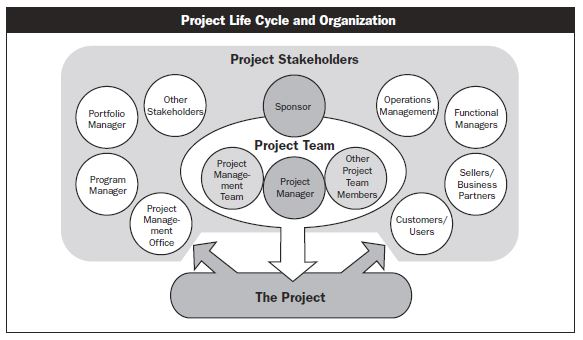
\includegraphics[width=\linewidth]{Bilder/Stakeholder_Uebersicht.jpg}
	\caption{Überblick Stakeholder. Alle am Projekt beteiligten Personen oder Organisationen müssen beachtet werden. Grafik entnommen aus \autocite[S. 24]{PMBOK}.}
	\label{StakeholderÜbersicht}
\end{figure}

Wihlidal beschreibt ein weit verbreitetes Problem welches durch Fehler in der Stakeholder analyse entsteht:
\begin{quote}
It is very important to ask the right questions to your stakeholders [...] a lot of design and development time is wasted because of incorrect user requirements. Getting them right from the start will help alleviate this problem.
\autocite[S. 28]{Wihlidal2006}
\end{quote}

In der Praxis wäre für die Konzeption bzw. das Systemdesign eines neuen Tools der Besuch der von der Tool Entwicklung betroffenen Teammitglieder am Arbeitsplatz und das beobachten der jeweils verrichteten Aufgaben sehr aufschlussreich. Durch diese Methode könnten Probleme im Arbeitsablauf frühzeitig identifiziert, behoben und besonders wichtige Features rechtzeitig vor Beginn der Implementierung in Erfahrung gebracht und geplant werden.

\autocite{Wihlidal2006} beschreibt Stakeholder bezüglich des Gebietes Tool Development folgendermaßen:
\begin{quote}
“They (Stakeholders, Anmerkung des Autors) are the users who are most affected by the introduction of a tool and they ultimately contribute to the design and goals. Stakeholders are (Anmerkung des Autors) defined as anyone who stands to gain or lose from the succes or failure of an application [...].” \autocite[S. 4-5]{Wihlidal2006}
\end{quote}
Diese Definition deckt sich mit der bereits erwähnten allgemeinen Definition der Stakeholder. Sollte für das Softwareprodukt keine Veröffentlichung der Tools zur Generierung von User Generated Content geplant sein, beschränkt sich der Kreis der Stakeholder auf das interne Entwicklerteam. Eventuell sind noch andere Publishereigene Studios und Teams zu berücksichtigen. Dies kann vor allem dann der Fall sein, wenn eine Spiele Engine in mehreren Studios eines Publishers eingesetzt wird. Als Beispiel sei hier die 3D Engine Frostbite Engine \footnote{\fullcite{FrostbiteEngine}} von Digital Illusions CE \footnote{\url{http://www.frostbite.com}} unter dem Publisher Electronic Arts \footnote{\url{http://www.ea.com}} angeführt. Dieser Publisher setzt für alle aktuellen Projekte\footnote{\url{http://www.frostbite.com/games/future-games/}} seiner Studios auf die gleichen Tools und die gleiche Engine.

Aus diesen Gründen ist eine Stakeholderanalyse (auch bei kleineren Projekten) ein Wichtiger Bestandteil des Entwicklungsprozesses. Eine Bedarfsanalye und eine allgemeine Analyse der Aufgabengebiete der jeweiligen Entwickler sollte in das System Design bzw. das Requirements Engineering ebenfalls mit einfließen. Hierzu könnten Interviews (Gespräche und Befragungen zu den Wünschen der Anwender) mit den Anwendern geführt werden. Dies ist eine schnelle Methode welche sich gut mit einem agilen Prozess wie Scrum oder iterativen Prozessen vereinbaren lässt.

\subsection{Prozess der Stakeholderanalyse}
Die Stakeholderanalyse wurde in folgenden Schritten durchgeführt und skizziert. Da diese Arbeit sich nicht auf ein reales Team bezieht, wurden statt der jeweiligen Personen oder Organisationen die Berufsbilder der eigentlichen Personen in den Vordergrund gestellt.
\begin{itemize}
\item Identifizieren der Stakeholder durch kreative Techniken wie z.B. Brainstorming
\item Stakeholder in eine Gittergrafik einteilen um ihre Nähe zum Projekt zu bestimmen
\item Interpretation der Stakeholder Absichten während des Projekts
\item Entwickeln von Maßnahmen um:
	\begin{itemize}
	\item Risiken zu identifizieren
	\item Beteiligungen im Projekt herauszuarbeiten
	\item Eine Umsetzungsstrategie zu entwickeln
	\end{itemize}
\end{itemize}

Der dritte Punkt die Interpretation der Absichten und Einstellung des jeweiligen Stakeholder zum Projekt entfällt in diesem Fall. Es ist ohne konkrete Personen schlicht nicht möglich eine persönliche fachliche Meinung des Stakeholders zu repräsentieren. Es wird an Stelle dessen hier davon ausgegangen, dass jeder Stakeholder ein Benutzerfreundliches praktisches Tool erhalten möchte welches den definierten Anforderungen dieser Arbeit entspricht.

\subsubsection{Identifizieren der Stakeholder}
Die Stakeholder wurden durch die kreative Methode eines Brainstormings als folgende Berufsgruppen innerhalb des Entwicklerteams des Unternehmens identifiziert. Auf Personengruppen außerhalb des Entwicklerteams wie z.B. Finanzabteilungen etc. soll nicht eingegangen werden, da sich diese Arbeit mit dem Prozess zur Konzeption eines Tools und der eigentlichen Konzeption zu diesem beschäftigt.
\begin{itemize}
\item Engineer
	\begin{itemize}
	\item Tool Eng.
	\item Graphic Eng.
	\item Network Eng.
	\item Articicial Intelligence Eng.
	\end{itemize}
\item Artist
	\begin{itemize}
	\item Animator
	\item World Builder / Level Designer
	\end{itemize}
\item Game-Designer
	\begin{itemize}
	\item Level Designer
	\item Game Logic Scripter
	\item User Interface Designer
	\end{itemize}
\item Producer
	\begin{itemize}
	\item Development Producer
	\item Publisher Producer
	\end{itemize}
\end{itemize}
Die Producer werden innerhalb der Konzeption dieser Arbeit als Designer betrachtet und unter dieser Gruppe geführt. Sollten die Producer denn Aufgaben an der Entwicklung übernehmen sind diese meist deckungsgleich mit den Aufgabenstellungen der Designer. Trotz allem sind die Producer hier aufgrund ihrer tragenden Rolle im Projekt als Stakeholder identifiziert worden. In vielen Fällen haben sie auch massive Entscheidungsgewalt über die verwendeten Techniken und Ressourcen während des Projektverlaufs.

\subsubsection{Involvement in das Projekt erkennen und bestimmen}
Um zu erkennen in welchem Bezug ein Stakeholder zu einem Projekt steht, wurde ein Gittermodell \ref{StakeholderGrafik} der Entwickler erstellt. Hier finden sich Beispielhaft weitere Stakeholder zur Verdeutlichung der Grafik. Hierzu zählen der Publisher, welcher als Organisation auftritt und weitere Entwicklerteams des gleichen Publishers die möglicherweise mit der gleichen Engine und evtl. den gleichen Werkzeugen arbeiten.
\begin{figure}[ht]
	\centering
	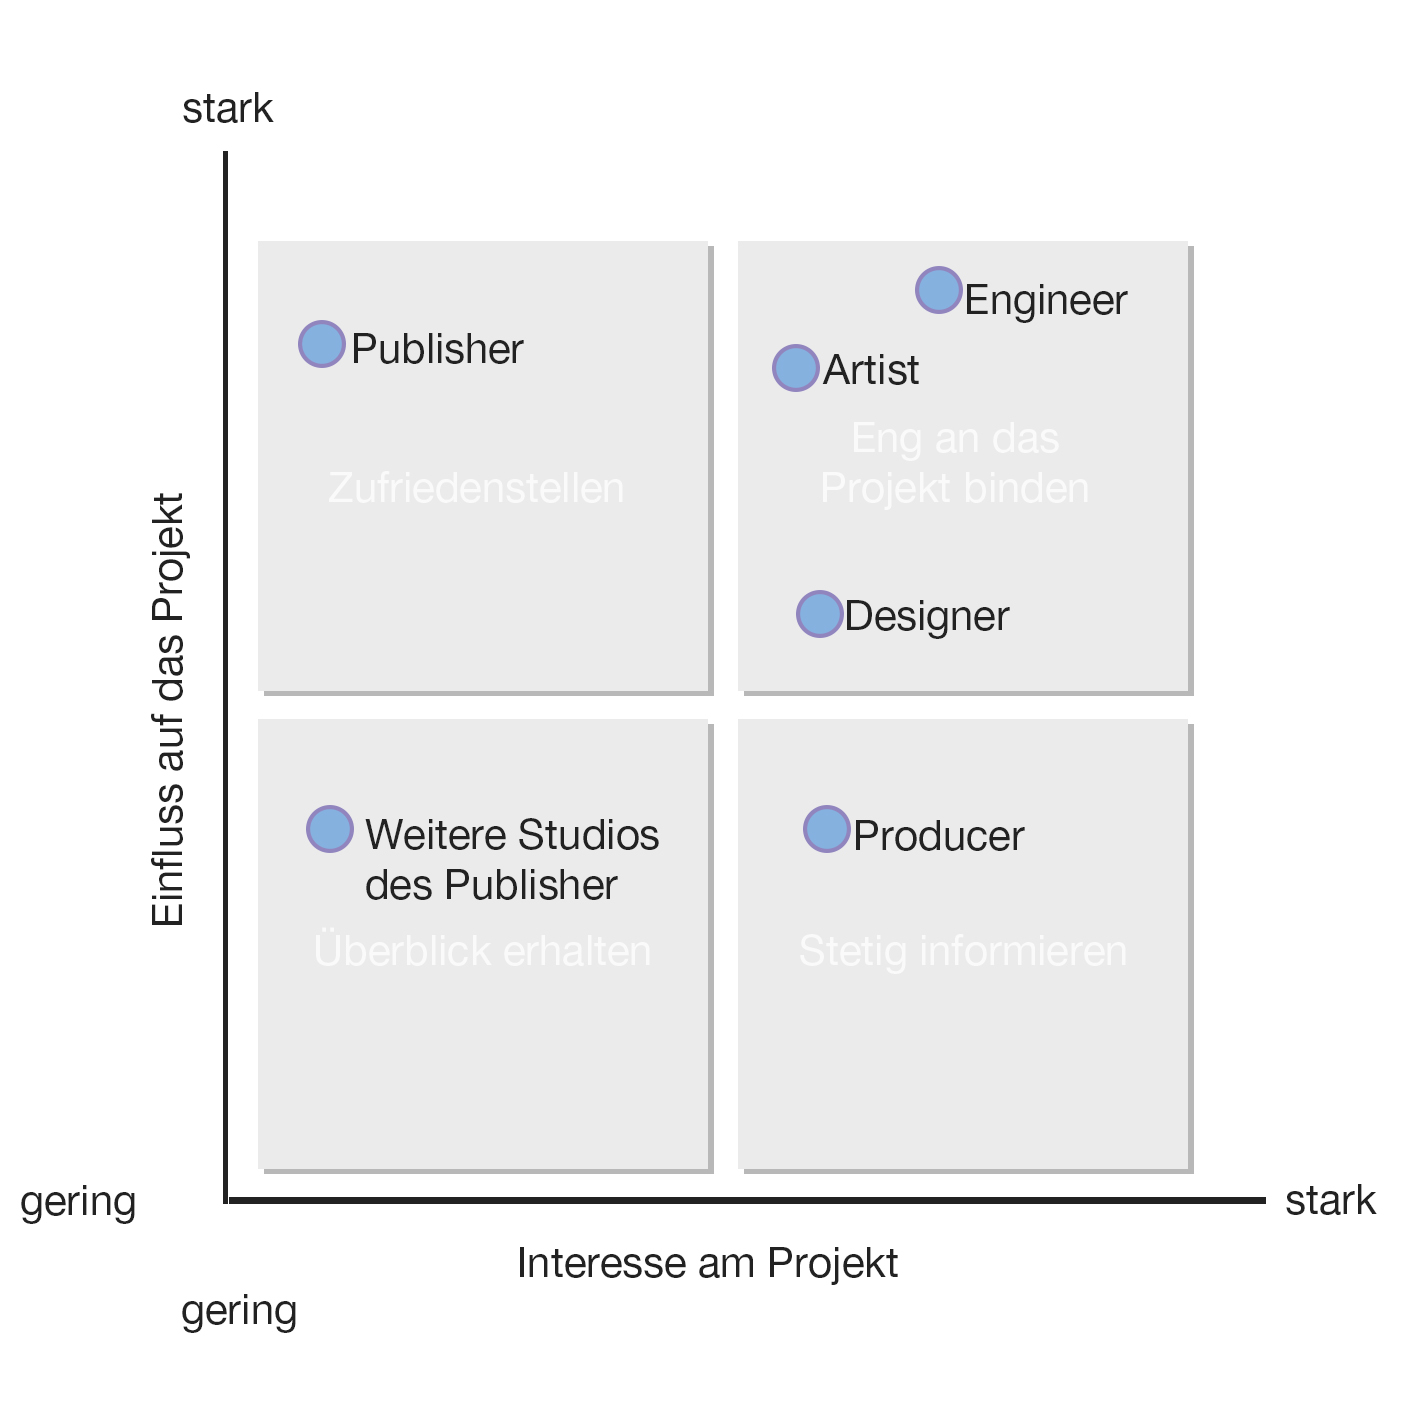
\includegraphics[width=\linewidth - 2cm]{Bilder/Stakeholder_Diagramm.jpg}
	\caption{Überblick über die Identifizierten Stakeholder und deren Inovelement in die Planung und Umsetzung des Tool Projektes.}
	\label{StakeholderGrafik}
\end{figure}
Mithilfe der ermittelten Stakeholder und den oben angeführten Projektmanagementmodellen kann nach dieser Analyse ein Prozess und ein Konzept für ein Tool entwickelt werden. Die nächsten Abschnitte beschäftigen sich mit der Entwicklung eines Arbeitsprozesses zur Konzeption eines Software Tools und dessen Umsetzung auf Basis der jetzt durchgeführten Analysen.

\section{Zusammenfassung des Arbeitsprozesses}
Zu Beginn des Tool Development Projektes sollte erst einmal die Struktur des Entwickler Teams analysiert werden. Hierbei muss sich für eine der möglichen Methoden der Organisation entschieden werden. Die beiden von Wihlidal \cite[S. ]{Wihlidal2006} beschrieben Organisationsstrukturen "Dedicated Tools Team" und "Content Team Develops and Supports" wurden als praktisch für das interne zur Produktentwicklung parallel ausgerichtete Tool Development vorgestellt. Sobald sich das Entwickler Team für eine Struktur entschieden hat, kann es sich um die Auswahl eines geeigneten Projektmanagementmodells kümmern. Hierbei wurde aufgrund seiner unkomplizierten Art und einfachen adaption das Scrum Projektmanagementmodell ausgewählt. Es vereinfacht den Entwicklungsprozess und reduziert den nötigen Verwaltungsaufwand auf ein Minimum.
Nach der Planung der Organisationsstrukturen kann das Team soch dem Konzeptionellen Part widmen und diesen mit einer Requirements Analyse beginnen. Diese Phase der Entwicklung ist mit größt möglicher Sorgfalt auszuführen da alle weiteren Schritte, insbesondere der Erfolg der Implementierung hiervon abhängig sind. In dieser Phase war es nötig, die Stakeholder zu identifizieren, UseCases zu verstehen und die benötigten Features der Software herauszuarbeiten. Im Anschluss an die Analyse folgt das Requirements Engineering. Hierbei handelt es sich um einen Arbeitsschritt welcher technische und theoretische Praktiken vereint. Eventuell werden während der Requirements Analyse auch besonders kritische Features durch eine Prototypische Implementierung ergründet. Weiterhin entsteht hier das gesamte Systemdesign.
Die Implementierungs und Testphase schließt das Projekt ab. Hierbei wird der Erfolg aller vorherigen Phasen auf die Probe gestellt. Die Implementierung kann von Alpha und Beta Tests begleitet werden. Somit können die Mitglieder des Produktionsteams das Tool bereits kennen lernen und einige Features in Rücksprache mit den Entwicklern noch verändern.
Der hier skizzierte Prozess wurde so weit es möglich war auch auf die Konzeption des FuseeAT angewendet.

\chapter{Entwicklung eines Konzeptes}

\section{Zeitersparnis durch die Entwicklung eines Tools als Plugin für eine bekannte Umgebung}
%TODO: Hier darauf eingehen warum in C4d und wieso und warum das den flow unterstützen könnte.
Im Gegensatz zu großen Monumentalen Editoren wie denen in der Unreal Engine 4 und der Unity Engine sieht das hier angewendete Konzept des Tool splitting vor, die verschiedenen Entwickler Disziplinen auf bekannte Tools aufzuteilen und diese bereits bekannten Tools mit neuer Funktionalität auszustatten. So minimiert sich die Einarbeitungszeit der Entwickler. Weiterhin sollte die Konzentration der Entwickler auf einem höheren Level erhalten bleiben als es bei Entwicklern der Fall ist, welche für jeden Schritt das Tool wechseln müssten. Natürlich bieten bereits jetzt große Editoren wie Unreal Engine 4 und Unity fast jegliche Funktionaltität in einem großen Tool an, wie aber bereits gesagt ist es nötig dazu die bereits erlernte Software wie z.B. Cinema 4D zu verlassen.

Eine Zeitersparnis auf Seiten der Tool Entwickler kann erreicht werden, da sie sich nur mit der Erweiterung einer bereits fertiggestellten, getesteten Software beschäftigen müssen anstatt ein komplett neues Tool zu entwickeln. Es entfällt hierbei ein großer Teil der Software Architektur. Natürlich gibt es auch hier einschränkungen. Das zu erweiternde Tool muss den Tool Developern bekannt und eine Schnittstelle vorhanden sein. Im Rahmen dieser Arbeit konnten beide Bedingungen ausreichend erfüllt werden. Cinema 4D bietet eine Schnittstelle in Form einer API und das Tool war dem Autor aus früheren Projekten ausreichend bekannt.

Das hier entwickelte Konzept versucht nun die in der Analyse gewonnenen Erkenntnisse über den Entwicklungsprozess umzusetzen und dabei ein Tool zu konzipieren welches den Cinema 4D Model Editor um Fusee Editing Funktionalität erweitert. Hierbei wird die Pluginfunktionalität von Cinema 4D als Schnittstelle zum Benutzer ausgenutzt. Das konzipierte Plugin nutzt im Hintergrund als Businesslogik das FuseeAT und beinhaltet selbst nur Funktionalität welche durch die Cinema 4D API bedingt wird. Begonnen werden aber soll die Konzeption des Tools mit einer Analyse des Teams und dem Erstellen von Use Cases.

% Planung
\section{Use Cases der verschiedenen Entwickler}
Diese Abschnitt behandelt eine Auswahl alltäglicher Tasks (z. Dt. Aufgaben) der Mitarbeiter des Produktionsteams und die Arbeitsschritten die dazu nötig sind diese zu erledigen. Aus den aufgelisteten Tasks wurden dann die Anforderungen für die Requirementsanalyse herausgearbeitet. Um an diese Auflistung heranzukommen, empfiehlt sich in der Praxis das Interviewen und das Beobachten von Teammitgliedern um den Arbeitsalltag und die Probleme die das Tool lösen soll besser zu verstehen. Weiterhin können Ziele des Projektes und spezielle kritische Marken im Gamedesign Aufschluss über benötigte Features liefern.

\subsection{Use Cases für Artists}
Es folgt eine Auflistung der Tasks die den normalen Arbeitsablauf eines Artists in der der Entwicklung mit der Fusee Engine bezeichnen. Um die Tasks zu ermitteln wurde sich verschiedener kreativer Hilfsmittel wie z.B. Mindmaps und Brainstorming bedient. Die folgenden Use Cases beschreiben die Tätigkeiten von Artists im Fusee Authoring Tool.
\begin{itemize}
\item Asset erstellen
\item Asset exportieren
\item Szene erstellen
\item Szene bearbeiten
\item Szene speichern
\end{itemize}

Die Übersicht \ref{UseCaseArtist} beschreibt die Einbindung des Artist in das System und skizziert seine Use Cases in Verbindung mit den Modulen des gesamten Systems. Das Modul “Project Handler System” beschreibt hier eine imaginäre Editoren Schnittstelle zwischen den anderen Modulen.
\begin{figure}[ht]
	\centering
	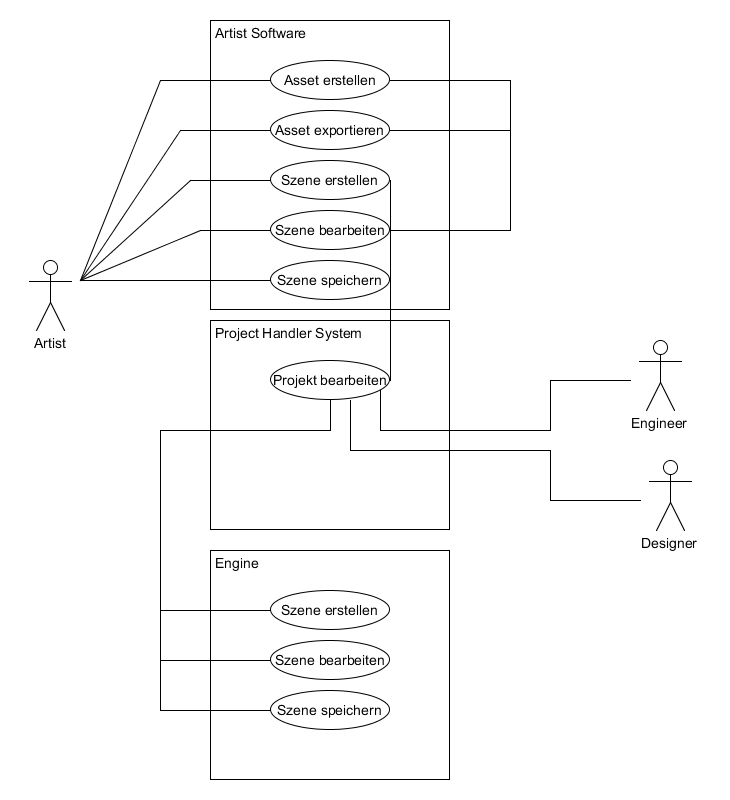
\includegraphics[width=\linewidth]{Bilder/UseCase_Artist.png}
	\caption{Überblick über die Use Cases eines Artist.}
	\label{UseCaseArtist}
\end{figure}

Es folgt eine Betrachtung der einzelnen Tasks vom Standpunkt des Requirementsengineering aus. Anschliessend wurden die wichtigsten Aktivitäten eines Tasks herausgefiltet und hierraus ein System entwickelt.

\subsubsection{Asset erstellen}
Der Artist erstellt ein Asset in seiner gewohnten Software. Normalerweise handelt es sich hier um 3D Modelle oder 2D Texturen. Texturen werden in einem 2D Grafikprogramm erstellt und  in das 3D Programm importiert. Es folgt das mapping auf die Modelle.

\subsubsection{Asset exportieren}
Ein Modell wird vom Artist exportiert und in der Projekstruktur gespeichert. Dieses verorten in der Projektstrutkur übernimmt das Plugin. Das Asset wird in die Solution Dateien integriert.

\subsubsection{Szene erstellen}
Eine Szene wird über das Interface der 3D Applikation erstellt und in der Projektstruktur über das Plugin verortet.

\subsubsection{Szene bearbeiten}
Eine bereits bestehende Game Szene kann vom Artist bearbeitet werden.

\subsubsection{Szene speichern}
Eine Szene wird vom Artist gespeichert und steht danach anderen zur Bearbeitung zur Verfügung.

\subsection{Use Cases für Designer}
Die Use Cases von Designern bilden sich häufig aus einer Schnittmenge der Use Cases von Artists und Engineers. Was Designer einzigartig macht ist meist ihr Überblick über die gesamte Entwicklung. Folgende Usse Cases beschreiben die Tasks von Designern im geplanten Fusee Authoring Tool. Das Use Case Diagramm \ref{UseCaseDesigner} visualisiert die aufgeführten Use Cases.

\begin{figure}[ht]
	\centering
	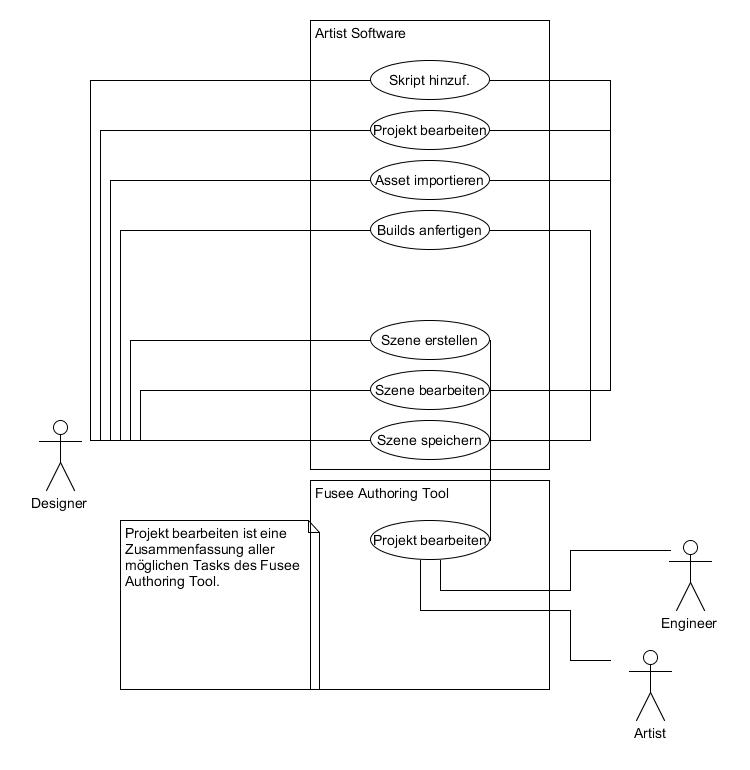
\includegraphics[width=\linewidth - 2cm]{Bilder/UseCase_Designer.jpg}
	\caption{Überblick über die Use Cases eines Designers.}
	\label{UseCaseDesigner}
\end{figure}

\begin{itemize}
\item Skript-Datei hinzufügen
\item Asset importieren
\item Projekt bearbeiten
\item Builds anfertigen
\item Szene erstellen
\item Szene bearbeiten
\item Szene speichern
\end{itemize}

\subsubsection{Skript-Datei hinzufügen}
Eine Skript Datei wird an ein Objekgt angefügt. Im Falle von Fusee handelt es sich hier entweder um Javascript Code für Web Builds oder um eine \CSS Code Datei.
\subsubsection{Asset importieren}
Der Designer kann vom Artist erstelle Assets in eine Szene des Editors importieren. 
\subsubsection{Projekt bearbeiten}
Der Designer bearbeitet das Projekt. Dies bedeutet er muss das Projekt öffnen und betrachten können.
\subsubsection{Assets platzieren, skalieren und transformieren}
Der Designer platziert verschiedenste Assets in die erstellten Welten mit Hilfe des Editors. Er skaliert diese Assets auf die korrekte Größe und transformiert ihre Position im Raum. Somit passt er die vom Artists erhaltenen Assets an seine eigenen Bedürfnisse an. 
\subsubsection{Builds anfertigen}
Das erstelle Spiel wird durch einen Build getestet. Sollte ein Build erfolgreich sein, kann der Designer seine erstellen Welten und Level in der Fusee Applikation ausprobieren. Er kann die Wirkung der Welt beurteilen und möglicherweise Veränderungen am Design und Layout vornehmen.
\subsubsection{Szene erstellen, Szene bearbeiten, Szene speichern}
Diese drei UseCases sind deckungsgleich mit denen des Artist und werden aus diesem Grund hier nicht mehr gesondert beschrieben.

\subsection{Use-Cases eines Engineer}
Engineers bewegen sich eher auf der technischen Seite der Entwicklung und beschäftigen sich demnach im Fall von Fusee hauütsächlich mit einer IDE wie Visual Studio. Die hier aufgeführten Tasks beschreiben die Use Cases eines Engineers im Bereich des Fusee Developments.

\begin{itemize}
\item Code-Datei hinzufügen
\item Asset verwenden
\item Projekt bearbeiten
\item Builds anfertigen
\item Szene erstellen
\item Szene bearbeiten
\item Szene speichern
\end{itemize}

Die Übersicht \ref{UseCaseEngineer} skizziert die Verwebung des Engineer mit seinen Use Cases und dem System.
\begin{figure}[ht]
	\centering
	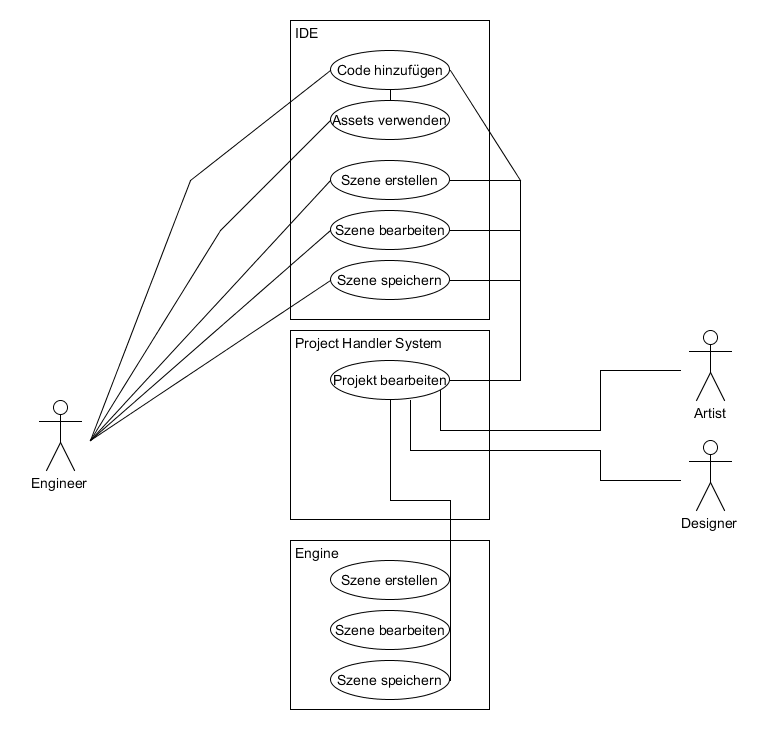
\includegraphics[width=\linewidth]{Bilder/UseCase_Engineer.png}
	\caption{Überblick über die Use Cases eines Engineer.}
	\label{UseCaseEngineer}
\end{figure}

Der Engineer beschäftigt sich mit einem programmierlastigeren Aspekt des Projektes. Zu seinen Aufgaben gehört die Verwaltung des Projekts und das Verwenden der vom Artist erstellten Assets.

\subsubsection{Code-Datei hinzufügen}
Der Engineer möchte neu geschriebenen Code in das Projekt einfügen. Ersucht sich somit die passende Stelle und kann den Code in der Projektstruktur erzeugen / einfügen. Der Code wird durch die IDE in der Projektstruktur untergebracht.

\subsubsection{Asset verwenden}
Der Engineer verwendet Assets (Models, Texturen, etc.) um diese in einer Szene anzuprogrammieren. Hierzu wird das Asset durch Code in die Engine geladen, texturiert und mit Shadern versehn etc. Bei einem Build wird das Model korrekt kopiert bzw. in das Build Format überführt.

\subsubsection{Projekt bearbeiten}
Der Engineer verändert etwas an der Projektstruktur oder der Codebase des Projektes. Die Änderungen werden dauerhaft gespeichert und in der Projektstruktur verortet.

\subsubsection{Szene erstellen}
Der Engineer erstellt während des hinzufügens von Code eine neue Szene in der GameEngine. Diese neue Szene hat verschiedene im Code übergebene Eigenschaften. Der ProjectHandler muss diese Szene möglicherweise registrieren und so für eventuelle Artists in der jeweiligen Software zugänglich machen.

\subsubsection{Szene bearbeiten}
Der Engineer öffnet eine Szene und bearbeitet diese in seiner IDE. Hierzu muss der ProjectHandler die Szene bereitstellen und mögliche Änderungen verwalten und an Artists weitergeben.

\subsubsection{Szene speichern}
Eine Szene wird gespeichert und vom ProjectHandler in ein Format überführt welches ein Artist in seiner gewohnten 3D Umgebung ebenfalls nutzen kann.

\section{Ananlyse von beliebten Editoren und derer Module im Bezug auf die Konzeption des FuseeAT Plugins}
Aufgrund der Thematik mit dem Bezug zur 3D Engine Fusee beschränkt sich die Auswahl der betrachteten Editoren auf die an der Hochschule Furtwangen populärsten Game Engines und Editoren, analysiert deren Editoren Features und stellt die Arbeitsabläufe in diesen Editoren und Tools dar. Es folgt eine Wertung und ein Vergleich mit den für das Fusee Authoring Toolkit geplanten Features. Bei den hier gewählten Editoren handelt es sich um stand alone Applikationen welche das Gegenteil des hier entworfenen Konzeptes eines in das Content Creation Tool integrierten Editors darstellen. Allerdings gleichen sich die Authoring Tool Ansätze maßgeblich. Funktionen, Module und Konzepte sind größtenteils deckungsgleich mit denen des Cinema 4D Editors. Aus diesem Grund lassen sich einige der Module für FuseeAT und vor allem das Cinema 4D Plugin adaptieren.

\subsection{Unreal Engine 4}
Die UnrealEngine4\footnote{\fullcite{UnrealEngine4}} (kurz UE4) wird von EPIC Games Inc. entwickelt und stellt eine im grafischen Sektor im High End Bereich angesiedelte Game Engine dar. Bei ihr handelt es sich um eine an einen Authoringeditor (Welt Editor / Level Editor) gebundene Game Engine.Alle Teile des Projekts kommen in diesem Editor zusammen und Projekte müssen dort bearbeitet werden. Die Engine sieht die Verwendung von Visual Studio 2013 auf Windows Rechnern und der IDE XCode auf Mac Rechnern zum schreiben von Code und dem kompilieren von Projekten vor. Seit kurzem ist die Unreal Engine kostenfrei unter \url{http://www.unrealengine.com} zu beziehen. Sollte ein mit der UE4 entwickeltes Produkt kommerziell vertrieben werden, so sind 5\% des Umsatzes an Lizenzgebühren an EPIC zu bezahlen.

Sourcecode wird in der Unreal Engine in C++ und Blueprint geschrieben. Bei Blueprint handelt es sich um eine von EPIC entwickelte Visual Scripting Language (ein Node basiertes System) die sich verstärkt an Designer und Artists richtet.

Die UE4 kann Builds für folgende Plattformen erzeugen:
\begin{itemize}
\item Windows PC
\item Linux
\item Mac
\item iOS
\item Android
\item XBox One (In Verbindung mit einer DevKit Lizenz zu erwerben bei Microsoft.)
\item Playstation 4 (inkl. dem noch nicht veröffentlichten VR Projekt Morpheus) (In Verbindung mit einer DevKit Lizenz zu erwerben bei Sony.)
\end{itemize}

Plattformen auf welchen mit der Unreal Engine entwickelt werden kann sind:
\begin{itemize}
\item Windows PC
\item Mac OSX
\item Linux (in Entwicklung, unstable)
\end{itemize}

Der Sourcecode der Unreal Engine steht auf GitHub\footnote{\url{https://www.unrealengine.com/ue4-on-github}} zur freien Verfügung. Aus diesen Gründen wird die aktuellste Version der Unreal Engine, Version 4, für die Analyse dieser Arbeit zugrunde gelegt.

Der Unreal Engine 4 Editor ist sehr flexibel an die eigenen Bedürfnisse anpassbar. Abhängig von den Wünschen der Entwickler kann die Oberfläche mehr auf das Entwickeln oder Designen ausgerichtet werden und bietet ähnliche Funktionen wie z.B. das Modeling Programm Cinema 4D. Der Editor bietet zu fast jeder Aktion eine Grafische Oberläche an. So genannte Projekt Wizards, führen den Benutzer bei komplexeren Prozessen an der Hand und erleichtern ihm so die Konfiguration von Assets im Editor. Sie unterstützen z.B. beim erstellen einer neuen Klasse oder dem Anlegen eines neuen Materials. Diese Wizards sind besonders für Neueinsteiger nützlich. Sie verdeutlichen den Ablauf eines Prozesses und unterstützen ein Fehlerfreies Abarbeiten der unterstützen Aktion.

\subsubsection{Coding in der Unreal Engine 4}
Anwendungen in der UE4 können mit Hilfe von verschiedenen Codingmechanismen erstellt werden. Die erste Möglichkeit wäre die dauerhafte Verwendung des Editors und des Konzeptes des Visual Programming mit Hilfe des Unreal eigenen Blueprint Systems. Beim Visual Programming handelt es sich wie die Bezeichnung bereits andeutet um visuelles Programmierung mit Hilfe von Grafischer Darstellung des Codes anstelle der Darstellung als Text. Hierbei werden oft Systeme eingesetzt die auf Nodes basieren. Die Abbildung \ref{UE4Blueprint} zeigt einen Ausschnitt aus einem Visual Programming Code welcher mit Blueprint erstellt wurde. Als Blueprint wird eine zusammengesetze Konfiguration aus Assets und Node basiertem Code bezeichnet.

\begin{figure}[ht]
	\centering
	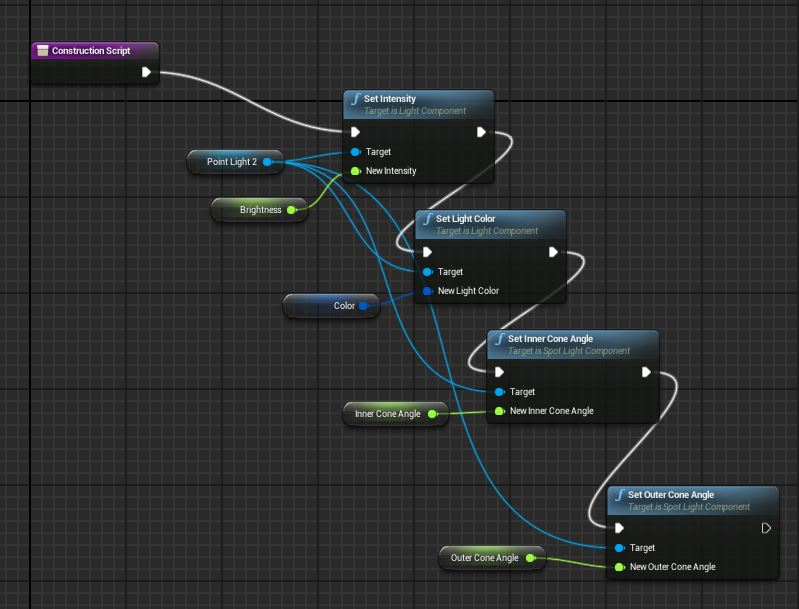
\includegraphics[width=\linewidth]{Bilder/ue4Blueprint.jpg}
	\caption{Programmierung in der Unreal Engine 4 mit Hilfe des Blueprint Visual Programming Systems/Interfaces}
	\label{UE4Blueprint}	
\end{figure} 

Die etablierte Programmiersprache C++ ist zweite Möglichkeit mit der UE4 Code zu schreiben. Allerdings hat EPIC die Unreal Engine Compiler dahingehend erweitert, dass ein spezielles Reflection System für die UE4 spezielle Sprachkonstrukte erkennen und in der Engine verwenden kann. Das Beispiel \ref{UE4_Makros}\footnote{Entnommen und abgeändert/erweitert aus der C++ Datei UECodeAnalysisProjectile.h des Beispiels “First Person Scene” des Unreal Engine 4 Editors.} zeigt mehrere solcher Markup Befehle vor den jeweiligen Funktionen, Properties der Klasse. Es handelt sich hierbei um Bezeichnungen wie z.B. UENUM(), UCLASS(), USTRUCT(), UFUNCTION(), und UPROPERTY().

\lstinputlisting[language=C++, caption = Unreal Engine C++ Header Datei. Makros als Markup Befehle, label=UE4_Makros]{Code/ue4makros.h}

Diese Makros und weitere sind alle in der UE4 Dokumentation \url{https://docs.unrealengine.com/latest/INT/} aufgelistet. Allerdings ist diese Art der Deklaration nur für bestimmte Schnittstellen Klassen essentiell. Der meiste selbst geschriebene Code kann ohne diese Makros geschrieben werden. Sie dienen nur der Kommunikation mit dem Editor und Kernsystemen der Engine. Es ist aber zu empfehlen diese Möglichkeit zu nutzen, so kümmert sich Beispielsweise der Garbage Collector der UE4 um Properties und Objekte welche mit den korrekten Makros ausgezeichnet wurden. 
\begin{quote}
For instance, a variable with a declaration prefaced by a UPROPERTY() macro can be garbage collected by the engine, and can be displayed and edited within Unreal Editor. \autocite{UnrealEngine4} - Dokumentation Unreal Engine 4 \url{https://docs.unrealengine.com}.
\end{quote}
Der gesamte C++ Code eines Projektes wird je nach Entwicklungsplattform entweder in Visual Studio (auf Windows) oder in der IDE XCode (auf Mac OSX) geschrieben. In der Realität werden Projekte mit einer Mischung der beiden Möglichkeiten (C++ und Blueprint) umgesetzt. Für das schnelle Prototyping eignet sich aber Blueprint alleine bereits sehr gut.

\subsubsection{Asset Verwaltung in der Unreal Engine 4}
Assets können in der Unreal Engine 4  z.B. im Dateiformat .fbx (Version 2013) Importiert werden. Die Modelle und Materialien können hierbei z.B. direkt in 3DS Max, Modo oder Cinema 4D erstellt und übernommen werden. Es ist also möglich, die UE4 direkt in die AssetPipeline einzubinden. Durch die offene Verfügbarkeit des Quellcodes können auch eigene Module für die UE4 geschrieben werden, welche die Assetpipleine erweitern. Die Unreal Engine bietet einen Contentbrowser (siehe Abbildung \ref{UEContentbrowser}) an, welcher es ermöglicht Assets zu sortieren und diese zu durchsuchen. Assets können dann per Drag and Drop in die Szene der Engine eingefügt werden. Eine solche Lösung ist optimal um Designer und Artists bei ihrer Arbeit zu unterstützen.

\begin{figure}[ht]
	\centering
	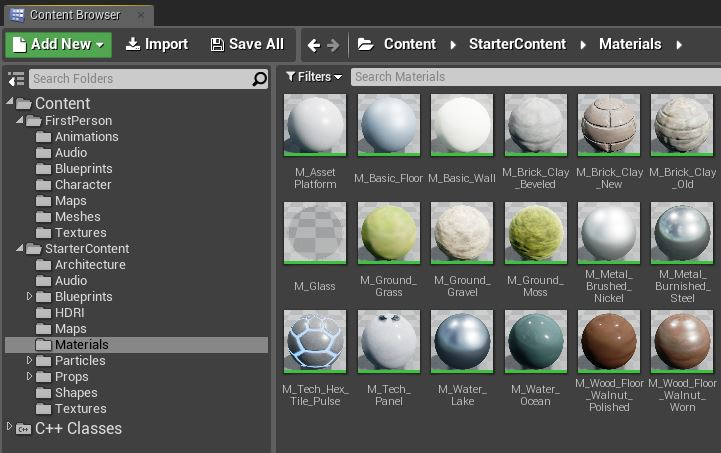
\includegraphics[width=\linewidth]{Bilder/UE_Contentbrowser.JPG}
	\caption{Ansicht des Contentbrowsers der Unreal Engine 4. Mit Suchfeld und Filterfunktionen, Assetvorschau ausklappbarer Ordnerstruktur.}
	\label{UEContentbrowser}
\end{figure}

Zur Versionsverwaltung von Assets ist die Möglichkeit zur Integration eines Versionskontrollsystems gegeben. Eingebunden werden können auf GIT, Subversion und Perforce basierte Systeme.

\subsubsection{Szenengraph in der Unreal Engine}
Hier gehts um den UE4 Szenengraphen \ref{UESzenenGraph} und seine Gemeinsamkeiten mit dem Fusee und Cinema 4D Szenengraphen.
\begin{figure}[ht]
	\centering
	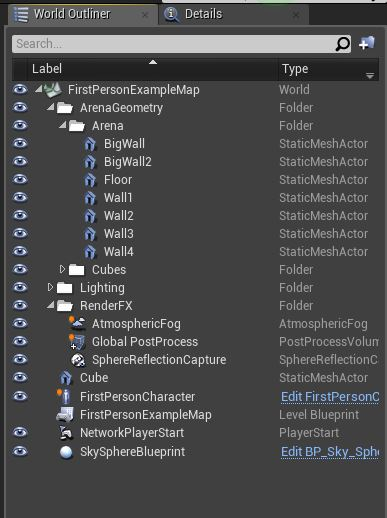
\includegraphics[width=9cm, height=10cm]{Bilder/UESzenenGraph.JPG}
	\caption{Beispielhafte Szene im Szenengraph der Unreal Engine 4. Er gleicht dem Fusee und Cinema 4D Szenengraphen stark.}
	\label{UESzenenGraph}
\end{figure}
Der Szenengraph hängt unmittelbar mit der Detailansicht der Elemente zusammen. In der Detailansicht können jegliche “Components” an einem Objekt der Szene betrachtet und verändert werden.

\subsubsection{Was kann für das FuseeAT Konzept aus der UE4 übernommen werden?}
Um mit der Unreal Engine effektiv zu arbeiten, muss jeder Entwickler das Tool von Grund auf neu erlernen. Genau diese Problematik soll FuseeAT umgehen indem es bereits bekannte Tools, für diese Arbeit Cinema 4D, verwendet um eine von den Mitarbeitern bereits erlernte Oberfläche weiter zu verwenden. Allerdings bietet auch eine so komplexe und tief gängige Engine wie die Unreal Engine 4 Ansätze die für das Fusee AT interessant sind. Das Blueprint System funktioniert wirklich gut und unterstützt Game Designer und Skripter während ihrer Arbeit und bietet ihnen eine gut durchdachte Visual Programming Lösung für die täglichen Aufgaben an. Ein solches System könnte sich in FuseeAT in Zukunft ebenfalls umsetzen lassen. Diese Funktionalitäten wurden bereits an der Hochschule Furtwangen in einem Projekt (Circuit 3D 2011 bis 2012) bei Herrn Prof. Müller diskutiert und an implementiert. Ein Teil der Ergebnisse dieses Projektes fand damals den Weg in das Fusee Projekt Uniplug.
Weiterhin sind die Makros bzw. das Markup System ein guter Ansatz, Code zu markieren um im FuseeAT darauf einzugehen. \CSS bietet hier mit seinem Reflection und Attributes System genügend Möglichkeiten diese Funktionalität in FuseeAT zu integrieren. Die Funktionen des Contentbrowsers der UE4 könnten in Cinema 4D über verschiedene API Funktionen nachgebildet werden. Der Szenengraph der UE4 gleicht dem Fusee und Unity 3D Szenengraphen stark. Es handelt sich bei dieser Ausgestaltung um eine Konvention im Sektor der 3D Engines und darum kann das System von Cinema 4D übernommen werden ohne voraussichtlich dem Arbeitsfluss der Designer und Artists zu schaden.

%--
%Sehr Komplex
%Viel neues zu lernen. Wahnsinnig Tiefgehend.
%Blueprints sind ein praktisches System aber man muss einen gewissen Wissensstand haben um zu finden was gesucht wird etc.
%Als Entwickler muss man mit dem Editor und dem Code in VS arbeiten.
%Blueprint ist sehr präsent und nicht mehr “nur” eine Skriptsprache wie das Kismet System in der UE3 sondern ein gesamtes System. Es wird als Zentrale Konfigurationsmöglichkeit angeboten. Man kommt eigentlich nicht daran vorbei. Prefabs möglichkeiten etc. Dazu konfigurationen und speichern etc. Instanzen können jedesmal anders eingestellt werden.

% Hier wichtig. Dazu schreiben wie ist er aufgebaut und welche Möglichkeiten hat man dort. Was bringt die Übersicht?


\subsection{Unity 3D}
Die Unity 3D Engine \footnote{\fullcite{UnityEngine5}} in der Version 5 wird von Unity Technologies entwickelt. Das Lizenzmodell sieht eine kostenfreie Variante mit einigen Einschränkungen und eine an Professionelle Nutzer gerichtete kostenpflichtige Version für in etwa 75\$ pro Monat vor. Enterprise Versionen, welche auch den Sourcecode der Engine enthalten, können über eine gesonderte Kontaktaufnahme gekauft werden. Die Unity Engine ist an den Unity Editor gebunden. In diesem Editor werden alle Entwickleraufgaben erledigt. Die IDE kann vom Programmierer frei gewählt werden. Es empfiehlt sich aktuell aber auf das von Unity mitgelieferte Mono Develop, Xamarin Studio oder Visual Studio in einer Version ab 2013 zu setzen. Vollen Support bietet aber aktuell nur das mitgelieferte Mono Develop. Unity unterstützt die Programmiersprachen \CS, Javascript und Boo. Bei Boo handelt es sich um eine von Unity Technologies selber entwickelte Skriptsprache.

Unity kann Builds für die folgenden Plattformen erzeugen:
\begin{itemize}
\item iOS
\item Android
\item Windows Phone 8
\item Black Berry 10
\item Windows
\item Windows Store
\item Mac OSX
\item Linux
\item Web Player
\item Playstation 3 *\footnote{* In Verbindung mit einer DevKit Lizenz zu erwerben bei Sony.}
\item Playstation 4 *
\item Playstation Vita *
\item Playstation Mobile *
\item XBox One **\footnote{** In Verbindung mit einer DevKit Lizenz zu erwerben bei Microsoft.}
\item XBox 360 **
\item Wii U  ***\footnote{*** In Verbindung mit einer DevKit Lizenz zu erwerben bei Nintendo.}
\end{itemize}

Als Entwicklerplattformen unterstützt Unity die Betriebssysteme Windows und Mac OSX. Der Sourcecode der Engine ist nur in einer Enterprise Version erhalten. Zum Erhalt dieser müssen gesonderte Verhandlungen mit Unity Technologies geführt werden. Aus diesen Gründen wird die kostenfreie “free” Version für die Analyse in dieser Arbeit zu Grunde gelegt.

\subsubsection{Coding in der Unity Engine 5}
In Unity 5 kann wie bereits erwähnt in \CS, Javascript und Boo entwickelt werden. Die beiden Skriptsprachen Javascript und Boo wurden für diese Arbeit nicht betrachtet, da sich auch Fusee für die Desktopentwicklung auf \CSS fokussiert hat. Unity bringt eine Version der Mono Develop IDE mit, welche alle drei Sprachen unterstützt. Unity unterstützt in der Version 5.0 aktuell das .Net Framework 3.5 und damit die \CSS Version 3.0 und die damit verbundenen Sprachfeatures. Unity setzt stark auf das Konzept des Programmierens mit Components. Die gesamte Engine ist für die Arbeit mit Components ausgelegt. Hierbei wird Funktionalität der Anwedungen so weit heruntergebrochen, bis sie in einzelne Code Dateien ausgelagert werden kann. Aus einem Pool an Component Skripts wird dann das Verhalten eines einzelnen Szenenobjekts aufgebaut. Dieses System ist sehr dynamisch und unterstützt die Entwickler beim experimentieren in der Game Engine. Eine solche Component basierte Lösung ist für das FuseeAT ebenfalls denkbar. Unity bietet genau wie die Unreal Engine einige Standardfunktionen welche im \CSS Code überschrieben werden sollten um ein Objekt in der Engine zu instanziieren. So wird ein GameObject (Die Bezeichnung eines Laufzeitobjektes in Unity) wie in Codebeispielt \ref{UnityGameObject} implementiert. Das Beispiel enthält keinen funktionalen Code sondern stellt lediglich die Struktur dar. Fusee wird keine dieser Strukturen einbinden. Das Arbeiten mit FuseeAT soll für den Programmierer so frei wie möglich gestaltet werden.

\lstinputlisting[caption = Unity GameObject Struktur, label=UnityGameObject]{Code/unityGameObject.cs}

FuseeAT wird auf eine solche Einschränkung der Programmierung verzichten. Das hat mehrere Gründe. Zum einen soll Fusee als Engine in der Lehre eingesetzt werden und hier besonders das Verständnis für tiefer gehende Prozesse einer Game Engine fördern. Zum anderen sollen jegliche Projekte mit der Fusee Engine durch einen einfachen Build auch im WebBrowser ausgeführt werden. Weiterhin ist die Fusee Engine ein großes Teamprojekt und deren Erweiterung in diesem Maße kann während dieser Arbeit nicht entschieden und/oder umgesetzt werden.

\subsubsection{Asset Verwaltung in der Unity Engine 5}
Die Verwaltung von Assets in Unity ist ein recht einfacher Prozess. Modelle und Grafiken werden in den jeweiligen Programmen wie z.B. 3DS Max, Cinema 4D, Photoshop oder anderer Grafik Software erstellt und im passenden Format einfach in den Projektordner von Unity kopiert. Das Asset kann dann im Unity Editor selbst noch auf das Projekt abgestimmt werden. Ein Modell kann Materialien erhalten, Texturen können getauscht und Grafiken skaliert und auf Objekte angewendet werden. Aus mehreren Assets und/oder Components können in Unity so genannte Prefabs erstellt werden. Bei diesen handelt es sich um ein Paket aus Assets und Code welches z.B. zur Laufzeit der Engine instanziiert werden kann. Prefabs könnten auch als Abbild eines GameObjects in einem spezifischen Moment (Der Moment ihrer Initialisierung) bezeichnet werden. Sie verhalten sich immer genau gleich wie das Ursprungs Prefab soweit sie nich individuell zur Laufzeit angepasst werden. Ein solches System ist für FuseeAT vorerst nicht geplant, könnte sich aber in der Zukunft als nützlich erweisen. Fusee kann bereits in Cinema 4D gemodelte Objekte oder Modelle in der Fusee Engine mit Hilfe von Prototype serialisieren, allerdings ist dieses System noch nicht zu Ende implementiert und wird stetig erweitert.

\begin{figure}[ht]
	\centering
	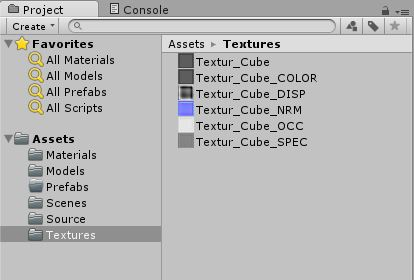
\includegraphics[width=7cm]{Bilder/uContentbrowser.jpg}
	\caption{Ansicht des Contentbrowsers in Unity. Mit Suchfeld und Filterfunktionen und ausklappbarer Ordnerstruktur.}
	\label{UnityContentbrowser}
\end{figure}
Um Assets in Unity zu bearbeiten, zu verwalten und zu durchsuchen steht ein Contentbrowser, siehe Abbildung \ref{UnityContentbrowser}, mit eben genau diesen Funktionen zur Verfügung. Grundsätzlich bildet dieser Contentbrowser alle Möglichkeiten ab, die auch FuseeAT unterstützen möchte.

\subsubsection{Szenengraph in Unity}
Der Unity Szenengraph gleicht dem Fusee Szenengraph. In der Tat lehnt sich das Design des Fusee Szenengraphen am System der Unity Engine an, denn beide basieren auf Nodes welche auf der gleichen Ebene durch Components erweitert werden. Kindobjekte von Nodes sind wiederum weitere Nodes. Dieses Design des Szenengraphen ist in Heutigen Game Engine bereits als eine Best Practice Lösung anzusehn und könnte aus diesem Grund auch Problemlos in FuseeAT integriert werden. Das System kann schnell durchdrungen und adaptiert werden.
\begin{figure}[ht]
	\centering
	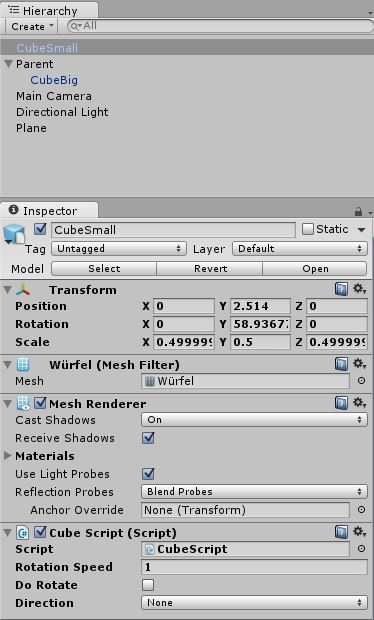
\includegraphics[width=7cm]{Bilder/uSzeneGraphDetails.jpg}
	\caption{Beispielhafte Szene im Szenengraph von Unity. Er gleicht dem Fusee und Cinema 4D Szenengraphen stark. Das Detailpanel zeigt Components eines Nodes.}
	\label{UnitySzenengraph}
\end{figure}

\subsubsection{Was kann für das FuseeAT Konzept aus Unity übernommen werden?}
Aus den Funktionen der Unity Engine können verschiedene interessante Konzepte gefunden und für FuseeAT adaptiert werden. Hierzu gehört zu aller erst das Component System. Die Unreal Engine setzt wie bereits erwähnt ebenfalls auf ein Component System und das neue Szenengraphen Modell in Fusee unterstützt diesen Ansatz ebenfalls. So sollte auch FuseeAT dieses Konzept berücksichtigen und die in Fusee möglichen Components auch in den Cinema 4D Editor integrieren. Weiterhin ist das einfache Build und Deploymentsystem von Unity eine stärke der Engine. Für FuseeAT wäre es ein guter Ansatz die Arbeit der Designer und Artists mit der Fusee Engine in Cinema 4D zu erleichtern wenn Builds für den Desktop und später evtl. auch Web-Builds eines gesamten Fusee Projekts (welche aktuell wie bereits erwähnt schon mit der Fusee Engine möglich sind) aus der C4D Software heraus erstellt werden könnten. Hiermit können  Designer und auch Artists jederzeit das Ergebnis ihrer Arbeit durch einen einfachen Build Vorgang direkt in der Engine betrachten.

%Einfachheit des Editors.
%Component System.
%Einfaches Materialsystem.
%Debugmöglichkeit ist gut, einfaches skripting in \CSS.
%Einfache Buildoptionen etc.

% System Design des Tools
\section{Systemdesign}
Das Ziel hier ist es, eine technische Konzeption für ein Softwareprodukt zu entwickeln. Dieses technische Konzept ist Grundlage für eine nachfolgende Implementierung des Softwareprojektes FuseeAT. Einige Features werden diskutiert und die Entscheidung für oder gegen diese erläutert.

\subsection{Warum Fusee und Cinema 4D?}
Für diese Arbeit wurden die beiden Applikationen Fusee\footnote{Furtwangen University Simulation and Entertainment Engine} und Cinema 4[\autocite{MaxonC4d2014} aus verschiedenen Gründen als Ausgangsbasis für die Forschung ausgewählt. Das komplette Fusee Projekt inklusive seiner Abhängigkeiten ist von GitHub\footnote{https://github.com/FuseeProjectTeam/Fusee} zu beziehen - was eine Integration des hier in dieser Arbeit angedachten Projektes einfacher gestaltet. Weiterhin wurde das Uniplug Projekt in die Fusee Engine integriert und nutzt deren Formate, Strukturen und einen Teil der Codebase. Hierbei handelt es sich um verschiedene Mathematik Bibliotheken und Tools wie den Fusee Project Generator.

Der 3D Modeling Editor Cinema 4D steht kostenfrei für Studierende der Hochschule Furtwangen zur Verfügung und bietet eine relativ gut dokumentiert API. Weiterhin ist das Projekt Uniplug auf die Verwendung mit Cinema 4D hin konzipiert und unterstützt zum Zeitpunkt der Erstellung dieser Arbeit noch keine weitere Software. Ein großer Teil der Cinema 4D C++ API war bereits in das Uniplug Tool integriert bzw. von C++ nach \CSS konvertiert / gewrapped. So konnte relativ Problemlos mit der Arbeit begonnen werden.
\\
\\
\textbf{Hinweis:} Alle hier verwendeten Diagramme finden sich im Anhang in einer höher aufgelösten Version im Format Din A4.

\subsection{Systemdesign für das Toolkit}
Das Fusee Authoring Toolkit (kurz FuseeAT), in der folgenden Abbildung \ref{FuseeATSystemÜberblick} in grün dargestellt, ist das Kernsystem dieses Konzeptes. Es handelt sich hierbei um eine Sammlung von Funktionen in Form einer \CSS Softwarebibliothek die es ermöglichen soll einen Editor\footnote{Modeling Editor, Welt Editor, in Zukunft  möglicherweise auch dem bereits früher erwähnten Sony “Level Editor”} in ein Game Authoring Tool für die Erstellung von Interaktiven Welten zu transformieren.

Die grau hinterlegten Module der Abbildung \ref{FuseeATSystemÜberblick} beschreiben Systeme welche in das Projekt mit einbezogen wurden, an deren Code jedoch nichts verändert wurde. Der “Fusee Project Generator” wurde zwar aus seiner ursprünglichen Form, einer als .Exe gebauten \CSS Anwendung, in ein neues \CSS Projekt innerhalb des FuseeAT verlagert. Das Projekt ist jetzt als Bibliothek zum Einbinden in \CSS Projekte verfügbar. An seiner Funktionsweise hat sich aber nichts getan. Die drei dargestellten Akteure verdeutlichen die getrennten Welten der jeweiligen Positionen während des Entwicklungsprozesses eines Interaktiven Software Produktes, z.B. eines Spiels und ihrer Sichtweise auf dieses Projekt.
\begin{figure}[ht]
	\centering
	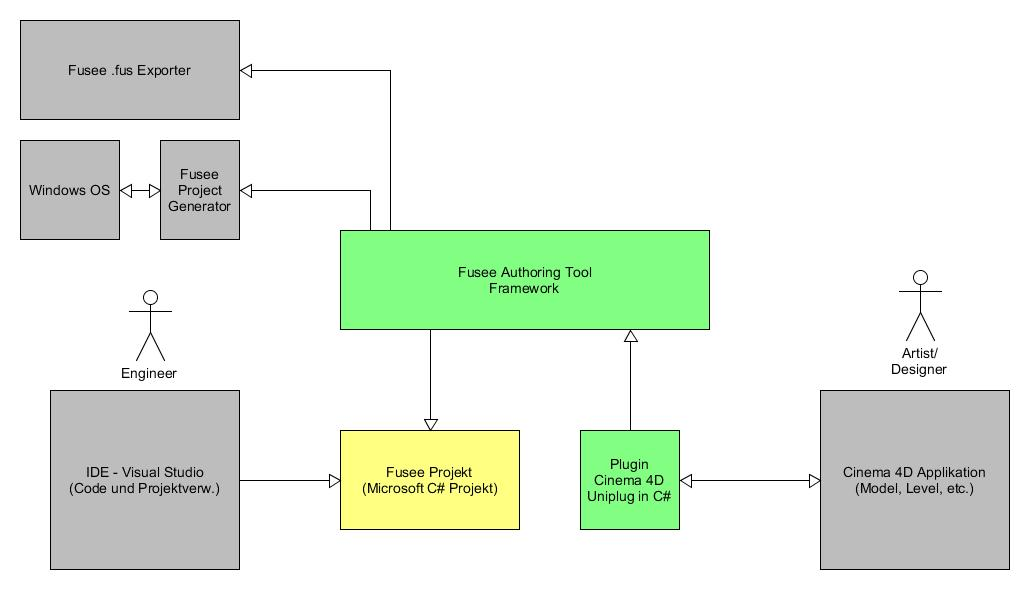
\includegraphics[width=\linewidth]{Bilder/Ueberblick_System.jpg}
	\caption{Überblick über die Systemarchitektur}
	\label{FuseeATSystemÜberblick}
\end{figure}
Das gelb hinterlegte Fusee Projekt beschreibt ein sich in Produktion befindliches Engine Projekt. Im Unterschied zu den aktuell meisten Fusee Projekten verwendet es allerdings für den Verlauf dieser Arbeit einen Binary Build der Engine. Dies hat den Vorteil, dass nicht der komplette Engine Code während der Arbeit für ein einziges Projekt mitgetragen werden muss. Der Engine Code direkt, wird während dieser Arbeit nicht erweitert, sie beschränkt sich lediglich auf die Erweiterung des Uniplug Projektes welches hier im Plugin Cinema 4D Uniplug in \CSS Container dargestellt ist. Das Uniplug Projekt ist nicht direkt im Kern der Engine angesiedelt und lässt sich deshalb getrennt von dieser bearbeiten.
\\
\\
Damit das System erfolgreich arbeiten kann ist es nötig, aus Cinema 4D verschiedene Information an das FuseeAT zu übertragen. So muss im Plugin zu Cinema 4D ein Fusee Projekt geöffnet werden. Dies kann über einen UI Dialog geschehen, der die vom Benutzer eingetragenen Informationen über den Projektort auf der Festplatte des Nutzers dann an das FuseeAT weiterleitet. Somit kann das FuseeAT dann die komplette Steuerung des Projektes übernehmen und Cinema 4D stellt nur eine Benutzerschnittstelle zur Interaktion dar. Somit wäre jegliche Funktionalität des FuseeAT in das eigentliche Authoring Framework ausgelagert und somit vom Programm Cinema 4D (oder anderen) abgekoppelt und unabhängig. Das Cinema 4D Plugin, in der Abbildung \ref{FuseeATSystemÜberblick} ebenfalls in grün dargestellt, stellt also nur die Schnittstelle des FuseeAT zur Software Cinema 4D dar und dient in diesem Fall als Kommunikationssystem zwischen den verschiedenen Architekturen C++ und \CS.


\subsection{Systemdesign für ein Tool Framework}
Die folgende Abbildung \ref{FrameworkÜberblick} zeigt das Design für das FuseeAT im Überblick. Der grau hinterlegte Container steht für die mit Hilfe des Uniplug Projektes zu entwickelnde Cinema 4D API Benutzer Schnittstelle. Das FuseeAT kann in vier Bereiche aufgeteilt werden. Zuerst einmal wäre hier das Schnittstellen Modul des FuseeAT für die Kommunikation mit einem Plugin das außerhalb des Systems verankert ist. Dieses FuseeAT Modul nimmt jegliche Calls (z. Dt. Aufrufe) entgegen und wandelt sie in Operationen des FuseeAT um. Hierzu verwendet weitere Module. Zu den Modulen gehören:
\begin{itemize}
\item FuseeAT Projekt Manager
\item FuseeAT File I/O Manager
\item FuseeAT Build Manager
\end{itemize}

\begin{figure}[ht]
	\centering
	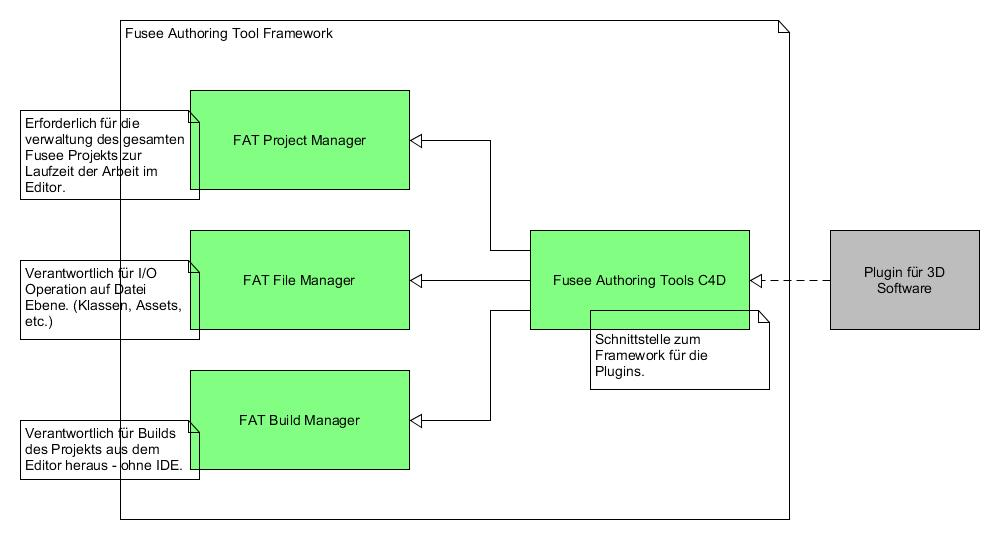
\includegraphics[width=\linewidth]{Bilder/Ueberblick_Framework.jpg}
	\caption{Überblick über das Fusee Authoring Toolkit Framework}
	\label{FrameworkÜberblick}
\end{figure}

Diese Module teilen sich die Aufgaben des FuseeAT. Der Projekt Manager behandelt hierbei jegliche Aufgaben die im Zusammenhang mit der Verwaltung, zur Laufzeit,  eines FuseeAT (bzw. Fusee Engine) Projektes stehen.
Das Modul FuseeAT File Manager ist ein Modul welches sich um jegliche I/O (kurz für Input Output) Operationen kümmert. Hier werden Tasks auf Betriebssystem Dateiebene erledigt. Dazu gehört beispielsweise das Erstellen und das Speichern von Dateien. Dieses Modul kann weiterhin für das anlegen von \CSS Klassen im Bereich der Programmierung zuständig sein und somit die Verbindung zwischen Assets und Code herstellen können.
Der FuseeAT Build Manager ermöglicht das Bauen eines \CSS Projektes durch Verwenden des von Microsoft bereitgestellten MSBuild\footnote{\url{https://msdn.microsoft.com/en-us/library/0k6kkbsd.aspx}} Systems. Er kümmert sich um Ausgabeverzeichnisse und weitere Optionen die während eines Buildprozesses Angaben des Benutzers benötigen. Der Buildprozess könnte durch die Plugin Kommunikation direkt aus Cinema 4D heraus angestoßen werden um das Fusee \CSS Projekt zu erstellen.

Das Klassendiagramm in Abbildung \ref{FuseeATKlassendiagramm} beschreibt in einer Detaillierteren Variante das FuseeAT. Die einzelnen Module sind hier in Klassen aufgeteilt und ein Teil der benötigten Methoden ist enthalten. Das Interface FuseeATBase (hier in Gelb hinterlegt) bildet die Ausgangsposition. Es bietet dem Cinema 4D Plugin System die Möglichkeit mit dem FuseeAT zu kommunizieren. Das FuseeAT wurde so designed, dass es Softwareunabhängig implementiert werden kann. FuseeATCinema 4D implementiert dieses Interface und verteilt die Aufgaben weiter an den ProjektManager. Dieses Modul kommuniziert selbst mit dem FileManager und dem BuildManager um die gewünschten Operationen zur Laufzeit zu erledigen. Das FuseeATCinema 4D Modul erhält Rückmeldungen über die return Werte der aufgerufenen Funktionen und kann somit dem Plugincode Rückmeldung über den Erfolg einer Aktion geben. Somit ist es möglich einem Benutzer in gewisser Weise ein Feedback zu seiner gerade ausgeführten Operation zu geben. Bei diesen Operationen könnte es sich z.B. um das Anlegen einer Datei, oder das Öffnen eines Projektes handeln.
\begin{figure}[ht]
	\centering
	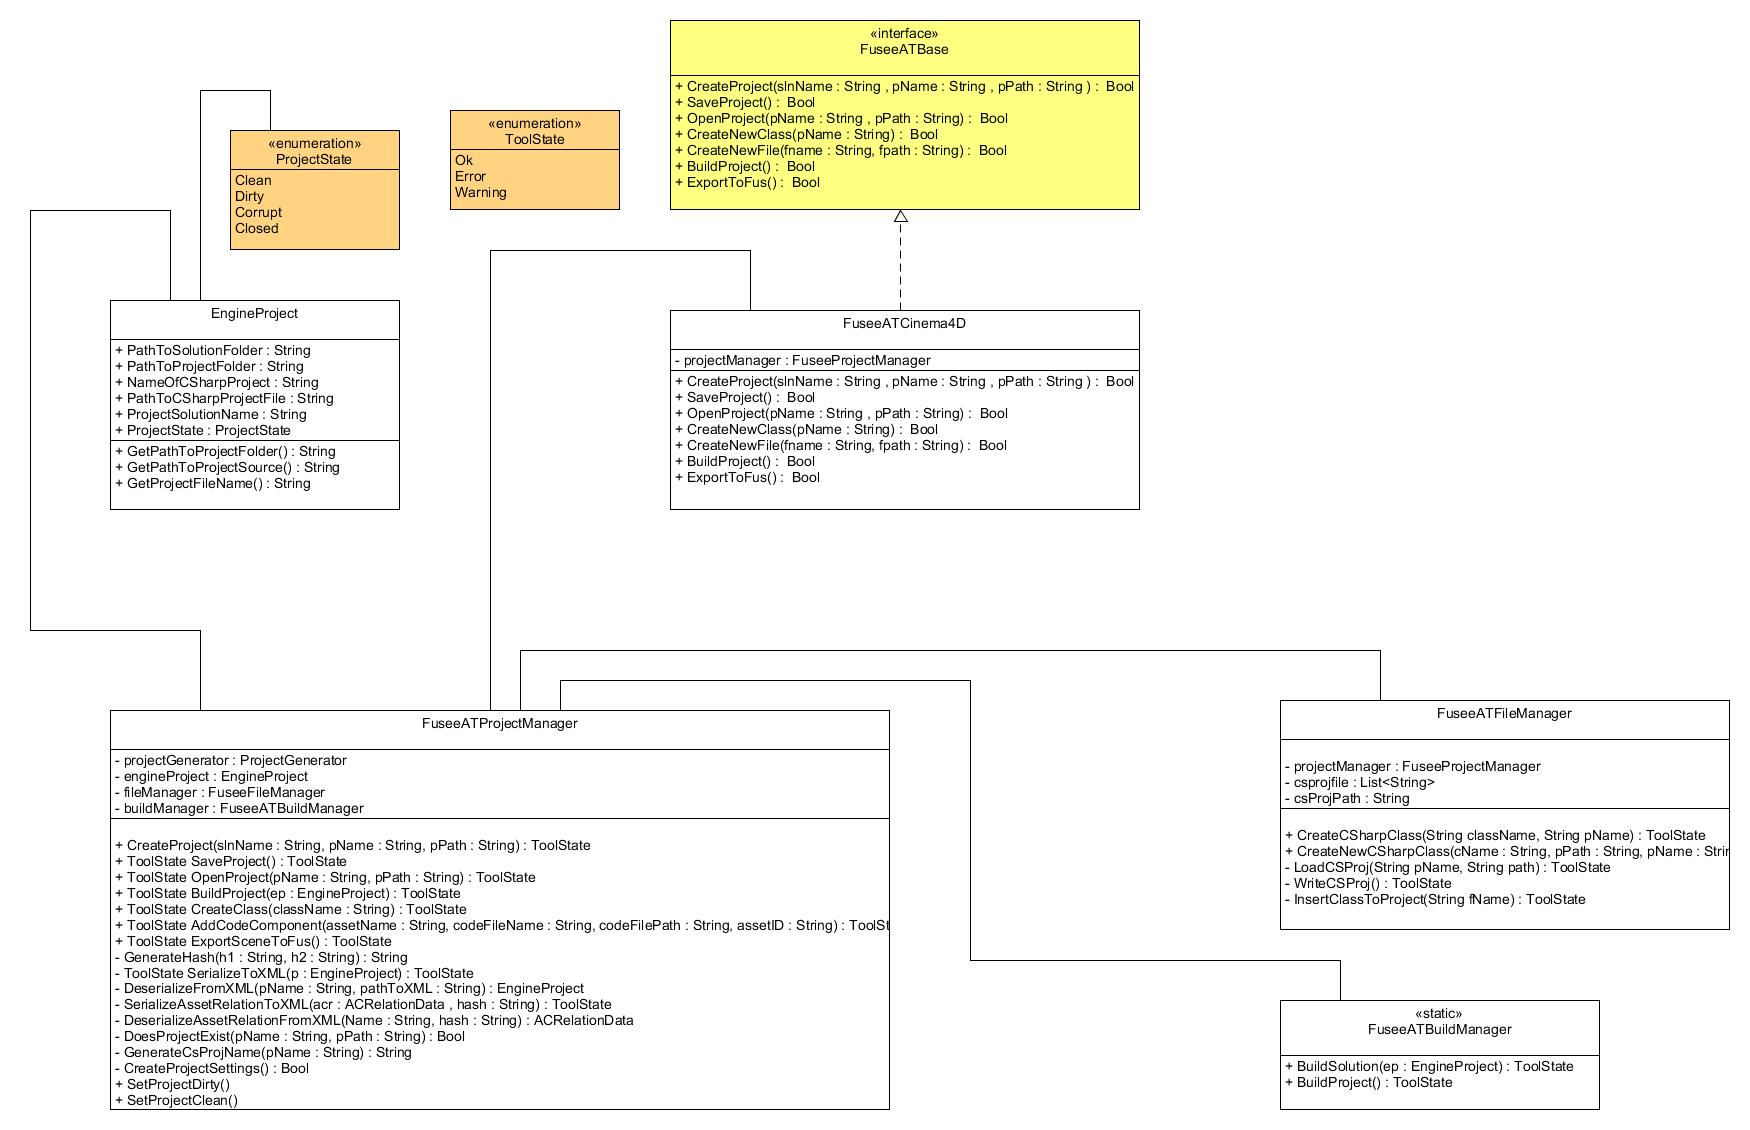
\includegraphics[width=\linewidth]{Bilder/Klassendiagramm_FuseeAT.jpg}
	\caption{Klassendiagramm für das Fusee Authoring Toolkit}
	\label{FuseeATKlassendiagramm}
\end{figure}
Das Klassendiagramm \ref{FuseeATKlassendiagramm} zeig bereits die Kompositionen der einzelnen Klassen auf. Die beiden Enumerationen ProjectState und ToolState (in Orange hinterlegt) dienen dazu die Integrität eines Fusee Engine-Projektes zu jeder Zeit zu gewährleisten. Sie werden als Rückgabewerte der Schnittstellen Funktionen nach außen eingesetzt und können somit einen möglichen Entwickler, welcher das FuseeAT erweitern möchte, darüber Informieren ob eine Aktion erfolgreich war oder nicht. Der Entwickler kann dann entscheiden, wie er mit der gewonnenen Information umgehen möchte. In manchen Situationen würde es Sinn machen auf diese Information, evtl. mit einen Rollback oder Ähnlichem zu reagieren. Hier sei angemerkt, dass sich mit dem vormals erwähnten ATF Framework von Sony ein solches Do und Undo System in \CSS realisieren ließe. Es bietet laut Dokumentation ein solches System zur Integration an.


\subsection{Systemdesign für ein Plugin System}
Die Abbildung \ref{ÜberblickPluginArchitektur} bietet einen Überblick über das Design des Uniplug Teil des Projektes. Damit verschiedene Funktionen in Cinema 4D angeboten werden können, benötigt das gesamte System verschiedene Arten von Plugin Typen. Das CommandPlugin designed zum öffnen, bauen und speichern eines Projektes. Es wird vom Benutzer durch den Aufruf eines Dialogs im Cinema 4D Plugin Menü gesteuert.

\begin{figure}[ht]
	\centering
	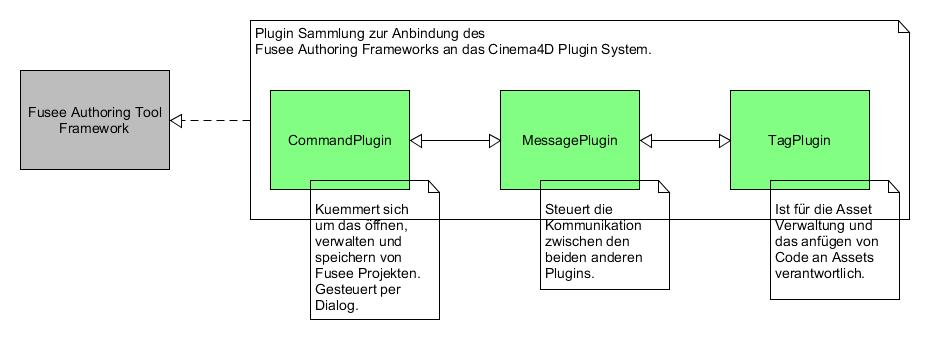
\includegraphics[width=\linewidth]{Bilder/Ueberblick_Plugins.jpg}
	\caption{Überblick über die Pluginarchitektur}
	\label{ÜberblickPluginArchitektur}
\end{figure}

Das TagPlugin kümmert sich um die Zuordnung von Assets. Es ermöglicht es in Cinema 4D so genannte Tags, welche Informationen in verschiedenen Formen speichern können, an ein 3D Objekt zu heften (in Form eines Icons im Szenengraphen) und so eine Verbindung zwischen Code und Content herzustellen.
\begin{figure}[ht]
	\centering
	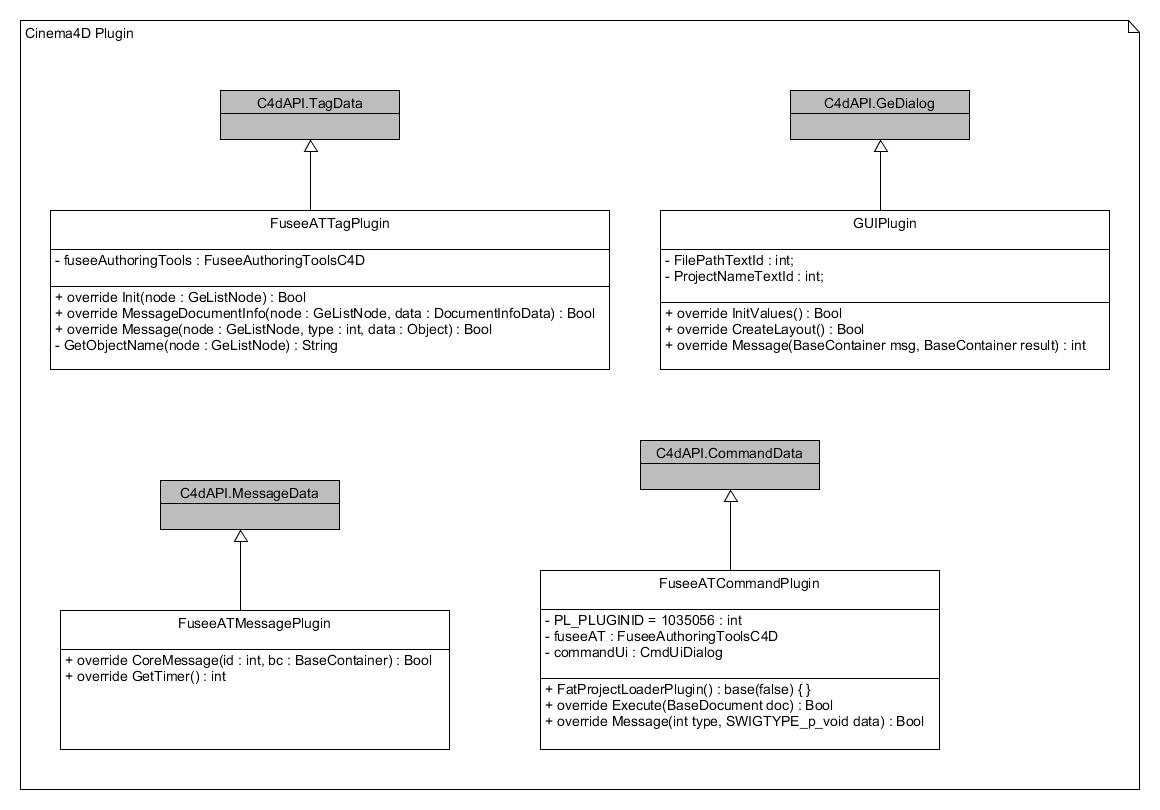
\includegraphics[width=\linewidth]{Bilder/Klassendiagramm_Plugin.jpg}
	\caption{Klassendiagramm der Plugin Architektur}
	\label{KlassendiagrammPluginArchitektur}
\end{figure}
Das MessagePlugin ist ein Hilfsplugin und implementiert keine Funktionalität sondern unterstützt die per Nachrichtensystem gesteuerte Kommunikation innerhalb von Cinema 4D. Durch dieses Plugin können Nachrichten des CommandPlugin an das TagPlugin und umgekehrt versandt werden. Die Nachrichten werden dann in den jeweiligen Plugins geparsed (sie bestehen aus einer Integer ID und einem Datenanteil\footnote{Von der Cinema 4D API festegelegt.}) und weiter verarbeitet. 
Das hier angeführte Klassendiagramm \ref{KlassendiagrammPluginArchitektur} zeigt die für jedes Plugin benötigten API Funktionen. Diese Funktionen müssen im Plugin Code als überschriebene Funktionen implementiert werden. Die Klasse GUIPlugin implementiert ein UserInterface um ein Fusee Projekt von Cinema 4D aus über einen Grafischen UI Dialog zu laden.

\subsection{Zeitersparnis durch das Verwenden von Fusee Modulen}
Um nicht jegliche Funktionen neu implementieren zu müssen, wurde vor dem Beginn der Implementierung geprüft welche Funktionalitäten bereits in der Fusee Engine gegeben sind. Durch die offene Struktur der Engine konnte bereits früher schon Code wiederverwendet werden. Diese Synergien der bereits vorhandenen Systemen sollten auch in zukünftigen Entwicklungen genutzt werden um, Zeit und Ressourcen zu sparen.
Die folgende Module des Fusee Projekts wurden für den Rahmen dieser Arbeit angepasst und verwendet.

\subsubsection{Der Fusee Projekt Generator}
Der Fusee Project Generator ist ein Projekt das bereits vom ersten Fusee Entwicklerteam angestoßen wurde. Es  handelt sich hierbei um ein Bibliotheksmodul welches es ermöglicht, ein neues \CSS Projekt innerhalb einer Fusee Solution anzulegen. Im Rahmen dieser Arbeit wurde der Fusee Projekt Generator lediglich neu innerhalb des Uniplug Projektes verdrahtet. Davor war der Generator noch eine eigenständige Konsolen .Exe Anwendung. Aktuell können mehrere Projekte mit ein und dem selben Engine Binary Build gebaut und verdrahtet werden. Die folgende Abbildung \ref{FuseeBinaryProjektStruktur} zeigt die Struktur eines solchen Fusee Projektes.
\begin{figure}[ht]
	\centering
	\includegraphics[width=\linewidth/2]{Bilder/FuseeBinaryProjekt.jpg}
	\caption{Fusee Binary Projekt Struktur}
	\label{FuseeBinaryProjektStruktur}
\end{figure}
 Die Solution Datei beinhaltet die zwei Projekte “Simple” und “TestProjekt”. Diese Projekte beherbergen in den Referenzen jeweils die Binary Bibliotheken der Fusee Engine. Das Projekt TestProjekt wurde mit dem Fusee Generator angelegt. Hierfür benötigt der Generatur nur den gewünschten Namen des Projekts und den Pfad zum Fusee Binary Projekt auf der Festplatte des Benutzers.



\subsubsection{Fusee .fus Exporter}
Beim Fusee Exporter handelt es sich um ein von Herrn Prof. C. Müller (Hochschule Furtwangen, Fakultät Digitale Medien) entwickeltes Cinema 4D Plugin. Das Plugin wurde ebenfalls mit Hilfe des Projektes Uniplug entwickelt. Es ermöglicht das exportieren einer Cinema 4D Szene in ein von Fusee lesbares Format (.fus). Dieses binary Format lässt sich in Fusee direkt im Code einer Engine Applikation laden und enthält sowohl Geometrie als auch weitere Bestandteile wie z.B. Materialien. Das Systemdesign sieht vor, dieses Plugin in das FuseeAT zu integrieren. Es erfüllt die Aufgabe des exports von Model bzw. Szenendateien in das Fusee Format zufriedenstellend und muss für eine Implementierung noch aus der Form eines Plugins in die Form einer Softwarebibliothek gebracht werden. Der Fusee Exporter ist an Cinema 4D gebunden und kann daher lediglich für den Export aus Cinema 4D genutzt werden. Für eine Verwendung in anderen Programmen müsste eine Schnittstelle geschaffen werden. Der Fusee Exporter operiert direkt auf den von Maxon in der API bereitgestellten Datentypen und Methoden einer Cinema 4D Szene.
Das Plugin bietet weiterhin die Möglichkeit eine Szene aus Cinema 4D in eine im Web Browser lauffähige Version einer Fusee Szene zu exportieren. Dies geschieht mittels der Verwendung von JSIL und verschiedener Javascript Bibliotheken. Weitere Informationen finden sich im Wiki\footnote{Fusee Wiki zum Web Export: \url{https://github.com/FuseeProjectTeam/Fusee/wiki/HowTo:-Fusee-on-Web}} zu Fusee.

\section{Asset Management und Asset Pipeline in der Fusee Engine}
Da sich die Fusee Engine in stetiger Entwicklung befindet, gibt es bis jetzt noch keine gesondert etablierte Asset Management Pipeline. Assets werden bis jetzt in Visual Studio direkt im Code per Include eingebunden. Genau so wie alle Fusee Projekte ohne grafische Oberfläche in Visual Studio erstellt werden müssen. Meist handelt es sich bei in Fusee eingebundenen Assets um eines der folgenden Asset-Typen:
\begin{itemize}
\item 3D-Modelle in den Formaten .obj\footnote{Weitere Informationen zum Format unter: \url{http://www.fileformat.info/format/wavefrontobj/egff.htm} Online: geprüft am 27.04.2015} (Bei dem Dateiformat handelt es sich um das lesbare ASCII Model Datenformat “Wavefront Object”\footnote{Entwickelt von Wavefront, das Unternehmen war später unter dem Namen Alias bekannt und wurde zwischenzeitlich von Autodesk aufgekauft \url{http://www.autodesk.de/}})
\item 2D-Texturen in den Formaten (JPEG, JPG, PNG)
\item Audio Datei im Format Wav, Ogg, etc. (Unterstützt alle von der SFML “Simple and Fast Multimedia Library \url{http://www.sfml-dev.org/} unterstützen Formate.
\end{itemize}


\subsection{Asset Pipelines in Fusee Authoring Toolkit}
Die folgende Grafik \ref{FuseeATAssetIteration} \footnote{Abbildung entnommen aus \cite[S. 7]{Carter2004} und neu Illustriert und beschriftet.} ergänzt die Erläuterung zum Asset Authoring (Eines .fus Objektes mit angehängtem Code Component\footnote{Ein Extra Element welches an einem Asset Objekt angehängt ist} oder anderen) mit Hilfe der Asset Pipeline während der Produktion eines Fusee Engine Projektes. Hierbei handelt es sich um einen iterativen Prozess welcher je nach Ergebnis des Tests und der Evaluation im Engine Projekt eine neue Iteration des Prozesses nach sich ziehen kann. In der Grafik \ref{FuseeATAssetIteration} wird Beispielhaft ein Model in Cinema 4D erstellt, ein Component angehängt und anschließend vom FuseeAT System zur Laufzeit zu einer XML Datei serialisiert. Diese XML Datei kann dann von jedem Entwickler editiert werden. Die Datei wird weiterhin von FuseeAT in der Cinema 4D Szene benötigt um eine Zuordnung eines Asset in der Szene wiederherzustellen.
Das erstellte Asset bleibt weiterhin im Cinema 4D Format, gespeichert in der Cinema 4D Datei des Projektes, vorhanden. Somit besteht das Asset in einer nativen Version weiterhin und kann in einem iterativen Prozess weiterhin verändert werden.

\begin{figure}[ht]
	\centering
  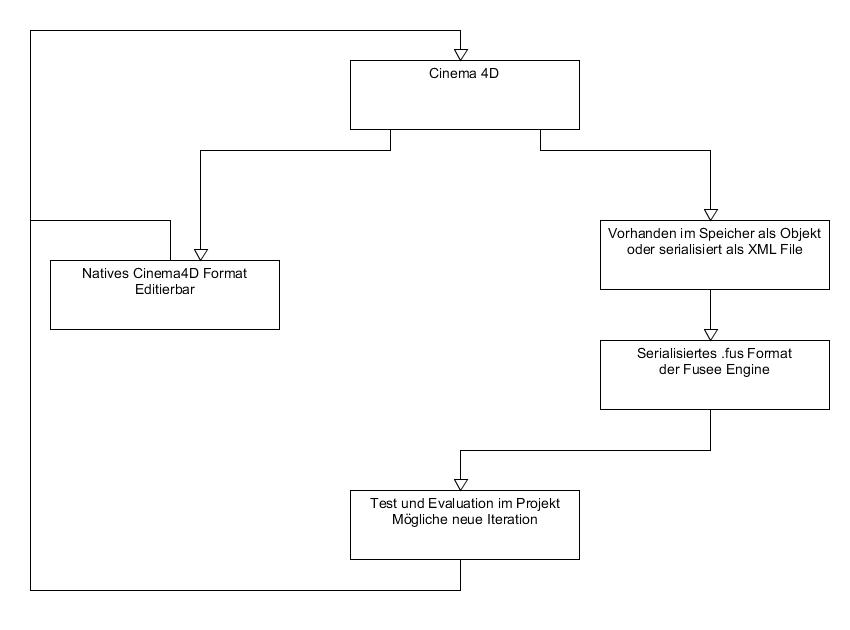
\includegraphics[width=\linewidth]{Bilder/FuseeATAssetPipeline.jpg}
	\caption{Asset Loop während der Produktion eines Projektes in Fusee und FuseeAT}
	\label{FuseeATAssetIteration}
\end{figure}

Während des Build- und/oder Speichervorgangs des Cinema 4D und Fusee Projekts über das FuseeAT wird das Asset vom Framework in ein Asset des Fusee Typs .fus gewandelt. Allerdings geht durch die bereits erwähnte redundante Speicherung des Asset im Cinema 4D Format keine Information der ursprünglichen Datei verloren.

\subsection{Assetmanagement in Fusee Authoring Toolkit}
Oft reicht eine einfache Versionierung, durch z.B. Git, von binären Asset Dateien wie Texturen oder Modellen nicht aus und muss daher von geeigneteren Tools übernommen werden. Das Assetmanagement innerhalb eines Projektes wird von FuseeAT nicht abgedeckt und sollte vom Entwicklerteam übernommen werden. Hierzu können verschiedene Tools eingesetzt werden die auf ein Management von Binary Asset Files spezialisiert sind. Beispiele für solche Systeme sind die Software Alienbrain \autocite{Alienbrain}\footnote{Webadresse: \url{http://www.alienbrain.com/}} und die Software Shotgun \autocite{Shotgun}\footnote{\url{https://www.shotgunsoftware.com/}}. Diese kommerziellen Tools erlauben das Verwalten von Binären Assets (z.B. Audio Dateien, 3D-Modelle, Grafiken) während der Produktion von Entertainment Produkten. Eine solche Software kann ohne Probleme neben dem FuseeAT eingesetzt werden, da sich die beiden Wirkungsbereiche nicht überschneiden.
Da FuseeAT jedoch auf human readable file formats setzt und diese als XML Dateien im Projekt Ordner ablegt, kann für die Versionierung von FuseeAT Projekten ein VCS wie Git herangezogen werden. Ein weiterer Vorteil der lesbaren XML Dateien ist der unkomplizierte Merge-Vorgang innerhalb des VCS, Bei Problemen können Entwickler diese Dateien auch jederzeit von Hand verändern und das Projekt in Cinema 4D erneut laden.

\chapter{Umsetzung des Konzeptes}
\section{Die Cinema 4D C++ API und deren Verwendung in diesem Projekt}
Für die Implementierung in Fusee und dem Cinema 4D Pluginsystem war es nötig, auf das Uniplug System der Hochschule Furtwangen \footnote{Entstanden durch die Leitung und Entwicklung von Herrn. Prof. C. Müller, Fakultät Digitale Medien, in ständiger Weiterentwicklung durch Mitglieder und Studierende des Fusee Teams.} zurückzugreifen. Damit das Uniplug System in dieser Arbeit genutzt werden konnte, waren einige Erweiterungen nötig. Da dies einen erheblichen Zeitaufwand vor und während der Implementierung bedingte und eine Abhängigkeit von FuseeAT darstellt, soll hier darauf eingegangen werden.

\subsection{Ausgangssituation und in der Implementierung verwendete Softwareprojekte}
Das Projekt “Fusee Authoring Toolkit” \footnote{Der Name der zu dieser Arbeit zugehörigen Softwarebibliothek.} (kurz: FuseeAT) basiert auf mehreren Software Projekten. Ein Teil dieser Projekte wurde an der Hochschule Furtwangen entwickelt. Ein anderer Teil stammt von externen Entwicklen und gehört zu proprietärer Software. Dieser Abschnitt gibt einen Überblick über die verwendeten Softwarebestandteile und ihrer Einbindung in der Implementierung zur Zeit dieser Arbeit.
\\
\\
Verwendet wurden:
\begin{itemize}
\item Fusee Math Bibliothek, eine von Fusee unabhängige Sammlung in \CSS geschriebener Mathematischer Funktionen und Datentypen
\item Uniplug, ein in Fusee beinhaltetes Projekt zum Schreiben von Plugins in \CSS für Cinema 4D
\item Die Fusee Engine, eine Interaktive Simulations Engine zur Darstellung zweidimensionaler und dreidimensionaler Szenen
\item Die Maxon Cinema 4D API(Hier sind nur C++ Headerfiles verfügbar. Jeglicher implementierter Cinema 4D Programmcode ist nicht einsehbar.)
\item Verschiedene Windows Bibliotheken aus dem .NET Framework auf welche hier nicht weiter eingegangen werden soll
\end{itemize}

\subsection{Cinema 4D Plugin API und SDK}
Cinema 4D R16 \autocite{MaxonC4d2014} ist ein kommerzielles proprietäres Produkt des Unternehmens MAXON Computer GmbH und steht nicht als Open Source Projekt zur Verfügung. Maxon stellt daher für die Entwicklung von Plugins\footnote{Plugins in C4D - Erweiterungen für die Software Cinema 4D und deren Funktionen} und die Erweiterung des Cinema 4D Funktionsumfangs eine API\footnote{Application Programming Interface, z. Dt. Programmierschnittstelle} bereit. Bei dieser API handelt es sich um eine Bibliothek geschrieben in C++. Dieser Code kann in Form von Header Files in die eigene Applikation integriert werden. Durch diese C++ Headerfiles ergibt sich eine Schnittstelle zu internen Methoden in der Cinema 4D Software. Die tatsächliche Implementierung kann mit der API nicht eingesehen werden, es handelt sich hier lediglich um Header Files ohne den tatsächlichen Code. Das C++ SDK wird bei einer Installation von Cinema 4D automatisch mit installiert. Auf einem Windows PC findet sich das SDK und die dazugehörigen Visual Studio Solution Dateien unter folgendem Pfad ausgehend vom Installations Ordner der 64Bit Version von C4D\footnote{Cinema 4D liegt seit der Version R15 nur noch als 64 Bit Version vor und benötigt laut \url{http://www.maxon.net/?id=311}(Maxon C4D System Requirements) ein 64 Bit System}: {“Cinema 4D/plugins/cinema4dsdk”}.
\\
Maxon bietet Beispiele zur Cinema 4D API auf einem GitHub Account\footnote{\url{https://github.com/PluginCafe}} unter der Apache License Version 2.0, January 2004\footnote{Apache Licence 2.0 \url{https://github.com/PluginCafe/cinema4d_cpp_sdk/blob/master/LICENSE}} zum kostenfreien Download an. Das C++ SDK/API ist seit der Version R16 fester Bestandteil der Cinema 4D Installation und muss nicht extra heruntergeladen oder gebaut werden.

Voraussetzung für das Erstellen eines Plugins ist, dass der eigene Plugin Code laut Maxons Dokumentation einige Funktionen überschreiben bzw. Klassen vererben muss. Ansonsten ist der Inhalt des Quellcodes seitens Maxon nicht beschränkt. Das folgende Schaubild \ref{C4D API Schaubild} erläutert die Funktionsweise des Cinema 4D Plugin Systems. Der Entwickler kann seinen C++ Code fast frei entwickeln und ist nur dazu angehalten sich an Maxons Richtlinien zur Kommunikation mit dem Produkt Cinema 4D zu halten. Der Entwickler hat dabei die volle Kontrolle über seinen eigenen Plugin Code. Die Schnittstelle (C4D API/SDK) ist zumindest durch die mitgelieferten C++ Headerfiles noch einsehbar. Dies unterstützt den Entwickler eines Plugins während des debuggens. Sobald Aufrufe die eigentliche Software Cinema 4D erreichen, ist das einsehen des Codes nicht mehr möglich. Was wie später noch erläutert im Falle von Uniplug zu einigen Problemen führen kann.

\begin{figure}[ht]
	\centering
  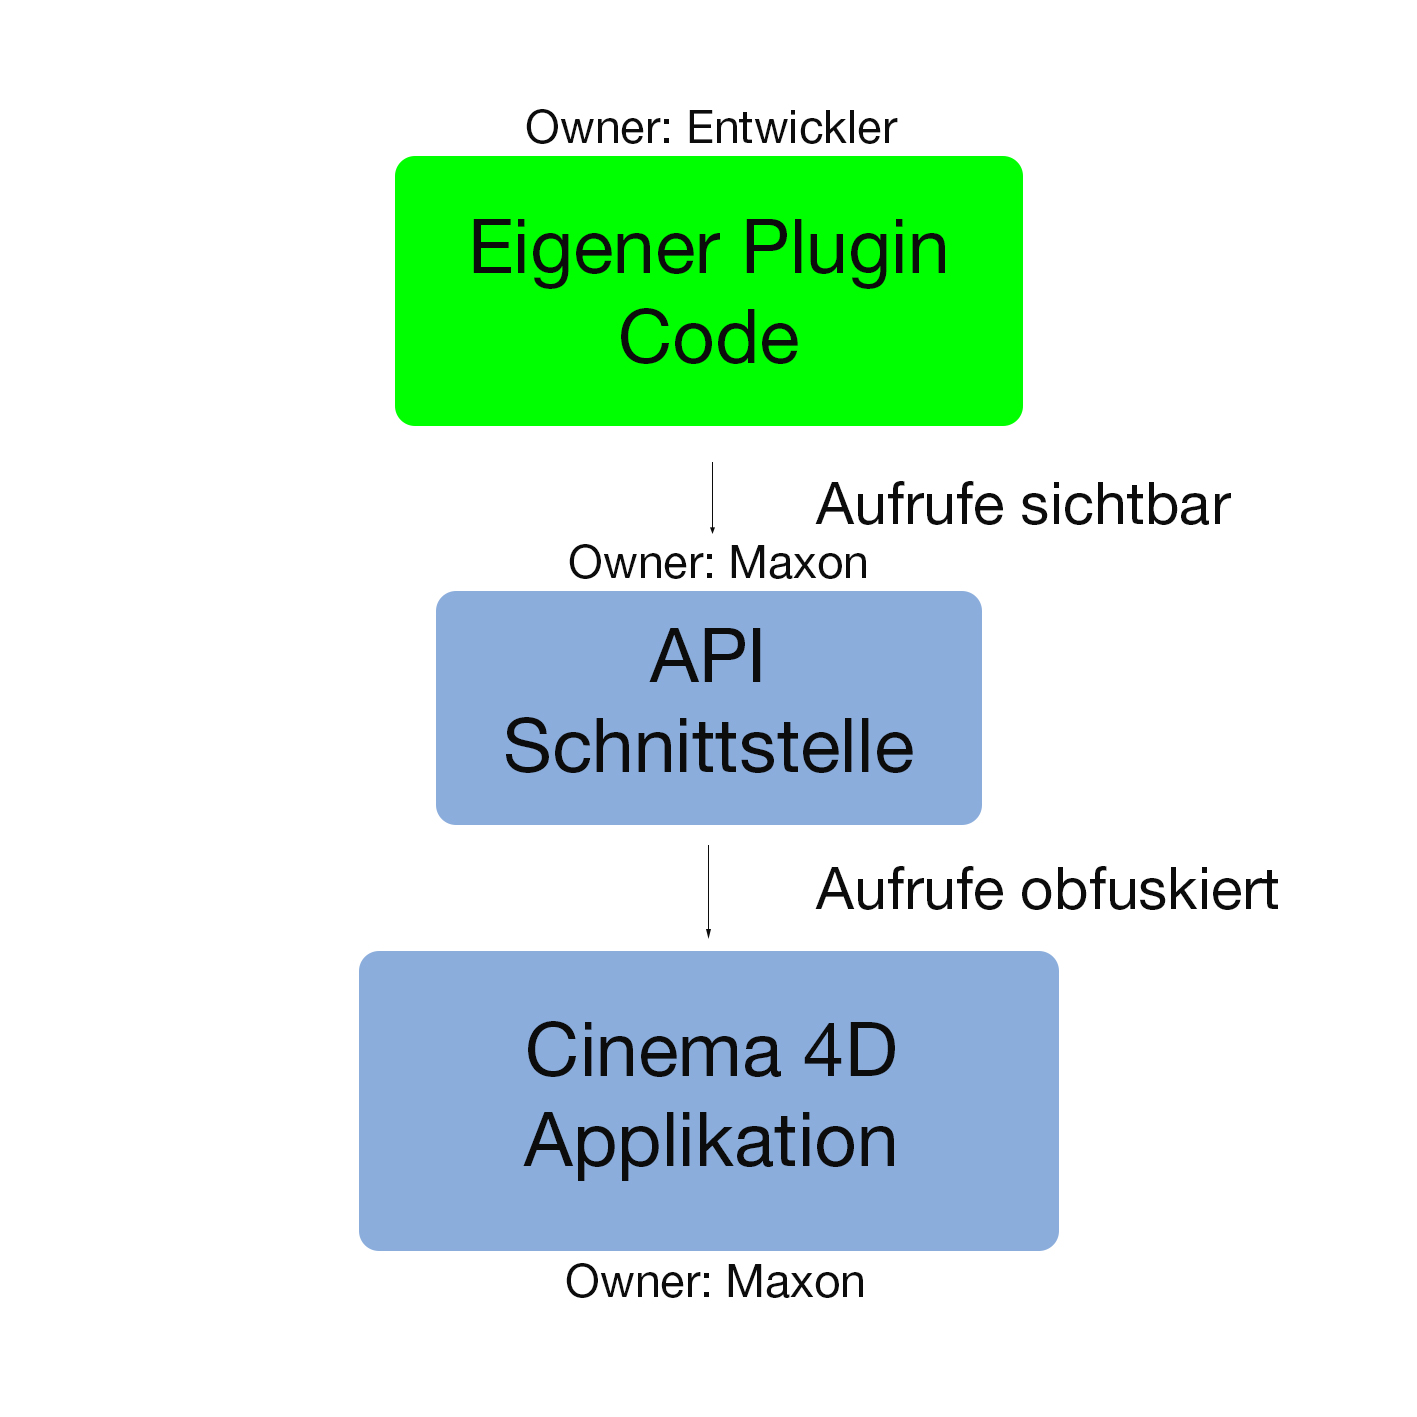
\includegraphics[width=\linewidth]{Bilder/C4D_Api_Schaubild_v1.jpg}
	\caption{Schaubild des Cinema 4D API Systems}
	\label{C4D API Schaubild}
\end{figure}

Das hier dargestellte Minimalbeispiel \ref{BasicC4dPlugin} in C++ Code zeigt ein einfaches minimalistisches Plugin welches beim Ausführen nur eine Ausgabe auf der Konsole von Cinema 4D erzeugt.

\newpage
\lstinputlisting[language=C++, caption = Einfaches Cinema 4D Plugin in der Programmiersprache C++, label=BasicC4dPlugin]{Code/minimalbeispielPlugin.h}
Dieser Code ist ein Wichtiger Bestandteil der Cinema 4D API und letztendlich auch des FuseeAT. Das Beispiel wird im nächsten Abschnitt relevant. Es folgt ein Überblick über das Uniplug Projekt welches das Schreiben von Cinema 4D Plugins mit Hilfe der Programmiersprache \CSS ermöglicht. Die oben gezeigte  Codestruktur wird dann noch einmal als \CSS Version erläutert.

\subsection{Uniplug}
Bei Uniplug handelt es sich um ein Teil des Projektes Fusee der Hochschule Furtwangen. Uniplug bietet die Möglichkeit Cinema 4D Plugins in \CSS zu schreiben. Hierfür bedient es sich eines Interface Compilers SWIG [\fullcite{SWIG2015}]. Das gesamte Uniplug Projekt ist ein Open Source Projekt und steht auf einem GitHub Repository unter \url{https://github.com/FuseeProjectTeam/Fusee} innerhalb des Fusee Projekts zum Download bereit. Das Uniplug Projekt stand bereits vor dieser Arbeit zur Verfügung. Allerdings hatte es nich den nötigen Umfang und das Projekt wurde während der Arbeit um wichtige Funktionen zur Entwicklung von Plugins erweitert. Folgende in Abbildung \ref{UniPlugVSStruktur} dargestellten Module sind Bestandteil des Uniplug Systems.

\begin{figure}[ht]
	\centering
  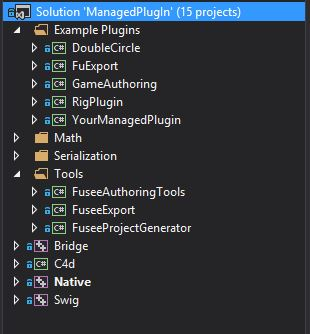
\includegraphics[width=\linewidth / 2]{Bilder/UniplugVSStruktur.JPG}
	\caption{Die Uniplug Projektstruktur in VisualStudio}
	\label{UniPlugVSStruktur}
\end{figure}
Die im Unterordner Tools aufgeführten Projekte sind das Kernelement dieser Arbeit. Es handelt sich dort um das FuseeAT. Das Plugin für die Cinema 4D Anbindung ist im Unterordner “Example Plugins” verortet und wird hier als “Game Authoring” bezeichnet. Es enthält jeglichen Plugin Code für diese Arbeit. Die Projektstruktur des UniPlug Projektes wurde während dieser Arbeit und dem Einfügen der neuen Funktionen weiter optimiert.

\subsubsection{Was ist SWIG?}
Bei SWIG handelt es sich um einen SoftWare Interface Generator. Swig unterstützt Entwickler dabei, eine Codebase aus z.B. einer nativen Programmiersprache wie C++ in eine managed Programmiersprache wie z.B. \CSS zu “übersetzen”. Hierbei handelt es sich allerdings nicht wirklich um einen übersetzungs bzw. Compilevorgang. Vielmehr unterstützt Swig den Entwickler durch das generieren spezifischer Interface Files welche die Aufrufe (calls) einer “externen” Software an den “gewarppten” Teil der Software weiterleiten. Die Ausgangssoftware wird also immernoch benötigt (im Falle von Uniplug) und auch verwendet (das Cinema 4D API Framework). Vgl \fullcite{SWIGIntroduction2015}.

Eine Vollständige Dokumentation des SWIG Projektes findet sich unter folgender Adresse: \url{http://www.swig.org/Doc3.0/index.html} geprüft, letzter Stand der Erreichbarkeit 15.04.2015.

Swig wird bereits erfolgreich in vielen Projekten eingesetzt. Unter anderem finden sich in der Liste das bekannte Version Control System Subversion, die 3D Engine Ogre bzw. PyOgre und die große Image Processing Bibliothek OpenCV. Die offizielle Liste der SWIG Nutzer findet sich unter \url{http://www.swig.org/projects.html} - geprüft am 15.04.2015.

\subsubsection{Wrapping von C++ Code nach \CSS mit SWIG}


Um aus dem C++ Code der Cinema 4D API aufrufbaren \CSS Code zu erzeugen sind verschiedene Schritte notwendig. Ein SWIG Projekt welches wie in Abbildung \ref{SWIGUniplug} im Uniplug Projekt verfügbar ist enthält eine C4dApi.i (interface) Datei.

\begin{figure}[ht]
	\centering
	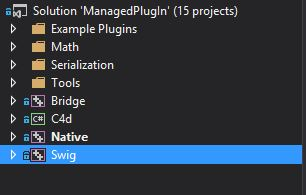
\includegraphics[width=\linewidth/2]{Bilder/ProjektstrukturSwig.JPG}
	\caption{SWIG im Uniplug Projekt (ManagedPlugIn) markiert durch blaue Selektion.}
	\label{SWIGUniplug}
\end{figure}

Diese Datei kümmert sich um das Wrappen des nativen C++ Codes nach \CS. Der eigentliche Wrapping Vorgang wird über ein SWIG make script aufgerufen welches während des Build Vorgangs des Projektes angestoßen wird. Dieser Vorgang muss bei der eigentlichen Plugin Entwicklung nicht bei jedem Build durchgeführt werden. Es genügt, die API erneut zu wrappen wenn Veränderungen am API Code seitens Maxon oder des Benutzers vorgenommen wurden. Änderungen durch den Benutzer schließen auch das Erweitern der API Funktionalität mit ein. Das Uniplug Projekt ist zum Zeitpunkt dieser Arbeit weit von einem Vollständigen Wrapping der Cinema 4D API entfernt. Aus diesem Grund, ist noch relativ häufig die Erweiterung des API Projektes nötig. Verschiedene Eintragungen die für das Erweitern des Uniplug Projektes vorgenommen wurden, werden im nächsten Abschnitt genauer erläutert. Hierzu gehören einfache Inklusionen von Source Files, aber auch komplexe overrides von bereits bestehenden C++ Funktionen.

Das hier abgebildete Schaubild zeigt den Ablauf des Wrapping-Vorgangs. Hierbei sind folgende Schritte zu erkennen:
\begin{itemize}
\item Erstellen des *.i Files und dortiges inkludieren der gewünschten nativen Code Dateien.
\item Erweitern von nativen Code Dateien um eigenen Nativen Code (nicht Zwangsweise nötig)
\item Überschreiben von nativen Code Dateien durch eigenen Nativen Code (nicht Zwangsweise nötig)
\item Kompilieren des SWIG Projektes durch Aufruf des Compilers.
\item Verwenden des kompilierten SWIG Codes in eigenen Projekten.
\end{itemize}

Die grauen Flächen im Diagramm beschreiben Aktionen in welche der Entwickler aktiv eingreifen muss. Das Interface File mit den gewünschten Dateien muss manuell geschrieben werden. Das erweitern oder überschreiben von Code muss ebenfalls manuell erfolgen. Der Aufruf des SWIG Compilers verläuft parallel zum Prozess des Erweiterns weil für eine Funktionsfähige wandlung des Codes keine Erweiterungen nötig sind. Es muss nur im Problemfall eingegriffen werden. Meist zeigt sich aber, dass in besonders komplexen Fällen, wie des wrappings der Cinema 4D API, doch recht häufig eingegriffen werden muss. Das Überschreiben (manuell) von Klassen und Methoden ist ein Optionaler Fall und wurde zum besseren Erkennen blau eingefärbt.
\begin{figure}[ht]
	\centering
	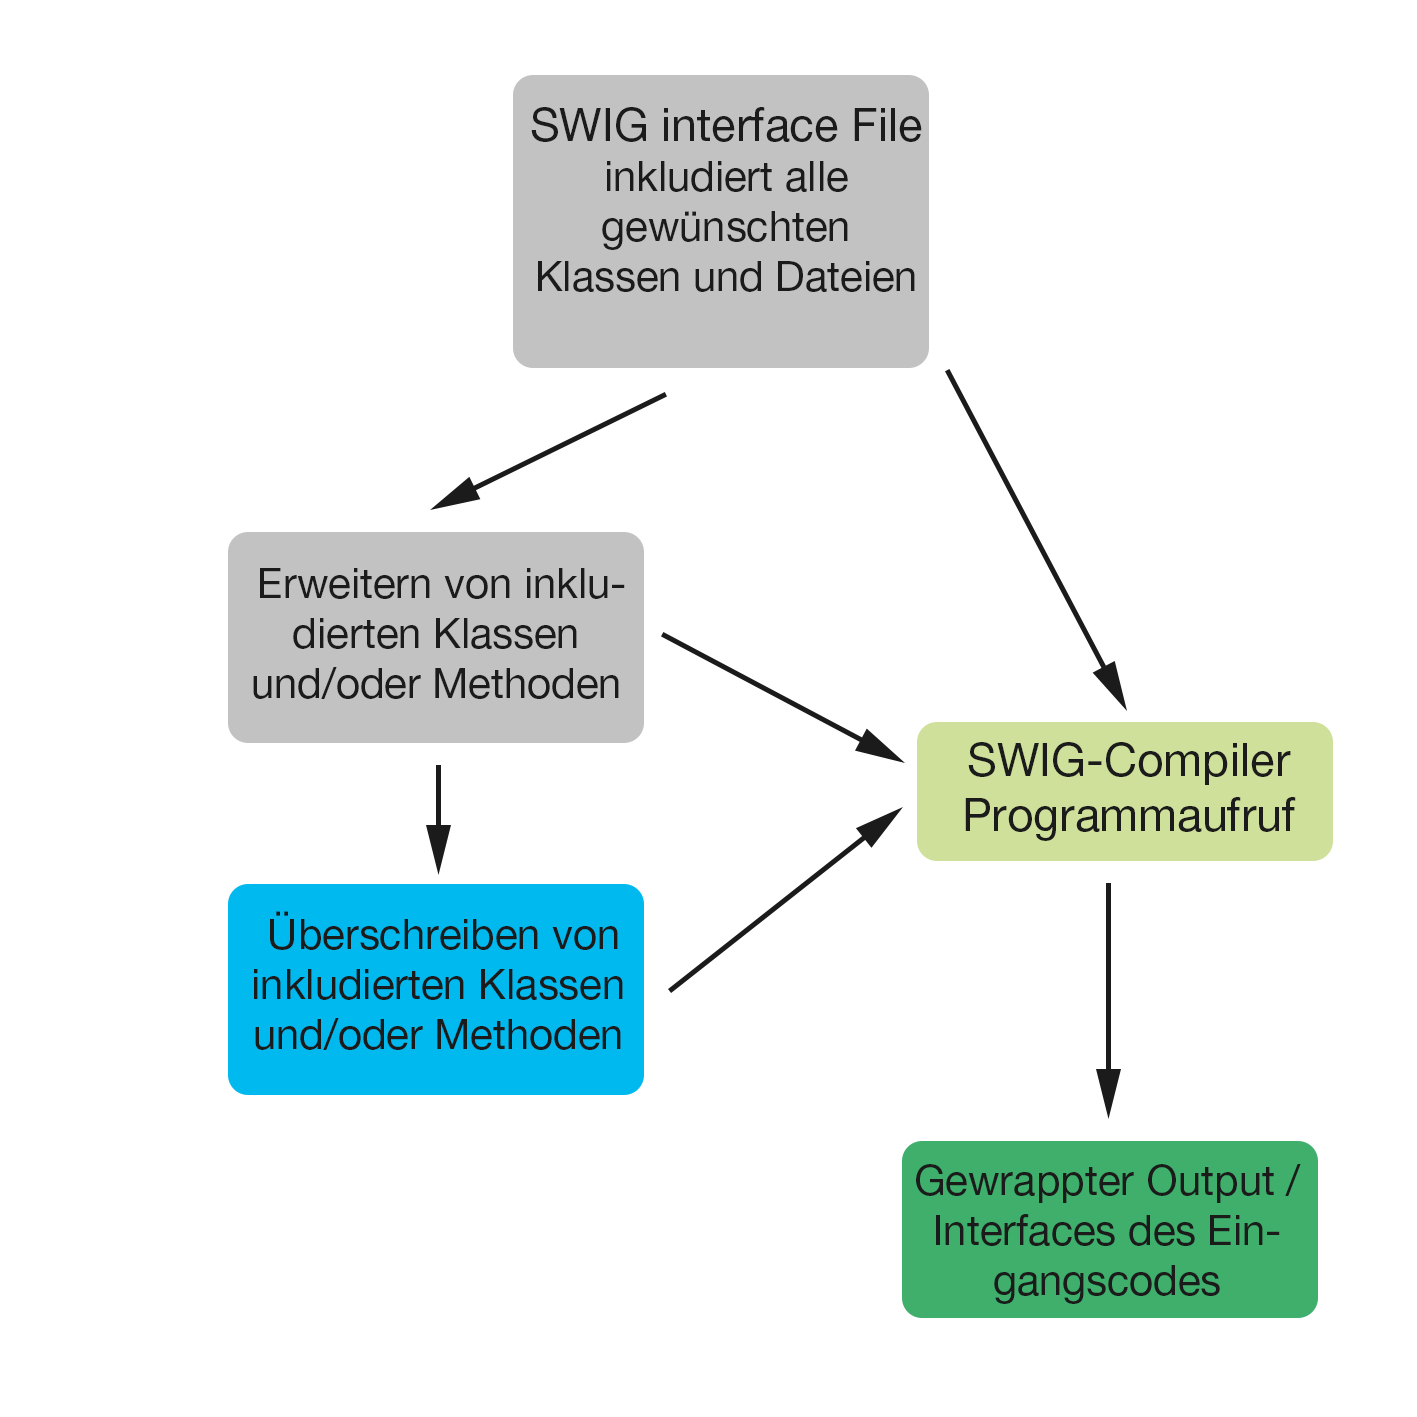
\includegraphics[width=\linewidth]{Bilder/swig_wrapping_csharp.jpg}
	\caption{Wrapping Vorgang der Cinema 4D API von C++ nach \CS}
	\label{SWIG wrapping Vorgang}
\end{figure}

\subsubsection{Erweiterung des Uniplug Codes für Plugins vom Typ TagPlugin}
Um das Projekt auf den Aktuellen Stand zu bringen und das schreiben des Plugins zu ermöglichen musste zuerst das Uniplug Projekt erweitert werden. Auch hier wurde mit iterativen Methoden gearbeitet. Falls Probleme mit verschiedene gewrappten Cinema 4D API Methoden auftragen, wurde zunächst geprüft, welche “pseudo” SWIG Dateien diese Probleme verursachten und welche Cinema 4D Api Funktionen aus diesem Grund in der \CSS API Code nicht vorhanden sind. Diese fehlenden Dateien wurden dann inkludiert und es wurde versucht das SWIG Projekt zu bauen. Sollte es bei diesem Schritt zu Problemen kommen, mussten die API Dateien genauer analysiert werden. In manchen Fällen war es nun nötig den nativen Code der API Dateien zu erweitern oder zu überschreiben. Bei der Implementierung des Cinema 4D Plugin Typs “TagPlugin” waren besondere Änderungen im API Code nötig. Hier sollen die Problematik und die Lösung dieser aufgezeigt und erläutert werden.
\\
\lstinputlisting[language=C++, caption = Einbinden des Maxon Cinema 4D C++ Datentyps TagPlugin in die \CSS API von Uniplug]{Code/c4dDataTypeToCSharp.h}

Um den Datentyp TagData korrekt im \CSS Code zu verwenden, waren noch weitere Anpassungen im Code notwendig. Die Methode Message() des TagData ElternTyps NodeData musste überschrieben werden um das Message System in \CSS nutzen zu können. Dies wurde nötig durch die Verwendung eines Void Pointers seitens Maxons in der Parameterliste der Message Funktion im C++ Code der API. SWIG kann an dieser Stelle durch den nicht auf einen Datentypen festgelegten Void Pointer des Datentyps der Parameterliste keine zufriedenstellende Wrappingfunktion bereit stellen. Das folgende Codebeispiel der Message() Funktion verdeutlicht den Fix im C++ Code des Uniplug Native Projektes.

Die Message() Funktion ist Teil eines Nachrichtensystems innerhalb von Cinema 4D. Viele Elemente des Programs und selbst geschrieben Plugins kommunizieren über dieses Messagesystem miteinander. Hierbei werden Messages über einen Broadcast versandt. Dieser Broadcast sendet in einer Parameterliste einen ID Code. ID Konstantenvon Cinema 4D werden meist als Konstante (mit define angelegte) Integer Variablen übergeben und können so in if else oder switch case Anweisungen vom Plugin Entwickler identifiziert und verarbeitet werden.

Im folgenden Code Beispiel sind einige dieser Konstanten dargestellt. Bei dem hier in Beispiel \ref{CodeMessageFunktion} abgebildeten Code handelt es sich um die überschrieben Message Funktion, welche die Verwendung des Systems für Plugins in \CSS erst möglich macht. Der void Pointer der Parameterliste wird während des Aufrufs der Funktion in andere Datentypen gecastet. Für die Wandlung der Message Funktion für die TagData Klasse war es von nöten ein Object des Typs DocumentInfoData zu erhalten. Aus diesem Grund, wird das Objekt dieses Typs bei einer bestimmten empfangenen Message ID zurück gegeben.
\begin{lstlisting}[language=C++, caption = Überschreiben der Message Funktion des TagData Datentyps, label=CodeMessageFunktion]
Bool TagDataM::Message(GeListNode *node, Int32 type, void *data)
{
	switch (type)
	{
	case MSG_EDIT:

		break;
	case MSG_GETCUSTOMICON:
		break;
	case COLORSYSTEM_HSVTAB:
		break;
	case MSG_DOCUMENTINFO:
		{
			DocumentInfoData* did = (DocumentInfoData*)data;
			return MessageDocumentInfo(node, did);
		}
		break;
	case MSG_DESCRIPTION_GETINLINEOBJECT:
		break;
	case DRAW_PARAMETER_OGL_PRIMITIVERESTARTINDEX:
		break;
	}

	return true;
}
\end{lstlisting}

Durch die eingeschränkte  Möglichkeit nur bis zum call des Debugging API Codes debuggen zu können (Hierzu mehr im Kapitel Probleme und Herausforderungen), war die Lösung des Problems nicht wie meistens in mit SWIG gewrappten Codebasen durch einen einfachen \%typemap\footnote{Ermöglicht das mappen eines Datentyps der Eingangssprache auf einen anderen Datentyp der Ausgangssprache} sondern nur durch die nachträgliche Implementierung der oben dargestellten switch case Anweisung innerhalb des Uniplug Projektes zu bewerkstelligen. 

\section{Der Fusee Szenengraph}
Wie bereits erwähnt, wird der Code der Fusee Engine für diese Arbeit nicht erweitert. Es wird im Systemdesign aber ein wichtiges Element der Engine, der Szenengraph, verwendet. Dieser Abschnitt geht auf die Funktionsweise des Szenengraphen in Fusee ein und zeigt seine Ähnlichkeiten und Unterschiede zum Szenenaufbau einer Cinema 4D Szene auf. 

Der Fusee Szenengraph ermöglich das Traversieren und Vorhalten verschiedener Elemente einer Fusee Szene. Der Graph ist aus einer Kombination von Nodes und Components aufgebaut. Er ähnelt stark dem Unity3D Ansatz des Szenengraphen. Eine Node ist ein Knotenpunkt ohne spezielle Daten. Die Node enthält lediglich einen Namen, eine Liste an Components und falls nötog, eine Liste an Kind-Nodes. Das Traversieren wird durch Visitor Implementierungen ermöglicht. Diese Visitor Patterns wurden während dieser Arbeit noch implementiert und erweitert. Ein Visitor ermöglicht das Traversieren einer Szene und seiner Nodes auf eine vom Entwickler definierte weise und kann so z.B. Transformationen durchführen, welche die Struktur einer Szene verändern.

\begin{figure}[ht]
	\centering
	\includegraphics[width=8cm]{Bilder/Fusee_Szenengraph_Vgl.jpg}
	\caption{Der Fusee Szenengraph in exemplarischer bildlicher Darstellung.}
	\label{FuseeSzenenGraph}
\end{figure}

Die Abbildung \ref{FuseeSzenenGraph} zeigt einen Beispielhaft dargestellten “SceneContainer” einer Fusee Szene. Diese Szene besteht aus mehreren Nodes deren Components aus verschiedensten Typen bestehen. So kann ein Node als reiner Anker einer Szene dienen. In der Abbildung \ref{FuseeSzenenGraph} dargestellt durch das “Root object”. Ein von einem Artist erstelltes Modell kann als Node Object mit angehängtem Mesh und Material Component umgesetzt werden. Sollte sich ein Mesh zusätzlich im Raum bewegen, kann es über eine weitere Transform Komponente verfügen. Sowohl Components als auch Visitor Pattern lassen sich vom Entwickler nach den eigenen Wünschen nach-implementieren oder anpassen. Ein kommentiertes Source Code Beispiel zur Anwendung des Fusee Szenengraphen findet sich im Anhang in Listing \ref{FuseeSzenenGraphExample}.

\subsubsection{Unterschiede des Fusee Szenengraphen zum Cinema 4D Szenengraphen}
Der Fusee- und der Cinema 4D Szenengraph unterscheiden sich in gewissen konzeptionellen Ansätzen. Um also den C4D Szenengraph in einen Fusee Szenengraphen umzuwandeln, bedarf es einer Analyse der Unterschiede.
Wie bereits erwähnt, verfügt der Fusee Szenengraph über Nodes welche bis die Liste von Childnodes und der Liste an Components keine weiteren relevanten Daten speichern. Der Cinema 4D Graph ist an dieser Stelle um einiges komplexer. Seine Nodes bestehen bereits aus Instanzen von Datentypen die sich vom Standard Cinema 4D “BaseObject” Datentypen ableiten lassen. An ihnen sind bereits Nutzdaten gespeichert. Zu den möglichen Datentypen zählen unter anderem:
\begin{itemize}
\item Geometrische Objekte (PointObject) davon abgeleitet wiederum:
	\begin{itemize}
	\item Polygon Objekte (PolygonObject)
	\item Spline Objekte (SplineObject)
	\item Linien Objekte (LineObject)
	\end{itemize}
\item Partikel Effekte (ParticleObject)
\item Kamera Objekte (CameraObject)
\item und weitere hier nicht erwähnte Typen.
\end{itemize}

\begin{figure}[ht]
	\centering
	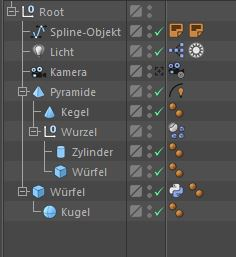
\includegraphics{Bilder/c4d_Szenengraph_Vgl.jpg}
	\caption{Der Cinema 4D Szenengraph. Verschiedenste Objekte als “Nodes”, daneben als Icons exemplarisch Tags verschiedener Tag-Datentypen am rechten Rand der Grafik.}
	\label{Cinema 4DSzenenGraph}
\end{figure}

Diese Objekte können wieder Kind-Objekte der gleichen Datentypen beinhalten. Diese Hierarchie zeigt die Abbildung \ref{Cinema 4DSzenenGraph}. Die in der Abbildung \ref{Cinema 4DSzenenGraph} am rechten Rand durch kleine Abbildungen neben den Nodes dargestellten Tags, beinhalten weitere Daten oder Einstellungen für das jeweils zugehörige Node. Diese können in einem anderen Fenster (Attribute Fenster/Panel) in Cinema 4d bearbeitet werden.

\subsubsection{Der Export einer Cinema 4D Szene in den Fusee Szenengraphen}
%TODO:  Wie kann der export stattfinden?
% Eventuell noch eine Grafik oder ein Ablaufdiagramm hierzu gestalten.
% Einen Algorithmus könnte ich eigentlich relativ simpel entwickeln.

\section{Stand der Implementierung}
Der folgende Abschnitt der Arbeit gibt nun einen Überblick über die bereits erfolgte Implementierung und zeigt welche Aufgaben sich mit dem zum Zeitpunkt der Arbeit bereits implementierten Teil der Software umsetzen lassen und welche Bereiche noch weiter entwickelt werden können und müssen.
\subsection{Bereits umgesetzte Module des Konzepts}
Während der Implementierungsphase wurde versucht mit Hilfe der Cinema 4D API und des Uniplug Projekts eine Softwarebibliothek zu implementieren welche Basisfunktionalität für die Verwendung von Cinema 4D als Authoring Tool bieten kann. 

Folgende Funktionalität wurde bereits umgesetzt:
\begin{itemize}
\item Ein \CSS Projekt kann in einem Binary Fusee Engine Projekt angelegt werden
\item Ein Projekt kann mit der Hilfe eines Plugins in Cinema 4D geöffnet werden
\item Eine neue \CSS Klasse kann mit der Bibliothek angelegt und in das Projekt integriert werden
\item Ein Tag kann im Cinema 4D Szenengraphen erzeugt und an ein Objekt der Szene geheftet werden
\item Verschiedene Module des Cinema 4D Plugins können untereinander über das Cinema 4D Message System Informationen austauschen
%TODO \item Eine Code Datei kann mit Hilfe eines Tags in Cinema 4D an ein Objekt angehängt werden. Hierzu wird im Speicher eine XML Datei angelegt und auf die Festplatte geschrieben, welche die Assoziation der beiden Objekte beschreibt.
\end{itemize}

Auf die genauere Umsetzung und einzelne interessante Aspekte der Implementierung wird in den nächsten Abschnitten weiter eingegangen.

\subsubsection{Implementierung: Generieren eines Fusee Projektes}
Um ein Projekt für die Fusee Engine zu generieren, wird die folgende Funktion \ref{CreateProjectMethod} des FuseeAT eingesetzt. 
\begin{lstlisting}[label=CreateProjectMethod, caption=Funktion zum Generieren eines neuen Projekts in der Binary Version der Fusee Engine.]
	public bool CreateProject(String slnName, String pName, String pPath);
\end{lstlisting}
Das Projekt kann durch die Angabe des Namens des Fusee Binary Solution Files, des vom Benutzer wählbaren Projektnamens und eines Pfades zur Solution erzeugt werden. Diese Funktion ist unabhängig von Cinema 4D implementiert. Alle Funktionen des FuseeAT sind nicht von einem bestimmten Modeling oder Level Editor abhängig und können somit wiederverwendet werden sollte das FuseeAT auf einen anderen Editor angepasst werden.

\subsubsection{Implementierung: Öffnen eines Fusee Projektes in Cinema 4D}
Ein bereits angelegtes Fusee Projekt kann durch den Plugin Code auch in Cinema 4D geöffnet werden. Die hierzu nötige Funktion \ref{OpenProjectMethod} ist die folgende:
\begin{lstlisting}[label=OpenProjectMethod, caption=Funktion zum öffnen eines neuen Projekts in der Binary Version der Fusee Engine.]
	public ToolState OpenProject(String pName, String pPath);
\end{lstlisting}
Das gewünschte Projekt wird, falls existent, direkt aus einer XML Datei deserialisiert. Diese XML Datei enthält alle wichtigen Informationen über das Projekt. Hierzu gehören verschiedene Dateinamen als auch verschiedene Pfade welche beim ersten Erstellen eines Projektes generiert oder durch den Benutzer über Dialoge und Abfragen eingegeben werden. Die im Codebeispiel \ref{OpenProjectStruct} dargestellten Attribute unterstützen das XML System beim serialisieren und deserialisieren der Objekte.

\begin{lstlisting}[label=OpenProjectStruct, caption=Teil des Structs zum Serialisieren des Fusee Projektes aus Cinem a 4D. Die Serialisierung speichert das Projekt auf der Festplatte als lesbare XML Datei.]
[XmlElement("PathToSolutionFolder")]
public String PathToSolutionFolder;

[XmlElement("PathToProjectFolder")]
public String PathToProjectFolder;
\end{lstlisting}


Das Projekt wird nach der Deserialisierung im Speicher gehalten. So kann die Applikation, in diesem Fall das C4DPlugin dauerhaft auf alle wichtigen Informationen für die Verwaltung des Projektes zur Laufzeit zugreifen.

\subsubsection{Implementierung: Erzeugen einer neuen \CSS Klasse und Einfügen in das Projekt}
Das Erzeugen einer neuen Klasse kann über die Funktion \ref{CreateClassMethod} erreicht werden. Die erzeugte Klasse wird vom FuseeAT in das \CSS Projekt eingefügt. Der Nutzer muss nur den Namen der neuen \CSS Klasse übergeben. Die Klasse wird nach einem im FuseeAT abgelegten TEmplate erzeugt und enthält bis auf die Standardstrukturen einer \CSS Klasse (Klassendefinition und Konstruktor) keine weiteren Bestandteile. Das Template kann aber einfach in FuseeAT um gewünschte Settings erweitert werden.
\begin{lstlisting}[label=CreateClassMethod, caption=Funktion zum Erstellen einer neuen Klasse im \CSS Projekt.]
	public bool CreateNewClass(String pName);
\end{lstlisting}

\subsubsection{Implementierung: Erstellen eines Tags und Anfügen von Code an ein Asset}
Durch die Cinema 4D API und das wrappen der dort vorhandenen Funktionen nach \CSS ist es möglich in der Cinema 4D Applikation an Objekte ein Tag anzuhängen. Ein Tag ist ein Objekt im Speicher welches in Referenz mit dem anhängenden Objekt steht und dieses um weitere Funktionalität oder Optionen erweitert. Es ist möglich dem Tag verschiedene Funktionen zuzuweisen. Leider muss die Funktionalität des Tags sehr stark an Cinema 4D gekuppelt werden da seine gesamte Implementierung über die C4D API erfolgt.
Um Informationen an einem Tag zu speichern, wird das gleiche XML Serialisierungs und Deserialisierungs System eingesetzt welches auch beim Laden und Speichern eines Engine Projektes verwendet wird.

\subsubsection{Das ToolState System des FuseeAT}
Das FuseeAT ToolState System ist ein Konzept welches bei der Implementierung des Frameworks umgesetzt wurde. Das System besteht auf einem einfachen State Machine Konzept und erlaubt es dem Entwickler zur Identifizierung von Schwierigkeiten einige Enum Variablen als Returnwerte der Funktionen einzusetzen. Durch die Verwendung des Enums \ref{ToolState} können Probleme während der Laufzeit im FuseeAT System aufgedeckt werden. Das Konzept sieht vor, als return Werte der FuseeAT Funktionen jeweils einen Status des ToolState Enums zurückzugeben. So kann der Entwickler eines Plugins oder Editors auf diese Funktionen eingehen und vermeidet es so mit einem korrumpierten Projekt weiter zu arbeiten.
\begin{lstlisting}[label=ToolState, caption=ToolState System unterstützt beim verbessern der Stabilität des FuseeAT.]
    public enum ToolState {
        OK = 0,
        ERROR = 1,
        WARNING = 2,
    }
\end{lstlisting}

\subsubsection{Der ProjectState in FuseeAT}
Durch die simple Implementierung des Enums ProjectState \ref{ProjectState} und dessen Verwendung während der Laufzeit des FuseeAT kann der Status des Projektes jederzeit überprüft werden. Ein Entwickler, welcher das FuseeAT erweitern oder verwenden möchte, kann jederzeit auf den Status des Projektes zugreifen und seine Funktionen mit absichern. Durch dieses recht einfache Konzept, können Probleme in den Solution und Projektdateien des FuseeAT erkannt werden. Es ist aber unabdingbar, dass fehleranfällige Operationen und Code diese Funktion auch einbinden und abfragen.
\begin{lstlisting}[caption=Code des ProjectState Enums. Wird in FuseeAT verwendet um die Integrität eines Projekts zu erhalten., label=ProjectState]
    public enum ProjectState
    {
        Clean = 0, // means open, too
        Dirty = 1,
        Corrupt = 2,
        Closed = 3
    }
\end{lstlisting}


%\subsection{Implementierung: Ablaufdiagramme}
%TODO: Hier noch etwas zu den Abläufen des Systems besonders des Plugins schreiben.

\subsection{Problematische Aspekte während der Implementierung}
Problematisch war, dass die Uniplug Softwarebibliothek zum Zeitpunkt der Implementierung nicht die nötigen Funktionen der Cinema 4D API unterstützte. Zudem wurde die Cinema 4D API Bibliothek und deren Integration in die Cinema 4D R16 Applikation während der Entwicklung durch ein Update seitens Maxon stark verändert und Uniplug musste daraufhin erneut auf die API angepasst werden. Um die Entwicklung des Plugins für die Verwendung der FuseeAT bibliothek zu beginnen, wurden verschiedenste  Funktionen der Cinema 4D API in das Uniplug Projekt integriert. Die Phase dieser Integration konnte aufgrund der Komplexität des Cinema 4D API nicht als abgeschlossen betrachtet werden. Während der Entwicklung des Plugins und des FuseeAT musste immer weitere Cinema 4D API Bestandteile nach \CSS gewrapped werden um die Funktionalität zwischen FuseeAT und dem Cinema 4D Plugin herzustellen. Da Uniplug ein essentielles Projekt für die Implementierung des Konzeptes darstellt, war es unerlässlich zuerst die fehlende Funktionalität in Uniplug zu ergänzen was einen großen Anteil an der Entwicklungszeit beanspruchte.

Die Komplexität der Cinema 4D \CPP API und dessen Transformation nach \CSS verzögerte die Entwicklung des Authoring Tool Frameworks und des Plugins deutlich, so dass während der Arbeit nicht alle geplanten Funktionen implementiert werden konnten. Hierzu zählt vor allem die GUI repräsentation der einzelnen Funktionen als auch das Build System.Weiterhin existieren aktuell nur schwer zu lösende Probleme welche durch die Verwendung von SWIG  in Verbindung mit der komplexen API von C4d auftraten. Die Funktionalität der User Interface Erweiterungen in Cinema 4D ist nur eingeschränkt vorhanden. Es ist aktuell nicht möglich, Cinema 4D GUI Fenster mit UI Elementen wie z.B. Buttons und Textfeldern zu erweitern. Es wurde versucht das System zu debuggen um den Grund für diese Problematik zu beheben. Allerdings konnte aufgrund des verschleierten Cinema 4D API Codes nur auf ein gewisses Level debugged werden. So ergibt sich beim Hinzufügen einer UI Komponentenen ein Fehler welcher nur bis zum Aufruf des Cinema 4D API Codes verfolgt werden konnte. Dort endet die Möglichkeit des Debuggings. Diese Komponente returned dann nur eine Boolean Variable mit der Belegung false. Aufgrund der zeitlichen beschränkung dieser Arbeit wurde dieses Modul ersteinmal hinten angestellt und die Entwicklung auf andere Teile des Konzepts konzentriert.

Weiterhin verkompliziert sich die Entwicklung durch das wrappen der \CPP Api nach \CSS stark. Einfache Funktionen der Cinema 4D API können meist nur kompliziert nach \CSS übersetzt werden. Hier zeigt sich ein Nachteil des Uniplug Projektes. Es ist zwar einfach, während der Entwicklung in \CSS gegebene Funktionen von Uniplug zu verwenden, allerdings ist die Erweiterung von Uniplug fast immer mit Problemen und großem Zeitaufwand verbunden. Somit erschwerte die immer wieder nötige Rückkehr nach Uniplug während der Implementierung das FuseeAT den effektiven Fortschritt massiv.

%\subsection{Ein Anwendungsgebiet für die Implementierung: XPresso Schaltungen - Visual Programming / Programmieren ohne das schreiben von Code}
% TODO: Hierzu gab es ein Paper auf welches ich gut verweisen könnte. Eventuell auch auf den Sony Editor welcher so eine Node basierte Programmierung bieten kann etc.
%Ein Ausblick auf die Zukunft. Eventuell hier den Artikel anführen welcher über Visuelle Programmierung berichtet hat.
% Eventuell ein verweis auf Uniplugs Ausgangsprojekt von damals. Die Programmierung mit XPressoNodes



%%%%%%
%	Hauptteil ENDE
%%%%%%


%%%%%%
%	Schluss START
%%%%%%
\chapter{Ergebnisse der Arbeit und Ausblick}
\section{Wie weit ist das Projekt fortgeschritten?}
Die Konzeption eines Authoring-Tools und die Untersuchung und Entwicklung eines Arbeitsprozesses für das Entwickeln von Authoring Tools in internen Teams wurde abgeschlossen. Der Arbeitsprozess beschreibt eine unbürokratische Möglichkeit zur Entwicklung von Tools und betrachtet hierbei sowohl Aspekte des Projektmanagements einer Tool Entwicklung als auch technische Aspekte. Der Prozess wurde grundsätzlich auf kleine interne Teams ausgerichtet und versucht das Projektmanagement mit so wenig Overhead\footnote{Zusätzlicher Aufwand durch Managementaufgaben welcher die Umsetzung des Projekts verzögert.} wie möglich umzusetzen. Weiterhin wurden zwei weitere Game Engines und deren Workflows und Ansätze untersucht. Die Szenengraphen der jeweiligen Engines wurden so weit es möglich war analysiert und gewonnene Erkenntnisse in ein Konzept für die Fusee Engine und das FuseeAT übersetzt. Das FuseeAT wurde während des Systemdesigns unabhängig einer speziellen Oberfläche entwickelt. Das Konzept für das FuseeAT wurde anschließend in der Implementierungsphase teilweise umgesetzt um ein Framework mit Schnittstellen nach Außen zu schaffen. Eine grundsätzliche Funktionalität ist gegeben und kann nun in verschiedene Editoren wie z.B. Cinema 4D integriert werden. Das Cinema 4D Plugin wurde in seinen Grundzügen erstellt und kann jederzeit erweitert werden. Das Uniplug Projekt umfasst noch nicht alle nötigen API Funktionen aber unterstützt aktuell die nötige Funktionalität um das Plugin zu testen.

\section{Integration des Systems in den weiteren Projektverlauf von Fusee}
Die im Abschnitt “Problematische Aspekte während der Implementierung” aufgeführten Probleme beeinflussten die Entwicklung des Cinema 4D Plugins stark negativ. Aus diesem Grund ist die Implementierung des FuseeAT nicht komplett abgeschlossen. Das Fusee Projekt an sich ist entsprechend seiner Natur als in der Lehre eingesetzte Simulations- und Entertainment Engine ein Projekt welches sich in ständiger Entwicklung befindet. Somit kann in Zukunft das FuseeAT für verschiedene Editoren und Tools genutzt werden um eine grafische Oberfläche für das Produzieren von Applikationen mit der Fusee Engine zu schaffen.  

%\subsection{Game Authoring Entwicklungsprozesse jetzt und in Zukunft}

\section{Fazit}
Aufgrund der gewonnenen Erkenntnisse lässt sich sagen, dass die Authoring Tool Entwicklung  auch in Zukunft ein wichtiger Bestandteil der Spiele und Software Entwicklung bleiben wird und seinen Einfluss auf das erfolgreiche Abschliessen von Projekten sicherlich noch weiter vergrößert. Verschiedenste angeführte Quellen belegen, dass dieser Bereich der Projekte immer weiter strukturiert und ausgebaut wird. Hierbei sei noch einmal auf Sonys Studio SnSystems\footnote{\url{http://snsystems.com/}} verwiesen welches sich rein um diese Aufgabe kümmert. Es ist aber auch für kleine Teams möglich während der Entwicklung Lücken im Tool Lineup des Unternehmens zu füllen und mit Hilfe von Frameworks und effizienter Planung schnell neue Tools zu erschaffen.
Um die Tool Entwicklung noch effizienter schneller zu gestalten wurde im Konzept zu FuseeAT besonders darauf geachtet, das FuseeAT Framework ungebunden von Editor Software zu gestalten. FuseeAT kann durch seinen Aufbau als modulares Framework schnell und unkompliziert erweitert werden. Die Schnittstelle zu FuseeAT steht als Interface bereit. Cinema 4D wiederum konnte aufgrund der gesetzten Ziele (Entwicklung des Frameworks in \CS, Anbindung an Cinema 4D mit dem Uniplug Projekt) nicht als effizientes Werkzeug für die Tool Entwicklung identifiziert werden. Die Idee, ein Authoring Tool so zu gestalten, dass jedes Mitglied des Teams seine gewohnte Arbeitsumgebung während der Entwicklung mit dem Tool nicht verlassen muss, scheiterte hier an der komplexen API und dem “Wrapping” der Cinema 4D API von \CPP nach \CSS. Das Konzept an sich scheint allerdings aufgrund der in der Untersuchung von Unity3d und der Unreal Engine 4 erkannten ähnlichen Konzepte einer 3DModelling Software und eines Game Engine Editors vielversprechend. Hier ergab sich ein größtenteils Deckungsgleiches Bild der Softwarearchitektur. Sicherlich kann die FuseeAT durch einen höheren Zeitaufwand und ein größeres Entwicklerteam in die Cinema 4D Software integriert werden.
Letztendlich wurden viele Grundsteine für die Entwicklung von und mit FuseeAT gelegt und ein kompletter Entwicklungsprozess für die Tool Entwicklung aufgezeigt. Eine Erweiterung der Implementierung findet in Zukunft sicherlich statt. Das Projekt wurde in die Fusee Engine integriert und kann als Open Source Software jederzeit eingesehen, angepasst und verändert werden.



%%%%%%
%	Schluss ENDE
%%%%%%


%%%%%%%%%%%%%%%%%%%%%%%%%%%%%%%%%%%%%%%%%%%%%%%%%%%%%%%%%%%%%%%%%%%%%%%%%%%%%%%%
% Inhalt ENDE
%%%%%%%%%%%%%%%%%%%%%%%%%%%%%%%%%%%%%%%%%%%%%%%%%%%%%%%%%%%%%%%%%%%%%%%%%%%%%%%%
\part*{Anhang}

%%%%%%%%%%%%%%%%%%%%%%%%%%%%%%%%%%%%%%%%%%%%%%%%%%%%%%%%%%%%%%%%%%%%%%%%%%%%%%%%
% Bilbiographie START
%%%%%%%%%%%%%%%%%%%%%%%%%%%%%%%%%%%%%%%%%%%%%%%%%%%%%%%%%%%%%%%%%%%%%%%%%%%%%%%%
%\nocite{*}
\addcontentsline{toc}{chapter}{Literaturverzeichnis}
%\cite{*}
\printbibliography
\newpage
%%%%%%%%%%%%%%%%%%%%%%%%%%%%%%%%%%%%%%%%%%%%%%%%%%%%%%%%%%%%%%%%%%%%%%%%%%%%%%%%
% Bilbiographie ENDE
%%%%%%%%%%%%%%%%%%%%%%%%%%%%%%%%%%%%%%%%%%%%%%%%%%%%%%%%%%%%%%%%%%%%%%%%%%%%%%%%

%%%%%%%%%%%%%%%%%%%%%%%%%%%%%%%%%%%%%%%%%%%%%%%%%%%%%%%%%%%%%%%%%%%%%%%%%%%%%%%%
% Source Code Verzeichnis START
%%%%%%%%%%%%%%%%%%%%%%%%%%%%%%%%%%%%%%%%%%%%%%%%%%%%%%%%%%%%%%%%%%%%%%%%%%%%%%%%
\lstlistoflistings

\newpage
\lstinputlisting[caption = {Beispiel zum Fusee Szenengraphen. Erstellt im Rahmen dieser Arbeit, während der Implementierung des Fusee Szenengraphen durch das Fusee Entwicklerteam und Herrn Prof. C. Müller.}, label=FuseeSzenenGraphExample]{Code/FuseeSzenenGraphExample.cs}

%%%%%%%%%%%%%%%%%%%%%%%%%%%%%%%%%%%%%%%%%%%%%%%%%%%%%%%%%%%%%%%%%%%%%%%%%%%%%%%%
% Source Code Verzeichnis ENDE
%%%%%%%%%%%%%%%%%%%%%%%%%%%%%%%%%%%%%%%%%%%%%%%%%%%%%%%%%%%%%%%%%%%%%%%%%%%%%%%%

%%%%%%%%%%%%%%%%%%%%%%%%%%%%%%%%%%%%%%%%%%%%%%%%%%%%%%%%%%%%%%%%%%%%%%%%%%%%%%%%
% Tabellen Verzeichnis START
%%%%%%%%%%%%%%%%%%%%%%%%%%%%%%%%%%%%%%%%%%%%%%%%%%%%%%%%%%%%%%%%%%%%%%%%%%%%%%%%
%\listoftables
%%%%%%%%%%%%%%%%%%%%%%%%%%%%%%%%%%%%%%%%%%%%%%%%%%%%%%%%%%%%%%%%%%%%%%%%%%%%%%%%
% Tabellen Verzeichnis ENDE
%%%%%%%%%%%%%%%%%%%%%%%%%%%%%%%%%%%%%%%%%%%%%%%%%%%%%%%%%%%%%%%%%%%%%%%%%%%%%%%%

%%%%%%%%%%%%%%%%%%%%%%%%%%%%%%%%%%%%%%%%%%%%%%%%%%%%%%%%%%%%%%%%%%%%%%%%%%%%%%%%
% Abbildungsverzeichnis START
%%%%%%%%%%%%%%%%%%%%%%%%%%%%%%%%%%%%%%%%%%%%%%%%%%%%%%%%%%%%%%%%%%%%%%%%%%%%%%%%
\listoffigures
%%%%%%%%%%%%%%%%%%%%%%%%%%%%%%%%%%%%%%%%%%%%%%%%%%%%%%%%%%%%%%%%%%%%%%%%%%%%%%%%
% Abbildungsverzeichnis ENDE
%%%%%%%%%%%%%%%%%%%%%%%%%%%%%%%%%%%%%%%%%%%%%%%%%%%%%%%%%%%%%%%%%%%%%%%%%%%%%%%%

%%%%%%%%%%%%%%%%%%%%%%%%%%%%%%%%%%%%%%%%%%%%%%%%%%%%%%%%%%%%%%%%%%%%%%%%%%%%%%%%
% UML START
%%%%%%%%%%%%%%%%%%%%%%%%%%%%%%%%%%%%%%%%%%%%%%%%%%%%%%%%%%%%%%%%%%%%%%%%%%%%%%%%
%\chapter*{UML Diagramme}
\addcontentsline{toc}{chapter}{System Design Diagramme}
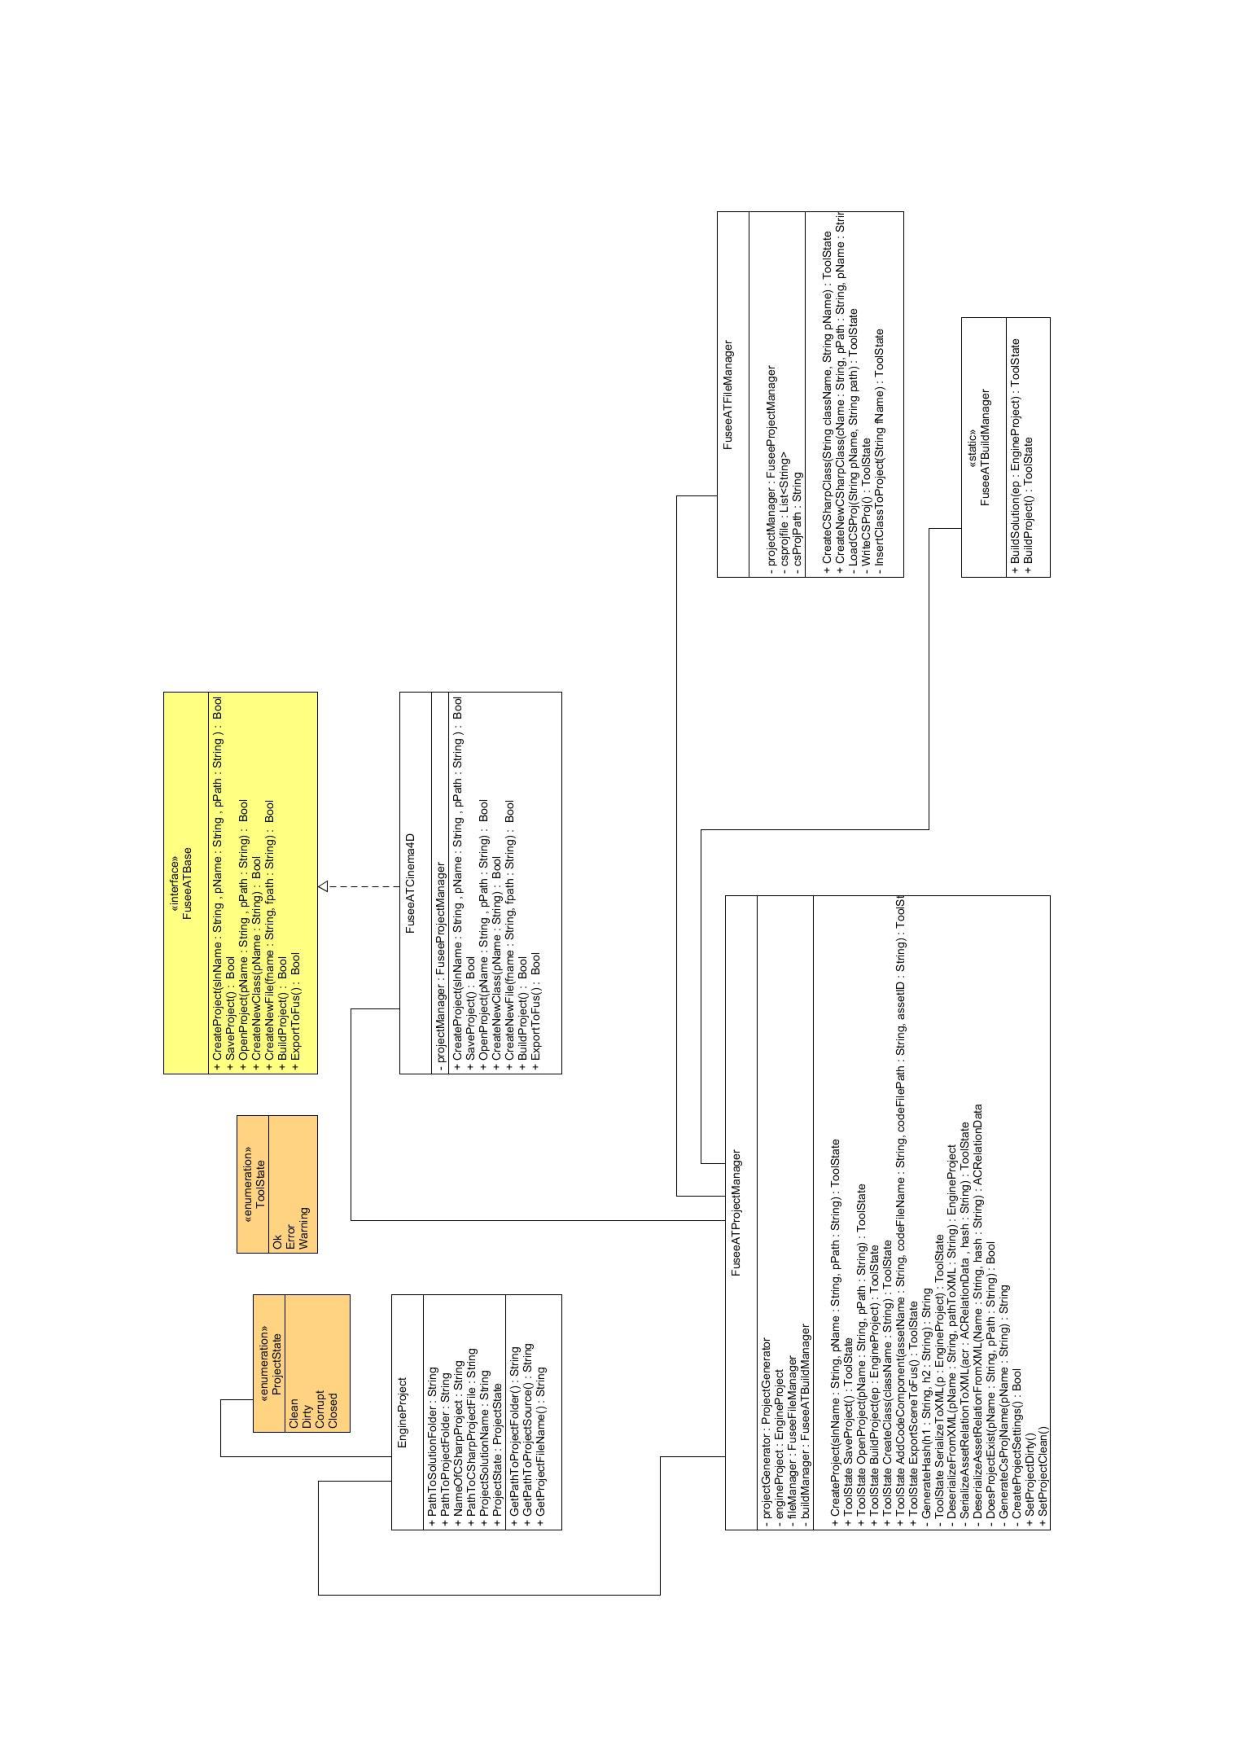
\includepdf[pages = 1-5]{Includes/UML_Sammlung.pdf}
%%%%%%%%%%%%%%%%%%%%%%%%%%%%%%%%%%%%%%%%%%%%%%%%%%%%%%%%%%%%%%%%%%%%%%%%%%%%%%%%
% UML ENDE
%%%%%%%%%%%%%%%%%%%%%%%%%%%%%%%%%%%%%%%%%%%%%%%%%%%%%%%%%%%%%%%%%%%%%%%%%%%%%%%%

%%%%%%%%%%%%%%%%%%%%%%%%%%%%%%%%%%%%%%%%%%%%%%%%%%%%%%%%%%%%%%%%%%%%%%%%%%%%%%%%
% Requirements START
%%%%%%%%%%%%%%%%%%%%%%%%%%%%%%%%%%%%%%%%%%%%%%%%%%%%%%%%%%%%%%%%%%%%%%%%%%%%%%%%
%\chapter*{Requirements Dokumente}
\addcontentsline{toc}{chapter}{Requirements Dokumente}
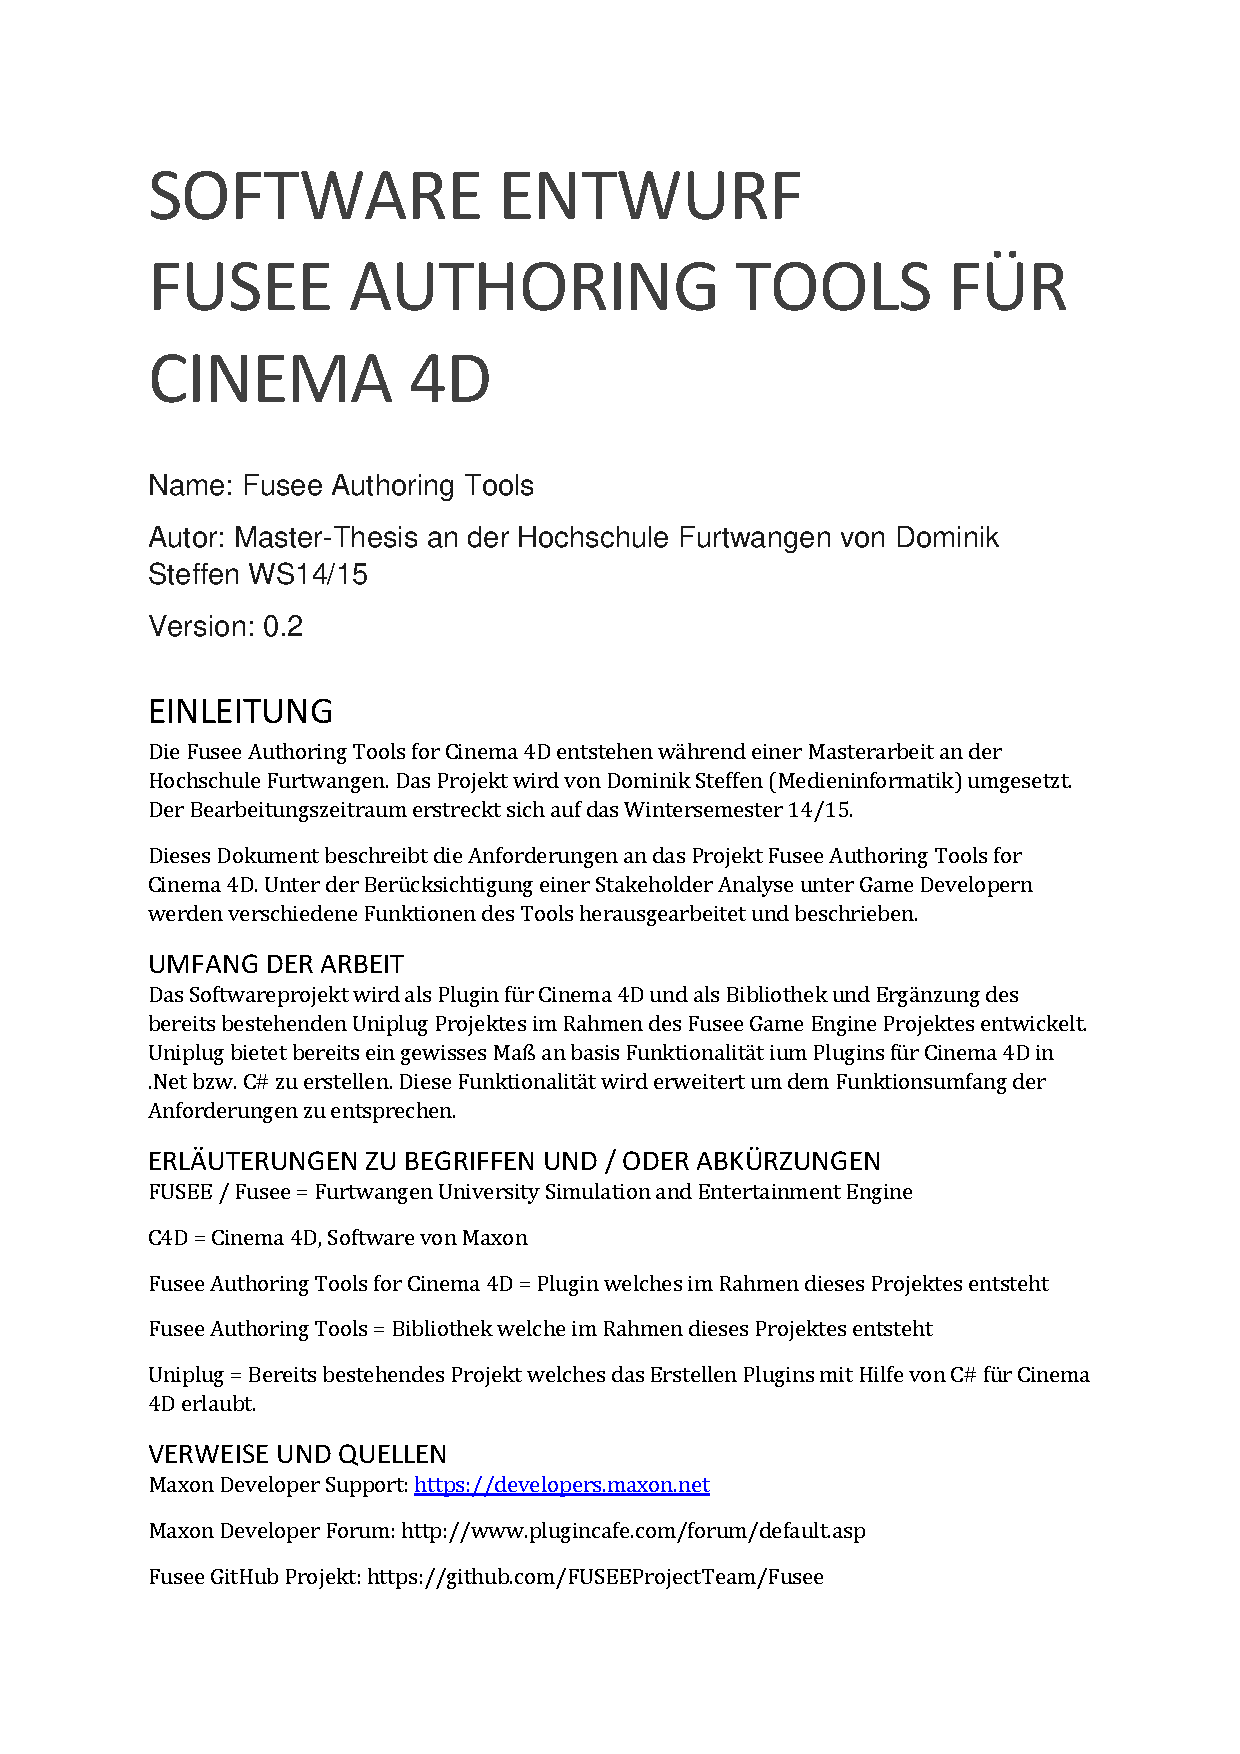
\includepdf[pages = 1-4]{Includes/SoftwareRequirementsSpecification.pdf}
%%%%%%%%%%%%%%%%%%%%%%%%%%%%%%%%%%%%%%%%%%%%%%%%%%%%%%%%%%%%%%%%%%%%%%%%%%%%%%%%
% Requirements ENDE
%%%%%%%%%%%%%%%%%%%%%%%%%%%%%%%%%%%%%%%%%%%%%%%%%%%%%%%%%%%%%%%%%%%%%%%%%%%%%%%%

\end{document}
